\documentclass[11pt,oneside]{book}
% Shared preamble for the Computer Science course notes.
% Each course has a main.tex that does % Shared preamble for the Computer Science course notes.
% Each course has a main.tex that does % Shared preamble for the Computer Science course notes.
% Each course has a main.tex that does \input{../common/preamble} and then
% \include's one file per chapter/lecture from its chapters/ directory.
%------------------------------------------------------------------------------
\usepackage[utf8]{inputenc}
\usepackage[T1]{fontenc}
\usepackage[english]{babel}
\usepackage{lmodern}
\usepackage[margin=1in]{geometry}
\usepackage{mathtools}
\usepackage{amsmath}
\usepackage{amssymb}
\usepackage{amsthm}
\usepackage{enumitem}
\usepackage{booktabs}
\usepackage{array}
\usepackage{graphicx}
\usepackage{float}
\usepackage{xcolor}
\usepackage{listings}
\usepackage{tikz}
\usepackage[most]{tcolorbox}
\usepackage[hidelinks]{hyperref}

\usetikzlibrary{arrows.meta,positioning,shapes,calc,trees,automata}

%------------------------------------------------------------------------------
% Math shortcuts (same names as the Math 239 notes)
\newcommand{\N}{\mathbb{N}}
\newcommand{\Z}{\mathbb{Z}}
\newcommand{\Q}{\mathbb{Q}}
\newcommand{\R}{\mathbb{R}}
\newcommand{\C}{\mathbb{C}}
\newcommand{\bigO}{\mathcal{O}}
\newcommand{\floor}[1]{\left\lfloor #1 \right\rfloor}
\newcommand{\ceil}[1]{\left\lceil #1 \right\rceil}
\newcommand{\abs}[1]{\left\lvert #1 \right\rvert}
\newcommand{\code}[1]{\texttt{#1}}

%------------------------------------------------------------------------------
% Theorem-like environments (numbered per chapter)
\theoremstyle{definition}
\newtheorem{definition}{Definition}[chapter]
\newtheorem{example}[definition]{Example}
\theoremstyle{plain}
\newtheorem{theorem}[definition]{Theorem}
\newtheorem{lemma}[definition]{Lemma}
\newtheorem{corollary}[definition]{Corollary}
\theoremstyle{remark}
\newtheorem*{remark}{Remark}

% Boxes: "important" for exam-relevant facts, "aside" for side comments.
\newtcolorbox{important}[1][]{colback=blue!4,colframe=blue!50!black,
  fonttitle=\bfseries,title={#1},boxrule=1pt}
\newtcolorbox{aside}{colback=gray!5,colframe=gray!60,boxrule=0.4pt}

%------------------------------------------------------------------------------
% Code listings
\definecolor{codebg}{gray}{0.96}
\definecolor{codecomment}{rgb}{0.25,0.5,0.35}
\definecolor{codekeyword}{rgb}{0.1,0.2,0.6}
\definecolor{codestring}{rgb}{0.6,0.1,0.1}
\lstset{
  basicstyle=\ttfamily\small,
  backgroundcolor=\color{codebg},
  commentstyle=\color{codecomment}\itshape,
  keywordstyle=\color{codekeyword}\bfseries,
  stringstyle=\color{codestring},
  columns=fullflexible,
  keepspaces=true,
  showstringspaces=false,
  breaklines=true,
  frame=single,
  rulecolor=\color{gray!40},
  tabsize=4,
  upquote=true,
  literate={~}{{\textasciitilde}}1
}

\lstdefinelanguage{Racket}{
  morekeywords={define,lambda,cond,else,if,let,let*,letrec,local,struct,
    define-struct,and,or,not,empty,cons,first,rest,list,check-expect,
    require,provide,begin,set!,when,unless,quote},
  sensitive=true,
  morecomment=[l]{;},
  morecomment=[s]{\#|}{|\#},
  morestring=[b]",
  alsoletter={-?!*>/+=<},
}

\lstdefinelanguage{MIPS}{
  morekeywords={add,addi,addu,sub,subu,mult,multu,div,divu,mfhi,mflo,lis,
    lw,sw,slt,sltu,beq,bne,jr,jalr,j,jal,and,or,xor,nor,sll,srl,lui,ori,word},
  sensitive=false,
  morecomment=[l]{;},
  morecomment=[l]{\#},
  alsoletter={.},
}

\lstdefinestyle{c}{language=C}
\lstdefinestyle{cpp}{language=C++}
\lstdefinestyle{racket}{language=Racket}
\lstdefinestyle{bash}{language=bash}
\lstdefinestyle{mips}{language=MIPS}
 and then
% \include's one file per chapter/lecture from its chapters/ directory.
%------------------------------------------------------------------------------
\usepackage[utf8]{inputenc}
\usepackage[T1]{fontenc}
\usepackage[english]{babel}
\usepackage{lmodern}
\usepackage[margin=1in]{geometry}
\usepackage{mathtools}
\usepackage{amsmath}
\usepackage{amssymb}
\usepackage{amsthm}
\usepackage{enumitem}
\usepackage{booktabs}
\usepackage{array}
\usepackage{graphicx}
\usepackage{float}
\usepackage{xcolor}
\usepackage{listings}
\usepackage{tikz}
\usepackage[most]{tcolorbox}
\usepackage[hidelinks]{hyperref}

\usetikzlibrary{arrows.meta,positioning,shapes,calc,trees,automata}

%------------------------------------------------------------------------------
% Math shortcuts (same names as the Math 239 notes)
\newcommand{\N}{\mathbb{N}}
\newcommand{\Z}{\mathbb{Z}}
\newcommand{\Q}{\mathbb{Q}}
\newcommand{\R}{\mathbb{R}}
\newcommand{\C}{\mathbb{C}}
\newcommand{\bigO}{\mathcal{O}}
\newcommand{\floor}[1]{\left\lfloor #1 \right\rfloor}
\newcommand{\ceil}[1]{\left\lceil #1 \right\rceil}
\newcommand{\abs}[1]{\left\lvert #1 \right\rvert}
\newcommand{\code}[1]{\texttt{#1}}

%------------------------------------------------------------------------------
% Theorem-like environments (numbered per chapter)
\theoremstyle{definition}
\newtheorem{definition}{Definition}[chapter]
\newtheorem{example}[definition]{Example}
\theoremstyle{plain}
\newtheorem{theorem}[definition]{Theorem}
\newtheorem{lemma}[definition]{Lemma}
\newtheorem{corollary}[definition]{Corollary}
\theoremstyle{remark}
\newtheorem*{remark}{Remark}

% Boxes: "important" for exam-relevant facts, "aside" for side comments.
\newtcolorbox{important}[1][]{colback=blue!4,colframe=blue!50!black,
  fonttitle=\bfseries,title={#1},boxrule=1pt}
\newtcolorbox{aside}{colback=gray!5,colframe=gray!60,boxrule=0.4pt}

%------------------------------------------------------------------------------
% Code listings
\definecolor{codebg}{gray}{0.96}
\definecolor{codecomment}{rgb}{0.25,0.5,0.35}
\definecolor{codekeyword}{rgb}{0.1,0.2,0.6}
\definecolor{codestring}{rgb}{0.6,0.1,0.1}
\lstset{
  basicstyle=\ttfamily\small,
  backgroundcolor=\color{codebg},
  commentstyle=\color{codecomment}\itshape,
  keywordstyle=\color{codekeyword}\bfseries,
  stringstyle=\color{codestring},
  columns=fullflexible,
  keepspaces=true,
  showstringspaces=false,
  breaklines=true,
  frame=single,
  rulecolor=\color{gray!40},
  tabsize=4,
  upquote=true,
  literate={~}{{\textasciitilde}}1
}

\lstdefinelanguage{Racket}{
  morekeywords={define,lambda,cond,else,if,let,let*,letrec,local,struct,
    define-struct,and,or,not,empty,cons,first,rest,list,check-expect,
    require,provide,begin,set!,when,unless,quote},
  sensitive=true,
  morecomment=[l]{;},
  morecomment=[s]{\#|}{|\#},
  morestring=[b]",
  alsoletter={-?!*>/+=<},
}

\lstdefinelanguage{MIPS}{
  morekeywords={add,addi,addu,sub,subu,mult,multu,div,divu,mfhi,mflo,lis,
    lw,sw,slt,sltu,beq,bne,jr,jalr,j,jal,and,or,xor,nor,sll,srl,lui,ori,word},
  sensitive=false,
  morecomment=[l]{;},
  morecomment=[l]{\#},
  alsoletter={.},
}

\lstdefinestyle{c}{language=C}
\lstdefinestyle{cpp}{language=C++}
\lstdefinestyle{racket}{language=Racket}
\lstdefinestyle{bash}{language=bash}
\lstdefinestyle{mips}{language=MIPS}
 and then
% \include's one file per chapter/lecture from its chapters/ directory.
%------------------------------------------------------------------------------
\usepackage[utf8]{inputenc}
\usepackage[T1]{fontenc}
\usepackage[english]{babel}
\usepackage{lmodern}
\usepackage[margin=1in]{geometry}
\usepackage{mathtools}
\usepackage{amsmath}
\usepackage{amssymb}
\usepackage{amsthm}
\usepackage{enumitem}
\usepackage{booktabs}
\usepackage{array}
\usepackage{graphicx}
\usepackage{float}
\usepackage{xcolor}
\usepackage{listings}
\usepackage{tikz}
\usepackage[most]{tcolorbox}
\usepackage[hidelinks]{hyperref}

\usetikzlibrary{arrows.meta,positioning,shapes,calc,trees,automata}

%------------------------------------------------------------------------------
% Math shortcuts (same names as the Math 239 notes)
\newcommand{\N}{\mathbb{N}}
\newcommand{\Z}{\mathbb{Z}}
\newcommand{\Q}{\mathbb{Q}}
\newcommand{\R}{\mathbb{R}}
\newcommand{\C}{\mathbb{C}}
\newcommand{\bigO}{\mathcal{O}}
\newcommand{\floor}[1]{\left\lfloor #1 \right\rfloor}
\newcommand{\ceil}[1]{\left\lceil #1 \right\rceil}
\newcommand{\abs}[1]{\left\lvert #1 \right\rvert}
\newcommand{\code}[1]{\texttt{#1}}

%------------------------------------------------------------------------------
% Theorem-like environments (numbered per chapter)
\theoremstyle{definition}
\newtheorem{definition}{Definition}[chapter]
\newtheorem{example}[definition]{Example}
\theoremstyle{plain}
\newtheorem{theorem}[definition]{Theorem}
\newtheorem{lemma}[definition]{Lemma}
\newtheorem{corollary}[definition]{Corollary}
\theoremstyle{remark}
\newtheorem*{remark}{Remark}

% Boxes: "important" for exam-relevant facts, "aside" for side comments.
\newtcolorbox{important}[1][]{colback=blue!4,colframe=blue!50!black,
  fonttitle=\bfseries,title={#1},boxrule=1pt}
\newtcolorbox{aside}{colback=gray!5,colframe=gray!60,boxrule=0.4pt}

%------------------------------------------------------------------------------
% Code listings
\definecolor{codebg}{gray}{0.96}
\definecolor{codecomment}{rgb}{0.25,0.5,0.35}
\definecolor{codekeyword}{rgb}{0.1,0.2,0.6}
\definecolor{codestring}{rgb}{0.6,0.1,0.1}
\lstset{
  basicstyle=\ttfamily\small,
  backgroundcolor=\color{codebg},
  commentstyle=\color{codecomment}\itshape,
  keywordstyle=\color{codekeyword}\bfseries,
  stringstyle=\color{codestring},
  columns=fullflexible,
  keepspaces=true,
  showstringspaces=false,
  breaklines=true,
  frame=single,
  rulecolor=\color{gray!40},
  tabsize=4,
  upquote=true,
  literate={~}{{\textasciitilde}}1
}

\lstdefinelanguage{Racket}{
  morekeywords={define,lambda,cond,else,if,let,let*,letrec,local,struct,
    define-struct,and,or,not,empty,cons,first,rest,list,check-expect,
    require,provide,begin,set!,when,unless,quote},
  sensitive=true,
  morecomment=[l]{;},
  morecomment=[s]{\#|}{|\#},
  morestring=[b]",
  alsoletter={-?!*>/+=<},
}

\lstdefinelanguage{MIPS}{
  morekeywords={add,addi,addu,sub,subu,mult,multu,div,divu,mfhi,mflo,lis,
    lw,sw,slt,sltu,beq,bne,jr,jalr,j,jal,and,or,xor,nor,sll,srl,lui,ori,word},
  sensitive=false,
  morecomment=[l]{;},
  morecomment=[l]{\#},
  alsoletter={.},
}

\lstdefinestyle{c}{language=C}
\lstdefinestyle{cpp}{language=C++}
\lstdefinestyle{racket}{language=Racket}
\lstdefinestyle{bash}{language=bash}
\lstdefinestyle{mips}{language=MIPS}

% Shorter, non-uppercase running heads so long chapter titles fit.
\makeatletter
\renewcommand{\chaptermark}[1]{\markright{\if@mainmatter\thechapter.\ \fi #1}}
\makeatother
\setlength{\emergencystretch}{3em}
\title{CS 246 --- Object-Oriented Software Development}
\author{Vishesh Gupta}
\date{University of Waterloo \\ Winter 2018, Nomair Naeem}
\begin{document}
\frontmatter
\maketitle
\tableofcontents
\mainmatter
\chapter{Course Outline}
\begin{center}
\textit{January 4, 2018}
\end{center}

\section{Course Information}

\begin{tabular}{@{}ll@{}}
\toprule
Instructor & Nomair Naeem \\
Office & DC 3111 \\
Email & \code{nanaeem@uwaterloo.ca} \\
Office hours & Thursdays, 9:30--11:00 am \\
\bottomrule
\end{tabular}

\subsection*{About the Instructor}
Nomair Naeem is a CS advisor and instructor. He has (literally) begged to change
what he teaches: he wants to teach compilers, but he teaches CS 246.

\section{Marking Scheme}

\begin{center}
\begin{tabular}{@{}lr@{}}
\toprule
Component & Weight \\
\midrule
Assignments & 40\% \\
Midterm (February 27) & 20\% \\
Final exam (2.5 hours) & 40\% \\
\bottomrule
\end{tabular}
\end{center}

\subsection*{Assignments}
\begin{center}
\begin{tabular}{@{}lr@{}}
\toprule
Assignment & Weight \\
\midrule
A0 & required (0\%) \\
A1 & 5\% \\
A2 & 7\% \\
A3 & 7\% \\
A4 & 9\% \\
A5 (final project) & 12\% \\
\bottomrule
\end{tabular}
\end{center}

\subsection*{Assignment Submission}
Assignments are submitted to \textbf{Marmoset}, which takes the most recent,
on-time best score. Each assignment has public (``release'') tests and private
tests that are only run after the deadline.

\begin{important}[Submission rule]
You lose a mark from the assignment for using more than three submissions on
release tests, so test locally first.
\end{important}

\section{Modules}
\begin{enumerate}
  \item \textbf{Linux shell} (about 2 weeks): files, commands, redirection,
        pipes, regular expressions, permissions, shell scripts.
  \item \textbf{C++} (about 10 weeks): C++ as a ``better C'', classes, the
        Big~5, encapsulation, inheritance, polymorphism, templates, the STL,
        exceptions.
  \item \textbf{Tools}: \code{g++}, \code{make}, \code{gdb}, \code{valgrind},
        version control with \code{git}.
  \item \textbf{Software engineering}: UML, design patterns, coupling and
        cohesion, exception safety.
\end{enumerate}

\section*{Summary}
Three-part assessment (assignments, midterm, final); the course moves from the
Linux shell into C++ and object-oriented design, finishing with design patterns
and software-engineering principles.

\chapter{Lecture 1: The Linux Shell and File System}
\begin{center}
\textit{January 4, 2018}
\end{center}

\section{Module 1: The Linux Shell}

\begin{definition}
A \textbf{shell} is an interface to the operating system. The OS talks to the
hardware; the shell lets the user talk to the OS. With a shell we
\begin{enumerate}
  \item manipulate files, and
  \item run programs.
\end{enumerate}
\end{definition}

\subsection{Types of Shells}

\paragraph{Graphical shell.} Windows, macOS and Linux all have one: point and
click, drag and drop. Intuitive to use.

The big disadvantage of a graphical shell is that it is not very powerful:
every feature has to be explicitly implemented by somebody. For example, suppose
a folder contains a lot of files with the extension \code{.c} and we want to
rename all of them to have extension \code{.cc}. Unless someone built a ``bulk
rename'' button, we are stuck doing it one file at a time.

\paragraph{Command-line shell.} We type commands at a \emph{prompt} (basically
a blinking cursor). The biggest disadvantage is the steep learning curve; the big
advantage is that it is very powerful. You do not need someone to have
``supported'' a feature: you combine small commands to build the feature
yourself.

DOS used to be the command-line shell on PCs, but it has gotten stale.

\subsection{History of the Linux Shell}
The Linux command-line shell is a descendant of the original Unix shell (1970s),
called simply \emph{the shell} and written by Stephen Bourne. It had a dozen or
two commands. Over time many shells appeared:
\begin{itemize}
  \item the Korn shell (\code{ksh}),
  \item the C shell (\code{csh}), which became the Turbo C shell (\code{tcsh}).
\end{itemize}
By then the original shell was called the \emph{Bourne shell} (\code{sh}), and
its successor became the \textbf{Bourne Again Shell} (\code{bash}), which is
what we use in CS 246.

To check that you are running bash:
\begin{lstlisting}[style=bash]
$ echo $0
-bash
\end{lstlisting}
(\code{\$0} is the name of the currently running program; the leading \code{-}
means it is a login shell.)

\section{The Linux File System}

The file system is similar to the one on Windows. In Linux, there are files
which can contain other files.

\begin{definition}
A \textbf{directory} is a file that can contain other files. Other than that,
Linux does not really distinguish between files and directories.
\end{definition}

The Linux file system is a \textbf{tree}. The root of the tree is a directory
called the \textbf{root directory}, written \code{/}.

\begin{center}
\begin{tikzpicture}[level distance=11mm,
  level 1/.style={sibling distance=30mm},
  level 2/.style={sibling distance=18mm},
  every node/.style={font=\ttfamily\small}]
\node {/}
  child {node {bin}}
  child {node {usr}
    child {node {share}
      child {node {dict}
        child {node {words}}}}
    child {node {bin}}}
  child {node {u}
    child {node {nanaeem}}};
\end{tikzpicture}
\end{center}

\begin{definition}
A \textbf{path} specifies the location of a file in the file system. An
\textbf{absolute path} begins at the root directory, e.g.\
\code{/usr/share/dict/words}. A \textbf{relative path} starts at the current
directory.
\end{definition}

If \code{pwd} is \code{/Users/nanaeem}, then the absolute path
\code{/Users/nanaeem/cs246/a1} names the same directory as the relative path
\code{cs246/a1}.

\begin{aside}
Special directory names:
\begin{itemize}
  \item \code{.} is the current directory,
  \item \code{..} is the parent directory, \code{../..} the grandparent,
  \item \code{\textasciitilde} is your home directory, and
        \code{\textasciitilde userid} is \code{userid}'s home directory.
\end{itemize}
\end{aside}

\section{Basic Commands}

\begin{center}
\begin{tabular}{@{}lp{0.62\textwidth}@{}}
\toprule
Command & Meaning \\
\midrule
\code{clear} & clear the screen \\
\code{ls} & list the (non-hidden) files in the current directory \\
\code{ls -a} & list all files, including hidden ones (names starting with \code{.}) \\
\code{ls -l} & long listing (permissions, owner, size, date) \\
\code{pwd} & print the present working directory \\
\code{cd <path>} & change directory to \code{<path>} \\
\code{cd} & with no argument: go to your home directory \\
\code{cd -} & go back to the previous directory \\
\bottomrule
\end{tabular}
\end{center}

The \code{-a} in \code{ls -a} is called an \emph{option} (or \emph{flag}); it
modifies the behaviour of the command. Options can usually be combined, e.g.\
\code{ls -la}.

\begin{lstlisting}[style=bash]
$ cd /Users/nanaeem/cs246/a1    # absolute path
$ cd ..                          # now in /Users/nanaeem/cs246
$ cd a1                          # relative path, back in a1
$ pwd
/Users/nanaeem/cs246/a1
\end{lstlisting}

\section*{Summary}
\begin{itemize}
  \item A shell is an interface to the OS; command-line shells trade a learning
        curve for power. We use \code{bash}.
  \item The file system is a tree rooted at \code{/}; directories are files that
        contain files.
  \item Absolute paths start at \code{/}; relative paths start at the current
        directory, with \code{.}, \code{..}, \code{\textasciitilde} as shortcuts.
  \item First commands: \code{clear}, \code{ls}, \code{pwd}, \code{cd}.
\end{itemize}

\chapter{Tutorial 1: Getting Set Up}
\begin{center}
\textit{January 3, 2018}
\end{center}

Welcome to tutorial 1! (This surprisingly happened even before the first day of
classes.)

\section{Course Infrastructure}
CS 246 course content is distributed through \code{git}, so we will need some
\code{git} commands; they are explained as we go through the course.

A Linux environment is preferred (and recommended) for all work. All course
material is available on the Linux student server, and assignments are tested
there, so code should always be checked on the server before submitting.

\section{Logging In to the Student Server}
\begin{lstlisting}[style=bash]
ssh username@linux.student.cs.uwaterloo.ca
# then enter the password for this account
\end{lstlisting}
If you do not have any clue what your \code{linux.student.cs} password was
from CS 136, it can be reset through the CS Computing Facility account web page.

This method works directly on:
\begin{enumerate}
  \item Linux,
  \item macOS,
  \item Bash on Ubuntu on Windows (Windows Subsystem for Linux; Windows 10
        Creators Update or later). Setup instructions:
        \url{https://docs.microsoft.com/en-us/windows/wsl/about}.
\end{enumerate}
Otherwise, download the \textbf{PuTTY} client (a free \code{.exe}) or
\textbf{SuperPuTTY}.

\subsection*{Copying files}
Files can be copied to and from the server with \code{scp}:
\begin{lstlisting}[style=bash]
scp a1q1.cc username@linux.student.cs.uwaterloo.ca:~/cs246/a1/
scp username@linux.student.cs.uwaterloo.ca:~/cs246/a1/out.txt .
\end{lstlisting}

\section{Course Directory and A0}
The course account has a directory (\code{/u/cs246/}) that holds the current
term's material; older terms' material is kept in older directories. A0 has been
posted (Piazza has hints about where A0 lives each term).

\begin{important}[Advice]
Start the assignments early.
\end{important}

\section*{Summary}
Use the Linux student server (via \code{ssh}/PuTTY), get course material with
\code{git}, and complete A0 (which is required) early.

\chapter{Tutorial 2: Shell Commands, Streams, grep and Vim}
\begin{center}
\textit{January 10, 2018}
\end{center}

\section{List of Commands}

\begin{center}
\begin{tabular}{@{}lp{0.65\textwidth}@{}}
\toprule
Command & What it does \\
\midrule
\code{cd} & change directory; with no argument goes home; \code{cd -} goes back
            to the previous directory \\
\code{clear} & clear the screen \\
\code{ls} & list files, e.g.\ \code{ls ..}, \code{ls -l}, \code{ls -a} \\
\code{touch} & create an empty file (or update a file's timestamp) \\
\code{pwd} & display the present working directory \\
\code{cat} & print the contents of a file \\
\code{head} & print the first 10 lines (\code{head -n 5} for the first 5) \\
\code{tail} & print the last 10 lines \\
\code{sort} & sort lines in lexicographical order \\
\code{uniq} & remove \emph{adjacent} duplicate lines (so usually used after \code{sort}) \\
\code{shuf} & output a random permutation of the input lines \\
\code{tac} & like \code{cat} but prints the lines in reverse order \\
\code{wc} & count lines, words and characters \\
\bottomrule
\end{tabular}
\end{center}

\section{Input and Output Streams}
Think of a program as a black box with one input stream and two output streams:
\begin{itemize}
  \item \textbf{stdin}: by default the keyboard.
  \item \textbf{stdout}: by default the screen. stdout is \emph{buffered}: output
        is collected and written in blocks, since writing character by character
        is expensive.
  \item \textbf{stderr}: by default also the screen. stderr is \emph{not}
        buffered, so error messages appear immediately. Example: the nuclear
        reactor is about to explode --- we want to see that message \emph{now},
        not when the buffer fills up.
\end{itemize}
We will solidify these concepts when we do I/O in C++.

\begin{lstlisting}[style=bash]
g++ printer.cc -o print
./print > out.txt 2> err.txt   # stdout to out.txt, stderr to err.txt
./print &> all.txt             # all streams to all.txt
./print > all.txt 2>&1         # same: send stderr where stdout is going
\end{lstlisting}

\begin{important}[Stream numbers]
stdin is 0, stdout is 1, stderr is 2. \code{2>\&1} redirects stderr to the same
place as stdout; \code{\&>} redirects both. Order matters: \code{2>\&1} must come
\emph{after} \code{> file}.
\end{important}

\paragraph{Pipes.} \code{cmd1 | cmd2} connects stdout of \code{cmd1} to stdin of
\code{cmd2}.

\paragraph{Embedded commands.} \code{\$(cmd)} is replaced by the output of
\code{cmd}, e.g.\ \code{egrep "\$(cat pattern)" words.txt}.

\section{grep and Regular Expressions}
\code{grep} (and \code{egrep}, which uses extended regular expressions) prints
the lines of its input that match a pattern:
\begin{lstlisting}[style=bash]
egrep "int" wordcollection.txt
\end{lstlisting}

\begin{center}
\begin{tabular}{@{}cl@{}}
\toprule
Symbol & Meaning \\
\midrule
\code{\^{}} & match the beginning of the line \\
\code{\$} & match the end of the line \\
\code{.} & match any single character \\
\code{?} & the preceding item 0 or 1 times \\
\code{*} & the preceding item 0 or more times \\
\code{+} & the preceding item 1 or more times \\
\code{[ ]} & any one of the characters inside \\
\bottomrule
\end{tabular}
\end{center}

\section{Vim Commands}
\begin{center}
\begin{tabular}{@{}ll@{}}
\toprule
Keys & Effect \\
\midrule
\code{i} & enter insert mode (\code{Esc} returns to normal mode) \\
\code{Esc :w} & write (save) \\
\code{Esc :wq} & write and quit \\
\code{Esc :x} & save (only if there are changes) and quit \\
\code{Esc :xa} & do \code{:x} on all open buffers/tabs \\
\code{Esc :q!} & quit without saving \\
\code{u} & undo \\
\code{Ctrl-r} & redo \\
\code{dd}, \code{yy}, \code{p} & delete line, copy (yank) line, paste \\
\code{/text} & search forward for \code{text} \\
\bottomrule
\end{tabular}
\end{center}

\section*{Summary}
Know the basic file/text commands, the three standard streams and how to
redirect them (including \code{2>\&1}), pipes and \code{\$(...)}, basic regex
for \code{egrep}, and enough Vim to edit, save and quit.

\chapter{Lecture 2: Redirection, Globbing, Pipes and egrep}
\begin{center}
\textit{January 9, 2018}
\end{center}

\section{cat and Keyboard Signals}
\code{cat} stands for \emph{concatenate}; with file arguments it displays the
contents of the files one after another. With no arguments it echoes stdin to
stdout.

\begin{itemize}
  \item \textbf{Ctrl+C} --- kill the running program.
  \item \textbf{Ctrl+D} --- send the end-of-file (EOF) signal.
\end{itemize}

\section{Input and Output Redirection}

\begin{definition}
\textbf{Output redirection} sends the output produced by a program to a file:
\code{command arg1 arg2 ... > filename}.

\textbf{Input redirection} sends the contents of a file to a program as its
input: \code{command arg1 arg2 ... < filename}.
\end{definition}

\subsection*{\code{cat sample.txt} vs.\ \code{cat < sample.txt}}
The output is identical, but the mechanism is different:
\begin{itemize}
  \item \code{cat sample.txt}: \code{cat} is given a filename, \emph{cat} opens
        the file and displays its contents.
  \item \code{cat < sample.txt}: the \emph{shell} opens the file and sends its
        contents to \code{cat}'s stdin; \code{cat} never sees a filename.
\end{itemize}
\begin{center}
\begin{tikzpicture}[>=Stealth,font=\small,
  prog/.style={draw,fill=gray!15,minimum width=1.6cm,minimum height=0.9cm},
  file/.style={draw,fill=yellow!10,minimum height=0.7cm}]
  \node[prog] (c1) at (0,0) {\code{cat}};
  \node[file] (f1) at (-4.2,0) {\code{sample.txt}};
  \draw[->] (c1.west) -- node[above,font=\scriptsize]{opens (argument)} (f1.east);
  \node[font=\scriptsize,anchor=west] at (1.2,0) {\code{cat sample.txt}};
  \node[prog] (c2) at (0,-1.6) {\code{cat}};
  \node[file] (f2) at (-4.2,-1.6) {\code{sample.txt}};
  \node[draw,dashed,rounded corners,font=\scriptsize] (sh) at (-4.2,-2.6) {shell opens it};
  \draw[->] (f2.east) -- node[above,font=\scriptsize]{stdin} (c2.west);
  \draw[dashed] (sh) -- (f2);
  \node[font=\scriptsize,anchor=west] at (1.2,-1.6) {\code{cat < sample.txt}};
\end{tikzpicture}
\end{center}
The difference is visible with \code{wc}:
\begin{lstlisting}[style=bash]
$ wc sample.txt
 10  52 300 sample.txt
$ wc < sample.txt
 10  52 300
\end{lstlisting}

Input and output redirection can be combined (each used once):
\begin{lstlisting}[style=bash]
cmd arg1 arg2 ... < inputfile > outputfile
cat -n < in.txt > out.txt    # like cp, but numbers the lines
\end{lstlisting}

\section{Behind the Scenes: Three Streams}
Every Linux process (\code{ls}, \code{cat}, a C/C++ program, \dots) has three
streams associated with it.

\begin{center}
\begin{tabular}{@{}p{0.29\textwidth}p{0.29\textwidth}p{0.29\textwidth}@{}}
\toprule
stdin (standard input) & stdout (standard output) & stderr (standard error) \\
\midrule
Default: keyboard & Default: screen & Default: screen \\
Change with \code{<} & Change with \code{>} & Change with \code{2>} \\
 & Buffered & Not buffered \\
\bottomrule
\end{tabular}
\end{center}

\begin{aside}
\textbf{Buffering:} writing in blocks is faster than writing one character at a
time (you will see why in CS 350). stderr is unbuffered so error messages show up
immediately.
\end{aside}

\begin{lstlisting}[style=bash]
cmd >> out.txt               # append to the end of out.txt
cmd < in 1> out 2>&1         # stdout to out, stderr to the same place as stdout
\end{lstlisting}
\code{\&1} means ``wherever stream 1 (stdout) is currently going''.

\section{Wildcards and Globbing}
\begin{lstlisting}[style=bash]
ls *.txt
\end{lstlisting}
\code{*.txt} is a \textbf{globbing pattern}: \code{*} matches any sequence of
characters, so this lists all files whose names end with \code{.txt}.

The \emph{shell} intercepts the pattern:
\begin{enumerate}
  \item it finds the files that match the pattern, and
  \item replaces the pattern by those file names.
\end{enumerate}
So \code{ls} actually receives \code{ls sample.txt sample2.txt}. Because the
shell does the work, globbing works with any command:
\begin{center}
\begin{tikzpicture}[>=Stealth,font=\small,node distance=0.8cm]
  \node[draw,fill=yellow!10] (t) {\code{ls *.txt}};
  \node[draw,rounded corners,fill=blue!6,right=of t,align=center] (s) {shell\\ \scriptsize expands the glob};
  \node[draw,fill=yellow!10,right=of s] (t2) {\code{ls sample.txt sample2.txt}};
  \node[draw,fill=gray!15,right=of t2] (l) {\code{ls}};
  \draw[->] (t) -- (s); \draw[->] (s) -- (t2); \draw[->] (t2) -- (l);
\end{tikzpicture}
\end{center}
\begin{lstlisting}[style=bash]
cat *.txt
echo *.txt      # a cheap way to see what a pattern expands to
rm *.txt
rm -rf *        # careful!!
\end{lstlisting}
Other glob characters: \code{?} matches exactly one character, and \code{[abc]}
matches one of the listed characters.

\begin{important}[Quoting]
Single quotes and double quotes suppress globbing: \code{echo "*.txt"} prints
\code{*.txt}.
\end{important}

\section{Pipes}
We can send the output (stdout) of one program to the input (stdin) of another
with a \textbf{pipe}: \code{cmd1 | cmd2}.

\begin{example}
How many words occur in the first 20 lines of \code{sample.txt}?
\begin{lstlisting}[style=bash]
head -20 sample.txt | wc -w
\end{lstlisting}
\end{example}

\begin{example}
Files \code{words*.txt} contain lists of words, one per line. Print a
duplicate-free list of all the words in all the files.
\begin{lstlisting}[style=bash]
cat words*.txt | sort | uniq
\end{lstlisting}
\begin{center}
\begin{tikzpicture}[>=Stealth,font=\small,node distance=1.4cm,
  prog/.style={draw,fill=gray!15,minimum width=1.4cm,minimum height=0.8cm}]
  \node[prog] (a) {\code{cat}};
  \node[prog,right=of a] (b) {\code{sort}};
  \node[prog,right=of b] (c) {\code{uniq}};
  \node[right=of c] (d) {screen};
  \node[draw,fill=yellow!10,left=0.9cm of a,align=center,font=\scriptsize] (f) {\code{words1.txt}\\ \code{words2.txt}};
  \draw[->] (f) -- (a);
  \draw[->] (a) -- node[above,font=\scriptsize]{stdout} node[below,font=\scriptsize]{stdin} (b);
  \draw[->] (b) -- node[above,font=\scriptsize]{stdout} node[below,font=\scriptsize]{stdin} (c);
  \draw[->] (c) -- node[above,font=\scriptsize]{stdout} (d);
\end{tikzpicture}
\end{center}
\code{uniq} only removes \emph{adjacent} duplicates, which is why we
\code{sort} first.
\end{example}

\section{Embedded Commands}
Use \code{\$(cmd)} to embed the output of a command inside another command:
\begin{lstlisting}[style=bash]
echo "Today is $(date) and I am $(whoami)"
\end{lstlisting}
\begin{itemize}
  \item Double quotes allow embedded commands (and variables) but suppress
        globbing; they also keep the result as a \emph{single} argument.
  \item Single quotes suppress embedded commands as well:
        \code{echo 'Today is \$(date)'} prints the text literally.
  \item Without quotes, each whitespace-separated word is a separate argument.
\end{itemize}

\section{egrep}
\code{egrep pattern file(s)} prints the lines that contain a substring matching
the given pattern (a regular expression).
\begin{lstlisting}[style=bash]
egrep cs246 index.shtml | wc -l           # number of lines mentioning cs246
egrep "cs246|CS246" index.shtml | wc -l   # either spelling
\end{lstlisting}
\code{|} in a regular expression means ``or''. Use double quotes around patterns
containing characters that are special to the shell (\code{|}, \code{*},
\code{?}, \dots), otherwise the shell interprets them first.

\section*{Summary}
\begin{itemize}
  \item \code{>}, \code{>>}, \code{<}, \code{2>}, \code{2>\&1} redirect streams;
        the shell does the redirection, not the program.
  \item stdout is buffered, stderr is not.
  \item Globbing (\code{*}, \code{?}, \code{[...]}) is expanded by the shell;
        quotes suppress it.
  \item Pipes chain programs; \code{\$(...)} embeds a command's output.
  \item \code{egrep} searches for lines matching a regular expression.
\end{itemize}

\chapter{Lecture 3: Regular Expressions, Permissions, Variables and Scripts}
\begin{center}
\textit{January 11, 2018}
\end{center}

\section{Regular Expressions (continued)}
Last time: \code{egrep pattern file(s)}. For example
\begin{lstlisting}[style=bash]
egrep "(cs|CS)246" index.html
\end{lstlisting}
This is \emph{not} the same as \code{"(c|C)(s|S)246"} (which also matches
\code{cS246} and \code{Cs246}); that one can also be written
\code{"[cC][sS]246"}.

\begin{center}
\begin{tabular}{@{}lp{0.68\textwidth}@{}}
\toprule
Pattern & Matches \\
\midrule
\code{[abc]} & one character from the set, i.e.\ \code{(a|b|c)} \\
\code{[\^{}abc]} & one character \emph{not} from the set \\
\code{[a-z]} & one character in the range \\
\code{?} & 0 or 1 occurrences of the preceding expression \\
\code{*} & 0 or more occurrences of the preceding expression \\
\code{+} & 1 or more occurrences of the preceding expression \\
\code{.} & any one character \\
\code{.*} & any number of any characters \\
\code{\textbackslash.} & a literal \code{.} (backslash escapes a special symbol) \\
\code{\^{}} & forces the match to start at the beginning of the line \\
\code{\$} & forces the match to end at the end of the line \\
\bottomrule
\end{tabular}
\end{center}

Examples:
\begin{itemize}
  \item \code{"cs ?246"} matches \code{cs246} and \code{cs 246}.
  \item \code{"(cs)?246"} matches \code{cs246} or just \code{246}.
  \item \code{"\^{}cs246"}: lines starting with \code{cs246};
        \code{"\^{}cs246\$"}: lines containing exactly \code{cs246}.
\end{itemize}

\begin{example}
Print all words in \code{/usr/share/dict/words} that start with an \code{e} and
have length 5.
\begin{lstlisting}[style=bash]
egrep "^e....$" /usr/share/dict/words
\end{lstlisting}
\end{example}

\begin{example}
Lines of even length:
\begin{lstlisting}[style=bash]
egrep "^(..)*$" filename
\end{lstlisting}
\end{example}

\begin{important}[Anchors]
When a pattern must \emph{count} characters (exact length, exactly one
occurrence, \dots), anchor it with \code{\^{}} and \code{\$}. Otherwise
\code{egrep} happily matches a substring of the line.
\end{important}

\begin{example}
List the file names in the current directory that contain exactly one \code{a}.
\begin{lstlisting}[style=bash]
ls -a | egrep "^[^a]*a[^a]*$"
\end{lstlisting}
\end{example}

\section{File Permissions}
\code{ls -l} gives a long listing:
\begin{lstlisting}[style=bash]
-rwxr-xr--  1 nanaeem  staff  2048 Jan 11 10:00 script.sh
\end{lstlisting}
The columns are: type and permissions, number of links, owner, group, size,
last-modified date, and file name. The first character is \code{-} for an
ordinary file and \code{d} for a directory. The next nine characters are three
groups of three:

\begin{center}
\begin{tabular}{@{}ccc@{}}
\toprule
\code{rwx} & \code{r-x} & \code{r--} \\
user (owner) & group & other \\
\midrule
the file's owner & users in the file's group & everyone else \\
\bottomrule
\end{tabular}
\end{center}

\begin{center}
\begin{tabular}{@{}clp{0.42\textwidth}@{}}
\toprule
Bit & On an ordinary file & On a directory \\
\midrule
\code{r} & read the file & list the directory's contents (e.g.\ globbing) \\
\code{w} & modify the file & add/remove files in the directory \\
\code{x} & run the file as a program & enter the directory (\code{cd}) \\
\bottomrule
\end{tabular}
\end{center}

Only the owner can change a file's permissions, using \code{chmod mode file(s)}.
A mode consists of
\begin{enumerate}
  \item an ownership class: \code{u}ser, \code{g}roup, \code{o}ther, \code{a}ll;
  \item an operator: \code{+} (add), \code{-} (remove), \code{=} (set exactly);
  \item permissions: \code{r}, \code{w}, \code{x}.
\end{enumerate}
\begin{lstlisting}[style=bash]
chmod a+r final.pdf     # give everyone read permission
chmod g-rw final.pdf    # remove read and write from the group
chmod o=rx final.pdf    # set others to exactly read/execute
chmod u+x myscript      # make a script executable by me
\end{lstlisting}

\section{Shell Variables}
\begin{lstlisting}[style=bash]
x=1          # no spaces around = !  variables store strings
echo $x
echo ${x}    # recommended
\end{lstlisting}
When you \emph{write} a variable, no \code{\$}; when you \emph{read} it, use
\code{\$}. It is good practice to use curly braces around variable names:
\code{\$\{x\}abc} is unambiguous, \code{\$xabc} refers to a variable named
\code{xabc}.

\begin{itemize}
  \item Double quotes allow variable expansion; single quotes suppress it:
        \code{echo '\$\{x\}'} prints \code{\$\{x\}}.
  \item Variables last for the current session only. To set something
        permanently, put it in \code{\textasciitilde/.bash\_profile} (or
        \code{.bashrc}).
\end{itemize}

\subsection*{PATH}
\code{echo \$\{PATH\}} prints a list of directories separated by colons. When you
type a command, the shell searches these directories (in order) for a program
with that name.
\begin{lstlisting}[style=bash]
PATH=mypath:${PATH}    # search mypath first
PATH=${PATH}:mypath    # search mypath last
\end{lstlisting}

\section{Shell Scripts}
\begin{definition}
A \textbf{shell script} is a text file containing a sequence of shell commands
that can be executed as a program.
\end{definition}
\begin{itemize}
  \item The first line should be \code{\#!/bin/bash}, the \emph{shebang} (``hash
        bang'') line. It tells the OS to run the script with bash.
  \item Give the script executable permission: \code{chmod u+x script}.
  \item Run it with \code{./script} (the current directory is usually not in
        \code{PATH}).
\end{itemize}

\begin{lstlisting}[style=bash]
#!/bin/bash
date
whoami
pwd
\end{lstlisting}

\subsection{Arguments to a Script}
\begin{lstlisting}[style=bash]
./script arg1 arg2 ...
#  $0     $1   $2
\end{lstlisting}
\code{\$0} is the script's name, \code{\$1}, \code{\$2}, \dots{} are its arguments,
and \code{\$\#} is the number of arguments.

\begin{example}
Is a given word a valid word in the dictionary?
\begin{lstlisting}[style=bash]
#!/bin/bash
egrep "^$1$" /usr/share/dict/words
\end{lstlisting}
\end{example}

\subsection{Status Codes}
Every Linux command sets a \textbf{status code}, stored in \code{\$?}:
\code{0} means success, non-zero means failure. For \code{egrep}, success means
``found a match''.

\begin{aside}
To throw away output we don't care about, send it to \code{/dev/null}, a special
file that discards everything written to it.
\end{aside}

\subsection{Evaluating Conditions}
Conditions are evaluated with the \code{test} program, which can also be written
as \code{[ ... ]}. The spaces inside the brackets are mandatory, because
\code{[} is literally the name of a program and the rest are its arguments.

\begin{example}
A good password is a word that is \emph{not} in the dictionary. Is a given word a
good password?
\begin{lstlisting}[style=bash]
#!/bin/bash
# The answer is the script's own status code.
egrep "^$1$" /usr/share/dict/words > /dev/null
[ $? -ne 0 ]
\end{lstlisting}
The status of a script is the status of its last command, so the script
succeeds exactly when \code{egrep} failed to find the word.
\end{example}

\code{\#} starts a comment. \code{[ -e basic ]} checks whether a file named
\code{basic} exists.

\section*{Summary}
\begin{itemize}
  \item Regex: \code{[...]}, \code{[\^{}...]}, \code{?}, \code{*}, \code{+},
        \code{.}, \code{|}, grouping, and the anchors \code{\^{}} and \code{\$}.
  \item \code{ls -l} shows \code{rwx} permissions for user/group/other;
        \code{chmod} changes them.
  \item Variables: \code{x=1}, read with \code{\$\{x\}}; \code{PATH} is where
        commands are found.
  \item Scripts start with \code{\#!/bin/bash}, receive \code{\$1, \$2, ...}, and
        communicate success through status codes; \code{[ ]} tests conditions.
\end{itemize}

\chapter{Lecture 4: Shell Scripting, Testing and Intro to C++}
\begin{center}
\textit{January 16, 2018}
\end{center}

\section{Conditions with \code{[ ]} (continued)}
Recall that \code{[ cond ]} (the \code{test} program) evaluates a condition and
sets its status code to 0 (true) or 1 (false). Output we do not care about is
sent to \code{/dev/null}.

\begin{center}
\begin{tabular}{@{}lp{0.62\textwidth}@{}}
\toprule
Test & True when \\
\midrule
\code{[ s1 = s2 ]}, \code{[ s1 == s2 ]} & strings are equal \\
\code{[ s1 != s2 ]} & strings are different \\
\code{[ -z s ]}, \code{[ -n s ]} & string is empty / non-empty \\
\code{[ a -eq b ]}, \code{-ne} & integers equal / not equal \\
\code{-gt}, \code{-ge}, \code{-lt}, \code{-le} & integer $>$, $\ge$, $<$, $\le$ \\
\code{[ -e f ]} & file \code{f} exists \\
\code{[ -f f ]}, \code{[ -d f ]} & \code{f} is an ordinary file / a directory \\
\code{[ -r f ]}, \code{-w}, \code{-x} & \code{f} is readable / writable / executable \\
\code{[ c1 -a c2 ]}, \code{[ c1 -o c2 ]} & and / or \\
\code{[ ! c ]} & not \\
\bottomrule
\end{tabular}
\end{center}

\begin{important}[Strings vs.\ numbers]
\code{=} and \code{!=} compare \emph{strings}; \code{-eq}, \code{-lt}, \dots{}
compare \emph{integers}. \code{[ 01 = 1 ]} is false but \code{[ 01 -eq 1 ]} is
true. Always quote variables inside tests (\code{[ "\$\{x\}" = "abc" ]}) so an
empty variable doesn't turn into a syntax error.
\end{important}

\section{If Statements}
\begin{lstlisting}[style=bash]
if [ cond ]; then
    statements
elif [ cond ]; then
    statements
else
    statements
fi
\end{lstlisting}
The thing after \code{if} is really any command: the branch is taken if its
status code is 0. So we can test a command directly, without looking at
\code{\$?}.

\begin{example}
Good-password checker, with output, and a usage message if called incorrectly.
\begin{lstlisting}[style=bash]
#!/bin/bash
usage() {
    echo "Usage: $0 password" 1>&2     # error messages go to stderr
    exit 1
}

if [ $# -ne 1 ]; then
    usage
fi

if egrep "^$1$" /usr/share/dict/words > /dev/null; then
    echo "Not a good password"
else
    echo "Maybe a good password"
fi
\end{lstlisting}
Notes:
\begin{itemize}
  \item \code{\$\#} is the number of arguments.
  \item \code{usage() \{ ... \}} defines a shell \emph{function}; inside a
        function, \code{\$1}, \code{\$2}, \dots{} refer to the function's own
        arguments.
  \item \code{exit 1} ends the script with a non-zero (failure) status.
  \item \code{1>\&2} sends the message to stderr.
\end{itemize}
\end{example}

\section{Loops}

\subsection{While Loops}
\begin{lstlisting}[style=bash]
while [ cond ]; do
    statements
done
\end{lstlisting}

\begin{example}
Print the numbers from 1 to \code{\$1}.
\begin{lstlisting}[style=bash]
#!/bin/bash
x=1
while [ ${x} -le $1 ]; do
    echo ${x}
    x=$((x + 1))
done
\end{lstlisting}
Variables hold strings, so \code{x=x+1} would just store the string
\code{x+1}. Arithmetic is done with \code{\$((...))}.
\end{example}

\subsection{For Loops}
A \code{for} loop iterates over a list of words:
\begin{lstlisting}[style=bash]
for x in a b c d; do
    echo ${x}
done
\end{lstlisting}

\begin{example}
Rename every \code{.cpp} file in the current directory to have a \code{.cc}
extension (the task the graphical shell couldn't do in Lecture~1).
\begin{lstlisting}[style=bash]
#!/bin/bash
for name in *.cpp; do
    mv "${name}" "${name%cpp}cc"
done
\end{lstlisting}
The glob \code{*.cpp} expands to the list of matching files. \code{\$\{name\%cpp\}}
is the value of \code{name} with the trailing \code{cpp} removed.
\end{example}

\begin{example}
How many times does the word \code{\$1} appear in the file \code{\$2}?
\begin{lstlisting}[style=bash]
#!/bin/bash
x=0
for word in $(cat "$2"); do
    if [ "${word}" = "$1" ]; then
        x=$((x + 1))
    fi
done
echo ${x}
\end{lstlisting}
\code{\$(cat "\$2")} is deliberately unquoted so that it splits into one word
per loop iteration.
\end{example}

\begin{example}
Payday is the last Friday of the month. On what day is this month's payday?
\begin{lstlisting}[style=bash]
#!/bin/bash
answer() {
    if [ "$1" -eq 31 ]; then
        echo "This month: the 31st"
    else
        echo "This month: the ${1}th"
    fi
}
# cal prints a calendar; column 6 is Friday. Take the last non-empty one.
answer $(cal | awk '{print $6}' | egrep "[0-9]" | tail -1)
\end{lstlisting}
Generalizing to any month/year: pass \code{\$1 \$2} along to \code{cal}
(\code{cal \$1 \$2}); with no arguments \code{cal} uses the current month.
\end{example}

\section{Testing}
Testing is an essential part of program development. It is \emph{not}
debugging: testing reveals the presence of bugs; it cannot prove their
absence. Testing should happen \emph{while} you write code, not only at the end.

\begin{itemize}
  \item \textbf{Human testing}: code inspections, walkthroughs, explaining your
        code to someone else.
  \item \textbf{Machine testing}: running the program on inputs and checking the
        outputs.
  \item \textbf{Black-box testing}: tests are written from the specification
        only, without looking at the implementation. Cover various classes of
        input (numeric ranges, positive/negative), boundary cases (edges of
        ranges, empty input, first/last), multiple simultaneous boundaries
        (corner cases), intuition, and things that are clearly wrong (invalid
        input).
  \item \textbf{White-box testing}: tests are written with the code in view, so
        that every branch, loop and function is exercised (statement and branch
        coverage).
  \item \textbf{Performance testing}: is the program efficient enough?
  \item \textbf{Regression testing}: keep a test suite and re-run it every time
        the code changes, to make sure nothing that used to work is now broken.
\end{itemize}

\begin{center}
\begin{tikzpicture}[>=Stealth,font=\small]
  \node[draw,fill=black!80,text=white,minimum width=2cm,minimum height=1.2cm] (bb) at (0,0) {program};
  \draw[->] (-2.2,0.3) -- node[above,font=\scriptsize]{input} (-1,0.3);
  \draw[->] (1,0.3) -- node[above,font=\scriptsize]{output} (2.2,0.3);
  \node[font=\scriptsize,align=center] at (0,-1.1) {black box: tests come\\ from the specification};
  \begin{scope}[xshift=6.5cm]
  \draw (-1.3,-0.8) rectangle (1.3,0.8);
  \node[draw,diamond,aspect=1.6,inner sep=1pt,font=\scriptsize] (d) at (0,0.25) {$?$};
  \draw[->,blue!60!black,thick] (d.west) -- ++(-0.6,-0.6);
  \draw[->,red!60!black,thick] (d.east) -- ++(0.6,-0.6);
  \draw[->] (-2.2,0.25) -- node[above,font=\scriptsize]{input} (-1.3,0.25);
  \draw (-1.3,0.25) -- (d.west);
  \node[font=\scriptsize,align=center] at (0,-1.3) {white box: tests chosen so\\ every branch is taken};
  \end{scope}
\end{tikzpicture}
\end{center}

A1 asks us to automate regression testing with a script. A minimal version: for
each test stem listed in a suite file, run the program on \code{stem.in} and
compare with \code{stem.out}.
\begin{lstlisting}[style=bash]
#!/bin/bash
# usage: ./runSuite suite-file program
for stem in $(cat "$1"); do
    tmp=$(mktemp)
    "$2" < "${stem}.in" > "${tmp}"
    if ! diff "${tmp}" "${stem}.out" > /dev/null; then
        echo "Test failed: ${stem}"
    fi
    rm "${tmp}"
done
\end{lstlisting}
For each test stem the script does the following:
\begin{center}
\begin{tikzpicture}[>=Stealth,font=\small,node distance=1.1cm,
  file/.style={draw,fill=yellow!10,minimum height=0.7cm},
  prog/.style={draw,fill=gray!15,minimum height=0.8cm,rounded corners}]
  \node[file] (in) {\code{stem.in}};
  \node[prog,right=of in] (p) {program \code{\$2}};
  \node[file,right=of p] (tmp) {\code{\$\{tmp\}}};
  \node[prog,right=of tmp] (d) {\code{diff}};
  \node[file,below=0.5cm of d] (out) {\code{stem.out}};
  \node[right=0.7cm of d,align=left,font=\scriptsize] (r) {differ $\Rightarrow$\\ ``Test failed''};
  \draw[->] (in) -- node[above,font=\scriptsize]{stdin} (p);
  \draw[->] (p) -- node[above,font=\scriptsize]{stdout} (tmp);
  \draw[->] (tmp) -- (d); \draw[->] (out) -- (d); \draw[->] (d) -- (r);
\end{tikzpicture}
\end{center}

\section{Introduction to C++}
C++ was designed by Bjarne Stroustrup (early 1980s) as ``C with classes''. It is
(almost) a superset of C, adding classes, references, operator and function
overloading, templates, exceptions, a much bigger standard library, and more.
In CS 246 we use the C++14 standard.

\begin{lstlisting}[style=cpp]
#include <iostream>
using namespace std;

int main() {
    cout << "Hello world" << endl;
    return 0;
}
\end{lstlisting}

Differences from C that are already visible:
\begin{itemize}
  \item \code{\#include <iostream>} instead of \code{<stdio.h>}; I/O is done with
        \emph{streams} (\code{cout}) and the operator \code{<<} instead of
        \code{printf}.
  \item \code{using namespace std;} lets us write \code{cout} instead of
        \code{std::cout}.
  \item \code{main} must return \code{int}; \code{return 0} may be omitted in
        \code{main} (0 is returned by default).
  \item \code{endl} writes a newline and flushes the output buffer.
\end{itemize}

Compiling and running:
\begin{lstlisting}[style=bash]
g++ -std=c++14 hello.cc            # produces a.out
./a.out
g++ -std=c++14 hello.cc -o hello   # name the executable
./hello
\end{lstlisting}
(On the student environment \code{g++14} is an alias for
\code{g++ -std=c++14}.) C++ source files conventionally use \code{.cc} (or
\code{.cpp}); headers use \code{.h}.

\begin{aside}
In CS 246 we write C++, not C: use \code{new}/\code{delete} rather than
\code{malloc}/\code{free}, and C++ streams and strings rather than
\code{printf}/\code{scanf} and \code{char*}. Details start next lecture.
\end{aside}

\section*{Summary}
\begin{itemize}
  \item \code{[ ]} tests strings (\code{=}, \code{!=}), integers (\code{-eq},
        \code{-lt}, \dots) and files (\code{-e}, \code{-f}, \code{-d}).
  \item \code{if/elif/else/fi}, \code{while ... do ... done},
        \code{for x in list; do ... done}; arithmetic with \code{\$((...))};
        functions and \code{exit}.
  \item Black-box, white-box and regression testing; automate with scripts.
  \item C++ hello world, \code{iostream}, and compiling with
        \code{g++ -std=c++14}.
\end{itemize}

\chapter{Lecture 5: Input/Output in C++ and Strings}
\begin{center}
\textit{January 18, 2018}
\end{center}

\section{Hello World Revisited}
\begin{lstlisting}[style=cpp]
#include <iostream>
using namespace std;

int main() {
    cout << "Hello World!" << endl;
    return 0;
}
\end{lstlisting}
\begin{lstlisting}[style=bash]
g++ -std=c++14 hello.cc              # compiles to a.out
./a.out
g++ -std=c++14 hello.cc -o myprog    # compiles to myprog
\end{lstlisting}

\section{The Three Standard Streams}
Including \code{<iostream>} gives us three global variables:
\begin{center}
\begin{tabular}{@{}llp{0.5\textwidth}@{}}
\toprule
Variable & Type & Use \\
\midrule
\code{std::cout} & \code{ostream} & write to stdout with the \emph{output operator}
                                    \code{<<}: \code{cout << "Bla";} \\
\code{std::cin} & \code{istream} & read from stdin with the \emph{input operator}
                                  \code{>>}: \code{cin >> x;} \\
\code{std::cerr} & \code{ostream} & write to stderr: \code{cerr << "Error message";} \\
\bottomrule
\end{tabular}
\end{center}
As usual, \code{cout} is buffered and \code{cerr} is not.

\begin{example}
Add two numbers.
\begin{lstlisting}[style=cpp]
#include <iostream>
using namespace std;

int main() {
    int x, y;
    cin >> x >> y;
    cout << x + y << endl;
}
\end{lstlisting}
\end{example}

\section{Reading Input and Failure}
\code{cin >> x >> y} waits to read two \code{int}s, \emph{skipping whitespace}
(spaces, tabs, newlines). Reading an \code{int} stops at the first character that
cannot be part of an \code{int}.

\begin{itemize}
  \item If a read fails (bad input or EOF), the program keeps going, but all
        subsequent reads automatically fail as well.
  \item So after a read we should check whether it succeeded: after a read,
        \code{cin.fail()} is true if the read failed.
  \item If the read failed because of EOF, then \code{cin.fail()} and
        \code{cin.eof()} are both true.
\end{itemize}
(Reminder: Ctrl+D sends EOF; Ctrl+C kills the process.)

\begin{example}
Read all \code{int}s from stdin and echo them to stdout, one per line. Stop when
a read fails.
\begin{lstlisting}[style=cpp]
#include <iostream>
using namespace std;

int main() {
    int i;
    while (true) {
        cin >> i;
        if (cin.fail()) break;
        cout << i << endl;
    }
}
\end{lstlisting}
\end{example}

\subsection{Shortening the Loop}
C++ defines an automatic conversion from \code{istream} (e.g.\ \code{cin}) to
\code{bool}: \code{cin} converts to \code{true} if the last read did
\emph{not} fail. So \code{if (cin.fail())} can be written \code{if (!cin)}.

Next, recall that in C, if \code{int a = 21;} then \code{a >> 3} is a
\emph{right bit shift}: shift the bits of \code{a} three places to the right
(giving 2); \code{<<} is the left bit shift. In C++, operators can have multiple
meanings depending on the types of their operands; this is called
\textbf{operator overloading}. When the left operand is an \code{istream},
\code{>>} means ``read''.

\begin{important}[Expressions produce values]
\code{cin >> i} is an expression. Its \emph{side effect} is reading into
\code{i}; its \emph{value} is \code{cin} itself. That is why reads can be
cascaded: \code{cin >> x >> y} is \code{(cin >> x) >> y}.
\end{important}
\begin{center}
\begin{tikzpicture}[font=\small]
  \node (top) at (0,0) {\code{>{}>}};
  \node[draw,rounded corners,fill=blue!5] (in) at (-1.5,-1.1) {\code{>{}>}};
  \node (y) at (1.5,-1.1) {\code{y}};
  \node (cin) at (-2.3,-2.2) {\code{cin}};
  \node (x) at (-0.7,-2.2) {\code{x}};
  \draw (top) -- (in); \draw (top) -- (y); \draw (in) -- (cin); \draw (in) -- (x);
  \node[font=\scriptsize,blue!60!black,anchor=east] at (-2.1,-1.1) {reads \code{x}, value is \code{cin}};
\end{tikzpicture}
\end{center}

Putting it together, the loop shrinks step by step:
\begin{lstlisting}[style=cpp]
int main() {
    int i;
    while (true) {
        if (!(cin >> i)) break;   // read, then test the stream
        cout << i << endl;
    }
}

// ... and finally:
int main() {
    int i;
    while (cin >> i) {
        cout << i << endl;
    }
}
\end{lstlisting}

\begin{example}
Read all \code{int}s and echo them to stdout until EOF. Skip over non-integer
input.
\begin{lstlisting}[style=cpp]
#include <iostream>
using namespace std;

int main() {
    int i;
    while (true) {
        if (cin >> i) {
            cout << i << endl;
        } else {                  // read failed
            if (cin.eof()) break; // ... because of EOF: done
            cin.clear();          // acknowledge the failure (lower the fail flag)
            cin.ignore();         // skip the offending character
        }
    }
}
\end{lstlisting}
\code{cin.clear()} must come before \code{cin.ignore()}, because a stream in the
failed state ignores all operations.
\end{example}

The control flow of that loop:
\begin{center}
\begin{tikzpicture}[>=Stealth,font=\small,node distance=0.5cm and 1.2cm,
  act/.style={draw,rounded corners,fill=blue!5,minimum height=0.65cm},
  test/.style={draw,diamond,aspect=2.2,inner sep=1pt,fill=gray!8}]
  \node[act] (r) {\code{cin >{}> i}};
  \node[test,below=of r] (ok) {succeeded?};
  \node[act,right=of ok] (pr) {print \code{i}};
  \node[test,below=of ok] (eof) {\code{cin.eof()}?};
  \node[act,right=of eof] (stop) {\code{break}};
  \node[act,below=of eof] (cl) {\code{cin.clear(); cin.ignore();}};
  \draw[->] (r) -- (ok);
  \draw[->] (ok) -- node[above,font=\scriptsize]{yes} (pr);
  \draw[->] (ok) -- node[left,font=\scriptsize]{no} (eof);
  \draw[->] (eof) -- node[above,font=\scriptsize]{yes} (stop);
  \draw[->] (eof) -- node[left,font=\scriptsize]{no} (cl);
  \draw[->] (pr.north) |- (r.east);
  \draw[->] (cl.west) -- ++(-1.4,0) |- (r.west);
\end{tikzpicture}
\end{center}

\begin{aside}
\textbf{Look-up exercise: ignoring all of ``hello'' in one go.} \code{cin.ignore()}
skips one character, so the input \code{hello} costs five trips around the loop.
To skip the rest of the line:
\begin{lstlisting}[style=cpp]
#include <limits>
cin.ignore(numeric_limits<streamsize>::max(), '\n');
\end{lstlisting}
To skip just one whitespace-delimited word, read it into a \code{string} and
throw it away.
\end{aside}

\section{C++ Strings}
We have a \code{string} type in C++.

\begin{quote}
\textit{``What, no clapping? You do not feel the power of the string type.''}
--- Nomair Naeem
\end{quote}

In C, strings were simulated by null-terminated character arrays, which are
\begin{itemize}
  \item error prone (forget the \code{\textbackslash0}, overrun the array), and
  \item a memory-management burden (you must allocate enough space).
\end{itemize}
C++ has a \code{string} type. It is not built in; it comes from
\code{\#include <string>}. A C++ string grows as needed and manages its own
memory.

\begin{center}
\begin{tikzpicture}[>=Stealth,font=\small,x=0.6cm,
  ch/.style={draw,minimum width=0.6cm,minimum height=0.6cm,font=\ttfamily\small}]
  \node[anchor=east] at (-0.6,0) {C: \code{char s[6]}};
  \foreach \c [count=\k from 0] in {h,e,l,l,o} \node[ch] at (\k,0) {\c};
  \node[ch,fill=red!10] at (5,0) {\textbackslash0};
  \node[anchor=east] at (-0.6,-1.6) {C++: \code{string s}};
  \node[draw,fill=blue!5,minimum width=2.4cm,minimum height=0.8cm,align=center,font=\scriptsize] (obj) at (1.4,-1.6) {pointer, size 5,\\ capacity};
  \foreach \c [count=\k from 0] in {h,e,l,l,o} \node[ch] (h\k) at (\k+6,-1.6) {\c};
  \node[ch,draw=gray,text=gray] at (11,-1.6) {};
  \node[ch,draw=gray,text=gray] at (12,-1.6) {};
  \draw[->] (obj.east) -- (h0.west);
  \node[font=\scriptsize] at (9,-2.3) {heap buffer, grown and freed by \code{string}};
\end{tikzpicture}
\end{center}

\begin{lstlisting}[style=cpp]
string s = "hello";   // s is a C++ string; "hello" is a C string (const char*)
\end{lstlisting}
C strings are automatically converted to C++ strings, but not the other way
around (use \code{s.c\_str()} if you need a \code{const char*}).

\begin{center}
\begin{tabular}{@{}lll@{}}
\toprule
Operation & C & C++ \\
\midrule
equality & \code{strcmp(s1, s2) == 0} & \code{s1 == s2} \\
comparison & \code{strcmp} & \code{!=}, \code{<}, \code{<=}, \code{>}, \code{>=} \\
length & \code{strlen(s)} & \code{s.length()} \\
concatenation & \code{strcat(s1, s2)} & \code{s1 + s2}, \code{s1 += s2} \\
individual characters & \code{s[0]}, \dots & \code{s[0]}, \dots \\
\bottomrule
\end{tabular}
\end{center}

\begin{lstlisting}[style=cpp]
#include <iostream>
#include <string>
using namespace std;

int main() {
    string s;
    cin >> s;       // reads one whitespace-delimited word
    cout << s << endl;
}
\end{lstlisting}

To read a whole line (including spaces), use \code{getline(cin, s)}: it reads
into \code{s} everything up to (and discarding) the next newline.

Look up \code{std::string} (e.g.\ on cppreference) for more operations:
\code{substr}, \code{find}, \code{push\_back}, \code{insert}, \dots

\section{I/O Manipulators}
In C, \code{printf} uses format specifiers: \code{\%d} (int), \code{\%s}
(\code{char*}), \code{\%x} (int in hexadecimal). In C++ we use
\textbf{I/O manipulators} instead:
\begin{lstlisting}[style=cpp]
int i = 95;
cout << i;          // prints 95 in decimal
cout << hex << i;   // prints 5f (95 in hex)
cout << dec << i;   // back to decimal: 95
\end{lstlisting}
\code{hex} doesn't print anything; its side effect is to change the internal
state of the stream so that all subsequent integers print in hex. Manipulators
like \code{hex} and \code{dec} are therefore called \textbf{sticky}.

Other useful manipulators (many need \code{\#include <iomanip>}):
\begin{itemize}
  \item \code{boolalpha} / \code{noboolalpha}: print \code{bool}s as
        \code{true}/\code{false} rather than \code{1}/\code{0};
  \item \code{showpoint}, \code{setprecision(3)}, \code{fixed}: floating-point
        formatting;
  \item \code{setw(n)}, \code{setfill(c)}: field width and padding (\code{setw}
        is \emph{not} sticky --- it applies to the next item only);
  \item \code{skipws} / \code{noskipws}: whether \code{>>} skips whitespace.
\end{itemize}

\section{Other Sources of Data}
The stream abstraction can be used to read and write other sources of data. With
\code{\#include <fstream>} we get \code{ifstream} (input file stream) and
\code{ofstream} (output file stream). Using them is absolutely no different from
using \code{cin} and \code{cout} --- details next lecture.

\section*{Summary}
\begin{itemize}
  \item \code{cin >> x} reads (skipping whitespace), \code{cout << x} and
        \code{cerr << x} write.
  \item A failed read sets the fail bit; check with \code{cin.fail()},
        \code{cin.eof()} or just \code{if (cin >> x)}. Recover with
        \code{cin.clear()} then \code{cin.ignore()}.
  \item \code{cin >> x} evaluates to \code{cin}: this enables cascading and the
        idiom \code{while (cin >> i)}.
  \item Use \code{std::string}, not \code{char*}; \code{getline} reads lines.
  \item Manipulators (\code{hex}, \code{dec}, \code{boolalpha},
        \code{setprecision}, \dots) change stream state and are mostly sticky.
\end{itemize}

\chapter{Lecture 6: File and String Streams, Overloading, References}
\begin{center}
\textit{January 23, 2018}
\end{center}

\section{File Streams}
The stream abstraction can be used on other sources of data:
\begin{lstlisting}[style=cpp]
#include <fstream>
// std::ifstream -- read from a file
// std::ofstream -- write to a file
\end{lstlisting}

\begin{lstlisting}[style=cpp]
// io/readFile.cc
#include <iostream>
#include <fstream>
#include <string>
using namespace std;

int main() {
    ifstream filestream{"myfile.txt"};   // "myfile.txt" is a path
    string s;
    while (filestream >> s) {
        cout << s << endl;
    }
}
\end{lstlisting}
The file is opened when \code{filestream} is initialized.

\paragraph{Q.} When is it closed?

\paragraph{A.} We'll look at this in detail about five weeks from now: it is
closed when the \code{filestream} variable goes out of scope (here, when
\code{main} returns). No explicit \code{close} needed.

Constructor parameters exist for appending, binary mode and so on. The key point:

\begin{important}[Streams are interchangeable]
Anything we can do with an \code{istream} (\code{ostream}) variable such as
\code{cin} (\code{cout}), we can do with an \code{ifstream} (\code{ofstream})
variable.
\end{important}

\section{String Streams}
We can also attach streams to strings, to read from or write to them:
\begin{lstlisting}[style=cpp]
#include <sstream>
// std::istringstream -- read from a string
// std::ostringstream -- write to a string
\end{lstlisting}

Building a string with output operations:
\begin{lstlisting}[style=cpp]
int low = 1, high = 100;
ostringstream ss;
ss << "Enter a value between " << low << " and " << high;
string s = ss.str();     // extract the accumulated string
\end{lstlisting}

Converting a string to a number, safely:
\begin{lstlisting}[style=cpp]
// io/getNum.cc
#include <iostream>
#include <sstream>
#include <string>
using namespace std;

int main() {
    int n;
    while (true) {
        cout << "Enter a number" << endl;
        string s;
        cin >> s;                 // always succeeds (other than at EOF)
        istringstream ss{s};
        if (ss >> n) break;
    }
    cout << "You entered " << n << endl;
}
\end{lstlisting}
Benefits:
\begin{itemize}
  \item Anything the user types can be read into a string, so the read from
        \code{cin} only fails at EOF. (Exercise: as written, this loops forever
        if the user gives up and sends EOF; add a check.)
  \item If the read from \code{ss} fails, we don't need \code{clear} and
        \code{ignore}: we just make a fresh \code{istringstream} next time around.
\end{itemize}
This is often the preferred way to parse input.

\begin{lstlisting}[style=cpp]
// readIntsSS.cc: echo all ints, skipping non-ints
int main() {
    string s;
    while (cin >> s) {
        istringstream ss{s};
        int n;
        if (ss >> n) cout << n << endl;
    }
}
\end{lstlisting}

\begin{aside}
\textbf{Homework (not for marks):} compare \code{readInts5.cc} (the
\code{clear}/\code{ignore} version from last lecture) with \code{readIntsSS.cc}
on the input \code{hello123abc45}. The first skips one character at a time, so it
eventually reads \code{123} and \code{45}. The second reads the whole word
\code{hello123abc45} as one string; \code{ss >> n} fails at \code{h}, so
nothing is printed. (On \code{123abc} the second version prints \code{123}.)
\end{aside}

\section{Default Arguments}
\begin{lstlisting}[style=cpp]
void printFile(string name = "myfile.txt") {
    ifstream filestream{name};
    string s;
    while (filestream >> s) cout << s << endl;
}

printFile("other.txt");   // prints other.txt
printFile();              // uses the default argument: myfile.txt
\end{lstlisting}

Default arguments must always appear last:
\begin{lstlisting}[style=cpp]
void test(int x = 5, string str) {}          // error: won't compile
void foo(int x = 5, string str = "Hello") {} // OK
\end{lstlisting}
When you call a function and omit arguments, you can only omit the last one (or
the last $n$):
\begin{lstlisting}[style=cpp]
foo(10, "World");   // OK
foo(10);            // OK, str = "Hello"
foo();              // OK, x = 5, str = "Hello"
foo("World");       // error: can't skip x
\end{lstlisting}
The default is filled in by the \emph{caller} at compile time, which is why it
belongs in the declaration (the header), not the definition.

\section{Function Overloading}
\paragraph{Q.} Can two functions have the same name?

\paragraph{A.} Not in C, but yes in C++. This is \textbf{function overloading}.

C++ allows functions with the same name as long as the number or types of
parameters differ. Differing only in return type is not enough.
\begin{lstlisting}[style=cpp]
int neg(int x)   { return -x; }
bool neg(bool b) { return !b; }
\end{lstlisting}
The compiler picks the version based on the argument types, at compile time.

\paragraph{Q.} Given \code{foo(int x = 5, string str = "Hello")} above, could we
also implement \code{void foo(int x)}?

\paragraph{A.} Declaring it is legal, but then the call \code{foo(10)} is
\emph{ambiguous} (both versions match equally well), so it won't compile. Default
arguments and overloading must not overlap.

\subsection{Operators Are Functions}
\begin{lstlisting}[style=cpp]
int a = 21, b = 3;
a >> b;    // legal: bit shift
cin >> x;  // legal: read
\end{lstlisting}
C++ implements operators as functions. The expression \code{cin >> x} is a call
to a function named \code{operator>>}, overloaded on the types of its operands.

\section{Pointers and const}
\begin{quote}
\textit{``Now we have a big NOTE in my NOTES.''} --- Nomair Naeem
\end{quote}
Read declarations from right to left:
\begin{lstlisting}[style=cpp]
int n = 5, x = 7;

const int *p = &n;     // p is a pointer to a const int
p = &x;                // fine: p itself can change
*p = 10;               // illegal: can't change the int through p
n = 10;                // fine: n itself isn't const

int * const q = &n;    // q is a const pointer to an int
q = &x;                // illegal: q can't be re-pointed
*q = 10;               // fine
\end{lstlisting}

\section{Structures in C++}
\begin{lstlisting}[style=cpp]
struct Node {
    int data;
    Node *next;        // no need to write "struct Node *next"
};                     // don't forget the semicolon!

Node n = {3, nullptr}; // no "struct" here either
\end{lstlisting}
Do not use \code{NULL} or \code{0} for pointers in C++: C++11 introduced the
keyword \code{nullptr}.
\begin{quote}
\textit{``Use \code{nullptr}, as I sometimes tend to go back to old habits.''}
--- Nomair Naeem
\end{quote}

\section{Parameter Passing}
\begin{lstlisting}[style=cpp]
void inc(int n) { n += 1; }

int x = 5;
inc(x);
cout << x << endl;   // prints 5
\end{lstlisting}
In C and C++, arguments are passed by value by default: \code{inc} gets a copy.
In C we would pass a pointer:
\begin{lstlisting}[style=cpp]
void inc(int *n) { *n += 1; }

int x = 5;
inc(&x);
cout << x << endl;   // prints 6
\end{lstlisting}
This is why C needs \code{scanf("\%d", \&x)}. But in C++ we write
\code{cin >> x}, not \code{cin >> \&x}. How does \code{cin} change \code{x}?

\section{lvalue References}
C++ has a \textbf{reference} type, written \code{\&}.
\begin{lstlisting}[style=cpp]
int x = 10;
int &z = x;          // z is an lvalue reference to x
int * const p = &x;  // z behaves much like this constant pointer...

z = 5;               // ... with automatic dereferencing: same as *p = 5
                     // (NOT *z = 5)
\end{lstlisting}

\begin{definition}
An \textbf{lvalue reference} is like a constant pointer with automatic
dereferencing. It is another name (an \emph{alias}) for the object it refers to.
\end{definition}

\begin{center}
\begin{tikzpicture}[box/.style={draw, minimum width=12mm, minimum height=7mm}]
\node[box] (x) {10};
\node[left=2mm of x] {\code{x}, \code{z}};
\node[box, right=25mm of x] (p) {};
\node[right=2mm of p] {\code{p}};
\draw[-{Stealth}] (p.center) -- (x);
\end{tikzpicture}
\end{center}

If you take the address of \code{z}, you get the address of \code{x}; if you ask
for \code{sizeof(z)} you get \code{sizeof(int)}. \code{z} has no identity of its
own; it is only a name for \code{x}. (This is called \emph{aliasing}.)

\subsection{Restrictions on References}
\begin{itemize}
  \item References must be initialized: \code{int \&z;} is an error.
  \item They must be initialized to an \textbf{lvalue}, i.e.\ something that
        denotes a storage location (has an address):
\begin{lstlisting}[style=cpp]
int &z = x;      // OK
int &w = y + y;  // error: y + y has no address
int &v = 5;      // error
\end{lstlisting}
  \item Once initialized, a reference can never be made to refer to something
        else.
  \item You cannot create a pointer to a reference (\code{int \&*p} is illegal;
        a reference to a pointer, \code{int *\&r = p;}, is fine).
  \item You cannot create a reference to a reference.
  \item You cannot create an array of references.
\end{itemize}

\subsection{Pass by Reference}
\begin{lstlisting}[style=cpp]
void inc(int &n) { n = n + 1; }   // no pointer syntax needed

int x = 5;
inc(x);
cout << x << endl;   // prints 6
\end{lstlisting}
\code{n} is another name for \code{x}, so changing \code{n} changes \code{x}.
This is how \code{cin >> x} works: \code{operator>>} takes \code{x} by
reference.

\section*{Summary}
\begin{itemize}
  \item \code{ifstream}/\code{ofstream} and \code{istringstream}/\code{ostringstream}
        work exactly like \code{cin}/\code{cout}; files close automatically when
        the stream goes out of scope.
  \item Reading a string then parsing it with an \code{istringstream} is a
        robust way to handle bad input.
  \item Default arguments go last; overloading requires different parameter
        lists; operators are functions named \code{operator<op>}.
  \item Read \code{const} declarations right to left.
  \item Use \code{nullptr}. A reference is an alias: a constant pointer with
        automatic dereferencing, must be initialized to an lvalue.
\end{itemize}

\chapter{Lecture 7: Pass by Reference, Dynamic Memory, Operator Overloading}
\begin{center}
\textit{January 25, 2018}
\end{center}

\section{Recap: How \code{cin >> x} Works}
\begin{lstlisting}[style=cpp]
void inc(int &n) { n += 1; }
int x = 5;
inc(x);
cout << x << endl;   // prints 6
\end{lstlisting}
\code{cin >> x} is really the function call \code{operator>>(cin, x)}, where
\begin{lstlisting}[style=cpp]
std::istream &operator>>(std::istream &in, int &data);
\end{lstlisting}
Both parameters are references: \code{data} so that the read can change
\code{x}, and \code{in} because streams cannot be copied (and so that we return
the same stream, enabling cascading).

\section{Pass by Value vs.\ Pass by Reference}
\begin{lstlisting}[style=cpp]
struct ReallyBig { /* lots of fields */ };

void f(ReallyBig rb) { ... }
ReallyBig b;
f(b);       // a copy of b is created for f: expensive
\end{lstlisting}
To avoid the copy, in C we would pass a pointer to \code{b}. That works in C++
too, but references are nicer:
\begin{lstlisting}[style=cpp]
void g(ReallyBig &rb) { ... }        // rb is another name for b
g(b);                                // no copy; but g could change b

void h(const ReallyBig &rb) { ... }  // no copy, and
h(b);                                // h cannot change b
\end{lstlisting}
\begin{center}
\begin{tikzpicture}[>=Stealth,font=\small,big/.style={draw,fill=blue!5,minimum width=2.4cm,minimum height=1cm}]
  \node[big] (b) at (0,0) {\code{b}};
  \node[font=\scriptsize,anchor=south] at (b.north) {\code{main}};
  \node[big] (c) at (0,-1.8) {\code{rb} (a copy)};
  \node[font=\scriptsize,anchor=north] at (c.south) {\code{f(ReallyBig rb)}};
  \draw[->,dashed] (b) -- node[right,font=\scriptsize]{copied} (c);
  \begin{scope}[xshift=6cm]
  \node[big] (b2) at (0,0) {\code{b}};
  \node[font=\scriptsize,anchor=south] at (b2.north) {\code{main}};
  \node[draw,minimum width=1.2cm,minimum height=0.7cm] (r) at (0,-1.8) {\code{rb}};
  \node[font=\scriptsize,anchor=north] at (r.south) {\code{h(const ReallyBig \&rb)}};
  \draw[->] (r) -- node[right,font=\scriptsize]{another name for \code{b}} (b2);
  \end{scope}
\end{tikzpicture}
\end{center}
People often call \code{rb} a ``const reference''. Technically the correct
reading is that \code{rb} is a \emph{reference to const} (a reference itself can
never be re-bound anyway).

\begin{important}[Advice]
Whenever possible, prefer to pass by reference to const for anything bigger
than an \code{int}, unless the function needs to change the argument (pass by
reference) or needs its own copy anyway (pass by value).
\end{important}

Another benefit of passing by reference to const:
\begin{lstlisting}[style=cpp]
void foo(int &x) { ... }
foo(5);      // illegal: if foo did x = 10, that would mean 5 = 10
foo(y + y);  // illegal: y + y is not an lvalue

void bar(const int &x) { ... }
bar(5);      // OK
bar(y + y);  // OK
\end{lstlisting}
C++ allows a reference to const to be initialized from a value that is not an
lvalue: the compiler creates a temporary to hold the value and binds the
reference to it. Since \code{bar} promises not to change \code{x}, nobody can
notice.

\section{Dynamic Memory Allocation (Heap Allocation)}
In C:
\begin{lstlisting}[style=c]
int *p = malloc(n * sizeof(int));
...
free(p);
\end{lstlisting}
This works in C++, but in CS 246 we do not use it. In C++ we use \code{new} and
\code{delete}. \code{new} is type-aware: it knows the size of the type, and (as
we'll see) it calls the constructor.
\begin{lstlisting}[style=cpp]
struct Node {
    int data;
    Node *next;
};

Node *np = new Node;   // no need to say how much space is needed
...
delete np;             // free memory you heap-allocated earlier
\end{lstlisting}
It is always safe to \code{delete nullptr} (it does nothing).

\begin{lstlisting}[style=cpp]
Node n;
Node *np = new Node;
\end{lstlisting}
\begin{center}
\begin{tikzpicture}[box/.style={draw, minimum width=16mm, minimum height=7mm}]
\node[font=\bfseries] at (0,1.2) {Stack};
\node[font=\bfseries] at (5,1.2) {Heap};
\node[box] (n) at (0,0.3) {\code{n}: Node};
\node[box] (np) at (0,-0.6) {\code{np}};
\node[box] (h) at (5,-0.6) {Node};
\draw[-{Stealth}] (np.east) -- (h.west);
\end{tikzpicture}
\end{center}
When \code{n} and \code{np} go out of scope, their stack memory is reclaimed.
The heap Node continues to live on.

\begin{important}[Memory leaks]
Forgetting to deallocate heap memory causes a \textbf{memory leak}. Memory leaks
are bad, and Marmoset tests run under \code{valgrind}: leaking even one byte gives
you 0 on that test.
\end{important}

\subsection{Heap Arrays}
\begin{lstlisting}[style=cpp]
Node *narr = new Node[10];
...
delete [] narr;   // arrays must be freed with delete []
\end{lstlisting}
Memory allocated with \code{new} must be freed with \code{delete}; memory
allocated with \code{new []} must be freed with \code{delete []}. Mixing them is
undefined behaviour. (Why \code{[]} is needed is discussed at the end of CS 241:
the runtime has to know how many destructors to run.)

\section{Returning Values}
\begin{lstlisting}[style=cpp]
Node getMeANode() {
    Node n;
    return n;
}
\end{lstlisting}
This returns by value, so (in principle) \code{n} is copied into the caller.
That can be expensive --- we come back to this later in the course (move
semantics and copy elision).

\begin{lstlisting}[style=cpp]
// ------- DON'T DO THIS -------
Node *getMeANode() {
    Node n;
    return &n;     // n dies when the function returns!
}
\end{lstlisting}
The returned pointer is a \textbf{dangling pointer}: it points to memory that is
no longer yours to access.

\begin{center}
\begin{tikzpicture}[>=Stealth,font=\small,cell/.style={draw,minimum width=3.2cm,minimum height=0.7cm}]
  \node[cell,fill=blue!5] (m) at (0,0) {caller: \code{Node *p}};
  \node[cell,fill=gray!15,draw=gray,text=gray,below=0pt of m] (dead) {\code{n} (frame popped)};
  \node[font=\scriptsize,anchor=west,gray] at (dead.east) {\ was \code{getMeANode}'s frame};
  \draw[->,red!60!black,thick] (m.west) to[out=180,in=180,looseness=1.6] (dead.west);
  \node[font=\scriptsize,red!60!black,anchor=east] at (-2.3,-0.4) {dangling};
\end{tikzpicture}
\end{center}

\begin{important}[Rule]
Never return a pointer or a reference to stack-allocated (local) memory.
\end{important}

Returning a pointer to heap memory is fine (but now the caller is responsible for
deleting it):
\begin{lstlisting}[style=cpp]
Node *getMeANode() {
    Node *np = new Node;
    return np;
}
\end{lstlisting}

\section{Operator Overloading}
C++ lets us give meaning to C++ operators for types we create.
\begin{lstlisting}[style=cpp]
struct Vec {
    int x, y;
};
\end{lstlisting}
In C we would write a function \code{Vec add(Vec v1, Vec v2);}. In C++:
\begin{lstlisting}[style=cpp]
Vec operator+(const Vec &v1, const Vec &v2) {
    Vec v{v1.x + v2.x, v1.y + v2.y};
    return v;
}

Vec operator*(const Vec &v, int k) {
    return {v.x * k, v.y * k};   // the compiler knows to build a Vec
}

Vec operator*(int k, const Vec &v) {
    return v * k;                // so k * v also works
}

Vec v1{1, 2}, v2{3, 4};
Vec v3 = v1 + v2 * 2;            // {7, 10}: usual precedence applies
\end{lstlisting}
Each ordering of operands needs its own function: \code{v * k} and \code{k * v}
are different calls.

\subsection{Overloading the I/O Operators}
\begin{lstlisting}[style=cpp]
struct Grade {
    int theGrade;
};

std::ostream &operator<<(std::ostream &out, const Grade &g) {
    out << g.theGrade << '%';
    return out;
}

std::istream &operator>>(std::istream &in, Grade &g) {
    in >> g.theGrade;
    if (g.theGrade < 0) g.theGrade = 0;
    else if (g.theGrade > 100) g.theGrade = 100;
    return in;
}

Grade g;
cin >> g;               // reads an int, clamped to [0, 100]
cout << g << endl;      // e.g. 85%
\end{lstlisting}
Returning the stream by reference is what makes \code{cout << g << endl} work.

\section{The Preprocessor}
The preprocessor is a program that runs \emph{before} the compiler sees your
code; it transforms your source text. Lines starting with \code{\#} are
\textbf{preprocessor directives}.
\begin{itemize}
  \item \code{\#include <file>}: copy and paste the contents of the header right
        here. Angle brackets are for standard library headers.
  \item \code{\#include "file.h"}: same, for your own headers (searched for in
        the current directory first).
\end{itemize}
To see the output of the preprocessor:
\begin{lstlisting}[style=bash]
g++ -E -P file.cc
\end{lstlisting}

\subsection{The Define Directive}
\code{\#define VAR VALUE} creates a preprocessor variable; afterwards every
occurrence of the token \code{VAR} is replaced by \code{VALUE}.
\begin{lstlisting}[style=cpp]
#define MAX 10
...
int array[MAX];   // the compiler sees: int array[10];
\end{lstlisting}
In C++ a \code{const int MAX = 10;} is usually preferable (it has a type and
obeys scope). More uses of \code{\#define} next lecture.

\section*{Summary}
\begin{itemize}
  \item Pass anything bigger than an \code{int} by reference to const; a
        reference to const can bind to temporaries.
  \item \code{new}/\code{delete} and \code{new[]}/\code{delete[]}; leaks are
        failures in this course.
  \item Never return pointers/references to locals.
  \item Overload operators by writing \code{operator+}, \code{operator<<}, etc.;
        I/O operators take and return the stream by reference.
  \item The preprocessor handles \code{\#include} and \code{\#define} before
        compilation.
\end{itemize}

\chapter{Lecture 8: Preprocessor, Separate Compilation and Make}
\begin{center}
\textit{January 30, 2018}
\end{center}

\section{The Preprocessor (continued)}
Last time: \code{\#include}, and \code{g++ -E -P file.cc} to see the
preprocessor output. Also \code{\#define VAR VALUE}:
\begin{lstlisting}[style=cpp]
#define MAX 10
...
int arr[MAX];
\end{lstlisting}

\subsection{Conditional Compilation}
\begin{lstlisting}[style=cpp]
#define IOS 1
#define BBOS 2
#define OS IOS

#if OS == BBOS
    long long int key;     // only one of these lines
#elif OS == IOS
    int key;               // survives preprocessing
#endif
\end{lstlisting}
This requires manually editing the definition of \code{OS} to target IOS or
BlackBerry OS. Better: define preprocessor variables from the command line.
\begin{lstlisting}[style=bash]
g++ -DOS=2 file.cc      # same as putting "#define OS 2" at the top
\end{lstlisting}

A handy trick for ``commenting out'' a large block of code (which may itself
contain \code{/* */} comments):
\begin{lstlisting}[style=cpp]
#if 0
    // block of code the compiler never sees
#endif
\end{lstlisting}

\subsection{Defined or Not}
\code{\#define VAR} with no value defines \code{VAR} with the empty string as its
value.
\begin{itemize}
  \item \code{\#ifdef VAR} --- true if \code{VAR} has been defined.
  \item \code{\#ifndef VAR} --- true if \code{VAR} has \emph{not} been defined.
\end{itemize}
\begin{lstlisting}[style=cpp]
// preprocess/debug.cc
int main() {
#ifdef DEBUGGING
    cerr << "setting x = 1" << endl;
#endif
    int x = 1;
    ...
}
\end{lstlisting}
\begin{lstlisting}[style=bash]
g++ -DDEBUGGING debug.cc   # debug output on
g++ debug.cc               # debug output compiled out
\end{lstlisting}

\section{Separate Compilation}
Split a program into modules, each with:
\begin{itemize}
  \item a \textbf{header} (\code{.h}) file: type definitions and declarations
        (prototypes) of functions --- the \emph{interface};
  \item an \textbf{implementation} (\code{.cc}) file: the definitions
        (bodies) of the functions --- the \emph{implementation}.
\end{itemize}

\begin{lstlisting}[style=cpp]
// vec.h
struct Vec {
    int x, y;
};
Vec operator+(const Vec &v1, const Vec &v2);

// vec.cc
#include "vec.h"
Vec operator+(const Vec &v1, const Vec &v2) {
    return {v1.x + v2.x, v1.y + v2.y};
}

// main.cc
#include "vec.h"
int main() {
    Vec v{1, 2};
    v = v + v;
}
\end{lstlisting}

\begin{definition}
A \textbf{declaration} asserts that something exists (e.g.\ a function
prototype). A \textbf{definition} gives its full details and allocates space
(e.g.\ a function body). An entity can be declared many times but defined only
once.
\end{definition}

\subsection{How to Compile}
\begin{enumerate}
  \item \code{g++ *.cc} --- only works if every \code{.cc} file in the
        directory is part of the project.
  \item List all the files: \code{g++ vec.cc main.cc}.
  \item Compile separately. \code{g++ main.cc} on its own fails: by default
        \code{g++} tries to produce an executable, so it tries to \emph{link},
        and \code{operator+} is missing. Use \code{-c} to compile only:
\begin{lstlisting}[style=bash]
g++ -std=c++14 -c vec.cc     # produces vec.o
g++ -std=c++14 -c main.cc    # produces main.o
g++ main.o vec.o -o myprog   # link the object files
\end{lstlisting}
\end{enumerate}

\begin{important}[Never compile headers]
\code{.h} files are meant to be \emph{included}, never compiled.
\end{important}

\code{-c} produces \textbf{object files} (\code{.o}). An object file contains
the compiled binary code, plus a list of what the file \emph{provides} and what
it still \emph{needs} from other files. Linking matches these up. \code{-o name}
names the output.

The benefit: if only \code{vec.cc} changes, we only recompile \code{vec.cc}
and re-link.

\section{Make}
The problem: keeping track of which files need to be recompiled after a change
(and remembering that changing \code{vec.h} means recompiling both \code{.cc}
files). The tool for this is \textbf{make}.

Create a file called \code{Makefile} that describes the layout of the program
and the dependencies between files:
\begin{itemize}
  \item \code{myprog} depends on \code{main.o} and \code{vec.o};
  \item \code{vec.o} depends on \code{vec.cc} and \code{vec.h};
  \item \code{main.o} depends on \code{main.cc} and \code{vec.h}.
\end{itemize}

\begin{lstlisting}[style=bash]
# tools/make/example1/Makefile
# target: dependencies
#<TAB>recipe (the indentation MUST be a tab character)
myprog: main.o vec.o
	g++ main.o vec.o -o myprog

vec.o: vec.cc vec.h
	g++ -std=c++14 -c vec.cc

main.o: main.cc vec.h
	g++ -std=c++14 -c main.cc

.PHONY: clean
clean:
	rm *.o myprog
\end{lstlisting}

\begin{itemize}
  \item \code{make} builds the first target (\code{myprog}); \code{make clean}
        builds the \code{clean} target. The first time, everything is compiled.
  \item If \code{vec.cc} changes, make sees that the timestamp on \code{vec.cc}
        is newer than \code{vec.o} $\Rightarrow$ recompile \code{vec.o}. Now
        \code{vec.o} is newer than \code{myprog} $\Rightarrow$ relink
        \code{myprog}. \code{main.o} is untouched.
  \item The \code{clean} target deletes all binaries so you can start fresh.
        \code{.PHONY} tells make that \code{clean} is not the name of a file.
\end{itemize}

\subsection{Generalizing with Variables}
\begin{lstlisting}[style=bash]
# example2
CXX = g++
CXXFLAGS = -std=c++14 -Wall
OBJECTS = main.o vec.o
EXEC = myprog

${EXEC}: ${OBJECTS}
	${CXX} ${CXXFLAGS} ${OBJECTS} -o ${EXEC}

main.o: main.cc vec.h
vec.o: vec.cc vec.h

.PHONY: clean
clean:
	rm ${OBJECTS} ${EXEC}
\end{lstlisting}
For a rule of the form \code{x.o: x.cc a.h b.h}, we can leave out the recipe:
make infers \code{\$\{CXX\} \$\{CXXFLAGS\} -c x.cc -o x.o}. (\code{-Wall} turns
on all warnings --- always use it.)

\subsection{Letting g++ Track Dependencies}
Keeping the dependency lists correct by hand is error prone. \code{g++} can
figure them out:
\begin{lstlisting}[style=bash]
g++ -MMD -c vec.cc
# -c   produces vec.o
# -MMD also produces vec.d containing:  vec.o: vec.cc vec.h
\end{lstlisting}

\begin{lstlisting}[style=bash]
# example3 -- the general-purpose Makefile
CXX = g++
CXXFLAGS = -std=c++14 -Wall -MMD
OBJECTS = main.o vec.o
DEPENDS = ${OBJECTS:.o=.d}
EXEC = myprog

${EXEC}: ${OBJECTS}
	${CXX} ${CXXFLAGS} ${OBJECTS} -o ${EXEC}

-include ${DEPENDS}

.PHONY: clean
clean:
	rm ${OBJECTS} ${EXEC} ${DEPENDS}
\end{lstlisting}
\code{-include \$\{DEPENDS\}} pastes in the generated \code{.d} files (the
\code{-} means ``don't complain if they don't exist yet''). For a new project,
only \code{OBJECTS} and \code{EXEC} need to change.

\section{Include Guards}
Suppose \code{main.cc} includes \code{vec.h} and also includes some other
header (say \code{linalg.h}) which itself includes \code{vec.h}:
\begin{lstlisting}[style=bash]
$ g++ -c main.cc
error: redefinition of 'struct Vec'
\end{lstlisting}
The struct was pasted in twice. The fix is an \textbf{include guard}:
\begin{lstlisting}[style=cpp]
// vec.h
#ifndef VEC_H
#define VEC_H
struct Vec {
    int x, y;
};
Vec operator+(const Vec &v1, const Vec &v2);
#endif
\end{lstlisting}
The first time the file is included, \code{VEC\_H} is not defined, so it gets
defined and the contents are kept. Every later inclusion sees \code{VEC\_H}
already defined and skips everything.

\begin{important}[Rule]
Always put include guards in all \code{.h} files.
\end{important}

\section*{Summary}
\begin{itemize}
  \item \code{\#if}/\code{\#ifdef}/\code{\#ifndef} and \code{-DVAR=VALUE} give
        conditional compilation.
  \item Split code into headers (interface) and \code{.cc} files
        (implementation); compile each with \code{-c} and link the \code{.o}
        files.
  \item \code{make} rebuilds only what is out of date, based on timestamps; use
        variables and \code{-MMD} to get a reusable Makefile.
  \item Every header gets an include guard.
\end{itemize}

\chapter{Lecture 9: Classes, Constructors and Member Initialization Lists}
\begin{center}
\textit{February 1, 2018}
\end{center}

\section{Separate Compilation: Rules}
Last time we fixed the ``redefinition of struct Vec'' error
(\code{lectures/separate/example3}) with an include guard
(\code{lectures/separate/example4}). The rules:
\begin{enumerate}
  \item All \code{.h} files should have an include guard.
  \item Never compile \code{.h} files.
  \item Never \code{\#include} \code{.cc} files.
\end{enumerate}

\begin{important}[No \code{using namespace std} in headers]
Never put \code{using namespace std;} in a header file: every file that includes
your header would be forced to have it too (possibly causing name clashes). In a
header, refer to \code{std::string}, \code{std::istream}, \code{std::ostream},
etc.\ by their full names.
\end{important}

\section{C++ Classes}
The big OO innovation: we can put functions inside a struct.

\begin{lstlisting}[style=cpp]
// student.h
#ifndef STUDENT_H
#define STUDENT_H
struct Student {
    int assns, mt, final;
    float grade();
};
#endif

// student.cc
#include "student.h"
float Student::grade() {
    return assns * 0.4 + mt * 0.2 + final * 0.4;
}

// main.cc
Student billy{80, 50, 75};
cout << billy.grade() << endl;   // 70
\end{lstlisting}

\code{::} is the \textbf{scope resolution operator}. \code{Student::grade} means
``the function \code{grade} in the scope of the class \code{Student}''.

\begin{definition}
\begin{itemize}
  \item A \textbf{class} is (essentially) a struct type that can contain
        functions. In C++ every struct is a class.
  \item An \textbf{object} is an instance of a class: a value of type
        \code{Student} is a \code{Student} object; \code{billy} is an object.
  \item A function inside a class is a \textbf{member function} or
        \textbf{method}.
\end{itemize}
\end{definition}

A method can only be called on an object of its class, and has access to the
fields of the object on which it was called. In \code{grade}, \code{assns}
means \code{billy.assns} when we call \code{billy.grade()}.

\subsection{The \code{this} Pointer}
Every method has a hidden parameter called \code{this}, which points to the
object on which the method was called. In \code{billy.grade()},
\code{this == \&billy}. So the method above is really
\begin{lstlisting}[style=cpp]
float Student::grade() {
    return this->assns * 0.4 + this->mt * 0.2 + this->final * 0.4;
}
\end{lstlisting}
\begin{quote}
\textit{``I like to use \code{this} when I need to use \code{this}.''} --- Nomair
Naeem
\end{quote}
(\code{this} is a constant pointer: you cannot re-point it.)

\section{Initializing Objects}
\code{Student billy\{80, 50, 75\};} uses C-style field-by-field initialization.
This is limited: we cannot validate the values, compute anything, or allocate
memory. In C++, you can write special methods called \textbf{constructors}
(ctors) to initialize objects.

\begin{lstlisting}[style=cpp]
struct Student {
    int assns, mt, final;
    Student(int assns, int mt, int final);
    float grade();
};

Student::Student(int assns, int mt, int final) {
    this->assns = assns < 0 ? 0 : assns;   // we can sanity-check now
    this->mt = mt < 0 ? 0 : mt;
    this->final = final < 0 ? 0 : final;
}

Student billy{80, 50, 75};   // calls the constructor
\end{lstlisting}
A constructor has the same name as the class and no return type. Here the
parameter names shadow the field names, so we need \code{this->} to reach the
fields.

\begin{itemize}
  \item \code{Student billy\{80, 50, 75\};} --- stack object, calls the ctor
        with the three arguments.
  \item \code{Student *pBilly = new Student\{80, 50, 75\};} --- heap object, same
        ctor.
  \item \code{Student billy = Student\{80, 50, 75\};} also works.
\end{itemize}

The \code{\{...\}} syntax is \textbf{uniform initialization} (C++11), and can be
used for all types: \code{int x\{5\};}, \code{string s\{"hello"\};}. If a class
has a ctor, \code{\{...\}} calls it; otherwise (for plain structs) it does
field-by-field initialization.

\subsection{Advantages of Constructors}
Constructors are functions, so we get default arguments, overloading and
sanity checks:
\begin{lstlisting}[style=cpp]
struct Student {
    int assns, mt, final;
    Student(int assns = 0, int mt = 0, int final = 0);
};

Student s1{60, 70};   // final = 0
Student s2;           // all zero: calls Student(0, 0, 0)
\end{lstlisting}

\subsection{The Default Constructor}
Every class comes with a \textbf{default constructor} (a ctor with no
arguments) if you don't write any constructor. It default-constructs every
field that is an object, and leaves primitive fields (\code{int}, pointers)
\emph{uninitialized}.

\begin{important}[You lose the free default ctor]
As soon as you write \emph{any} constructor, the compiler no longer provides the
default constructor.
\begin{lstlisting}[style=cpp]
struct Vec {
    int x, y;
    Vec(int x, int y) : x{x}, y{y} {}
};
Vec v;          // error: no default ctor
Vec w{1, 2};    // OK
\end{lstlisting}
\end{important}

\section{Member Initialization Lists}
Consider a class with a constant or reference field:
\begin{lstlisting}[style=cpp]
int z;
struct MyStruct {
    const int myConst;   // must be initialized
    int &myRef;          // must be initialized
};
\end{lstlisting}
We can't give them default values in the class (every object could need a
different value), and we can't assign to them in the ctor body. Why? Because of
how objects are built.

\begin{important}[Steps of object construction]
\begin{enumerate}
  \item Space is allocated (stack or heap).
  \item Fields are initialized: each field that is an object has its
        constructor called (default ctor, unless told otherwise).
  \item The constructor body runs.
\end{enumerate}
\end{important}

By the time the body runs, the fields have already been initialized, so
\code{myConst = 5;} in the body would be an assignment, not an initialization.
To hook into step 2, use the \textbf{member initialization list} (MIL):
\begin{lstlisting}[style=cpp]
struct Student {
    const int id;          // a student's id never changes
    int assns, mt, final;
    Student(int id, int assns, int mt, int final);
};

Student::Student(int id, int assns, int mt, int final)
    : id{id}, assns{assns}, mt{mt}, final{final} {}
\end{lstlisting}
In \code{id\{id\}}, the name outside the braces is always the \emph{field}, and
the expression inside the braces is looked up normally (so here it is the
parameter). No \code{this->} needed.

Facts about the MIL:
\begin{itemize}
  \item You \emph{must} use it to initialize \code{const} fields, reference
        fields, and object fields with no default constructor.
  \item It can be used for all fields.
  \item Fields are initialized in the order they are \emph{declared in the
        class}, regardless of the order in the MIL (compile with \code{-Wall}
        to be warned about mismatched orders).
  \item It can be more efficient than assigning in the body: for an object
        field like a \code{string}, assigning in the body means it is first
        default-constructed and then assigned (two steps), whereas the MIL
        constructs it directly with the right value (one step).
\end{itemize}

You can also give fields default values in the class (C++11); the MIL overrides
them:
\begin{lstlisting}[style=cpp]
struct Vec {
    int x = 0, y = 0;
    Vec() {}                          // x = y = 0
    Vec(int x) : x{x} {}              // y = 0
    Vec(int x, int y) : x{x}, y{y} {}
};
\end{lstlisting}

\section*{Summary}
\begin{itemize}
  \item Include guards in headers, never compile headers, never include
        \code{.cc} files, no \code{using namespace std} in headers.
  \item Classes are structs with methods; methods get a hidden \code{this}
        pointer; \code{Class::method} defines a method outside the class.
  \item Constructors initialize objects; writing any ctor removes the free
        default ctor.
  \item Construction: allocate, initialize fields (MIL), run body. Use the MIL
        for \code{const}/reference fields and fields without default ctors;
        fields are initialized in declaration order.
\end{itemize}

\chapter{Lecture 10: Copy Constructor, Destructor and Copy Assignment}
\begin{center}
\textit{February 6, 2018}
\end{center}

\section{Recap: Member Initialization List}
\begin{itemize}
  \item must be used to initialize \code{const} and reference fields;
  \item can be used for all fields;
  \item initialization occurs in declaration order;
  \item can be more efficient than initializing in the ctor body.
\end{itemize}
\begin{lstlisting}[style=cpp]
Student::Student(int id, int assns, int mt, int final)
    : id{id}, assns{assns}, mt{mt}, final{final} {}
\end{lstlisting}
The name outside the \code{\{\}} is the field; the expression inside the
\code{\{\}} is the value.

\section{The Big Five}
\begin{lstlisting}[style=cpp]
Student billy{60, 70, 80};
Student bobby{billy};      // or: Student bobby = billy;
\end{lstlisting}
Objects are copied by calling the \textbf{copy constructor}, and you get one
for free. Every class comes with:
\begin{enumerate}
  \item a default constructor (only if you write no ctor),
  \item a copy constructor,
  \item a destructor,
  \item a copy assignment operator,
  \item a move constructor (C++11),
  \item a move assignment operator (C++11).
\end{enumerate}
Items 2--6 are called the \textbf{Big Five}.

\begin{quote}
\textit{``There will be a question about them, and I have already made that
question an hour ago.''} --- N.~Naeem
\end{quote}

\section{The Copy Constructor}
The free copy ctor does a field-for-field copy. For \code{Student} it is
equivalent to:
\begin{lstlisting}[style=cpp]
Student::Student(const Student &other)
    : assns{other.assns}, mt{other.mt}, final{other.final} {}
\end{lstlisting}
\begin{quote}
\textit{``Beggars can't be choosers.''} --- N.~Naeem
\end{quote}
Sometimes the free copy ctor does not do the right thing:
\begin{lstlisting}[style=cpp]
// node.h (include guard assumed)
struct Node {
    int data;
    Node *next;
    Node(int data, Node *next);
    Node(const Node &other);
};

// node.cc
Node::Node(int data, Node *next) : data{data}, next{next} {}
Node::Node(const Node &other) : data{other.data}, next{other.next} {}  // = free one

// main.cc
Node *np = new Node{1, new Node{2, new Node{3, nullptr}}};
Node m{*np};               // copy ctor; m is on the stack
Node *m2 = new Node{*np};  // copy ctor; *m2 is on the heap
\end{lstlisting}

\begin{center}
\begin{tikzpicture}[box/.style={draw, minimum width=13mm, minimum height=7mm},
  >={Stealth}]
\node[box] (np) at (0,0) {\code{np}};
\node[box] (a) at (2.5,0) {1 \,$\bullet$};
\node[box] (b) at (5,0) {2 \,$\bullet$};
\node[box] (c) at (7.5,0) {3 \,/};
\node[box] (m) at (2.5,-1.5) {1 \,$\bullet$};
\node[left=2mm of m] {\code{m}};
\draw[->] (np) -- (a);
\draw[->] (a) -- (b);
\draw[->] (b) -- (c);
\draw[->] (m.east) -- (b.south west);
\end{tikzpicture}
\end{center}

This is not really a copy of the list: \code{m} shares nodes 2 and 3 with the
original. This is called a \textbf{shallow copy}. For a pointer field we usually
want to copy the object the pointer points to: a \textbf{deep copy}.

\begin{lstlisting}[style=cpp]
Node::Node(const Node &other)
    : data{other.data},
      next{other.next ? new Node{*other.next} : nullptr} {}
\end{lstlisting}
\code{new Node\{*other.next\}} is a recursive call to the copy ctor, which
copies the rest of the list. The check is needed because \code{other.next} could
be \code{nullptr}, and dereferencing it would crash.

\subsection{When Is the Copy Constructor Called?}
\begin{enumerate}
  \item when an object is initialized from another object of the same type;
  \item when an object is passed by value;
  \item when an object is returned by value.
\end{enumerate}
(2 and 3 may be optimized away or replaced by a move; see Lecture~11--12.)

\begin{important}[Why the parameter is a reference]
Because of (2), the copy ctor's parameter must be passed by reference: if it were
\code{Node(Node other)}, passing the argument would need a copy, which calls the
copy ctor, which needs a copy, \dots{} infinite recursion. The language forces
the reference.
\end{important}

\section{Single-Parameter Constructors}
\begin{lstlisting}[style=cpp]
Node::Node(int data) : data{data}, next{nullptr} {}

Node n{4};
Node n2 = 4;        // also compiles!
void foo(Node n);
foo(4);             // also compiles: 4 is converted to a Node
\end{lstlisting}
One-parameter ctors create \emph{implicit} (automatic) conversions. This is
exactly how \code{string s = "hello";} works: \code{std::string} has a
one-parameter ctor taking a \code{const char*}. But for \code{Node}, silently
turning an \code{int} into a Node is surprising and can hide bugs. To disable
the conversion, use \code{explicit}:
\begin{lstlisting}[style=cpp]
struct Node {
    explicit Node(int data);
    ...
};
Node n{4};    // OK
Node n2 = 4;  // error
foo(4);       // error
foo(Node{4}); // OK
\end{lstlisting}

\section{The Destructor}
When an object is destroyed, a method called the \textbf{destructor} (dtor)
runs. Objects are destroyed when
\begin{enumerate}
  \item a stack-allocated object goes out of scope, or
  \item a heap object is explicitly \code{delete}d.
\end{enumerate}

\begin{important}[Steps of object destruction]
\begin{enumerate}
  \item The dtor body runs.
  \item Fields are destroyed: dtors are called for fields that are objects (in
        reverse declaration order).
  \item The space is reclaimed.
\end{enumerate}
\end{important}

A class has exactly one dtor, named \code{\textasciitilde ClassName()}, with no
parameters and no return type. The free dtor has an empty body (and still does
step 2). But that might not be what we want:
\begin{lstlisting}[style=cpp]
Node *np = new Node{1, new Node{2, new Node{3, nullptr}}};
delete np;    // calls the dtor for the node with value 1
\end{lstlisting}
\code{next} is a pointer, not an object, so step 2 does nothing for it: only the
first node is freed, and nodes 2 and 3 are leaked. Let's write our own dtor:
\begin{lstlisting}[style=cpp]
Node::~Node() { delete next; }
\end{lstlisting}
This recursively deletes the rest of the list; the recursion ends at the last
node because \code{delete nullptr} does nothing.

\section{The Copy Assignment Operator}
\begin{lstlisting}[style=cpp]
Student billy{60, 70, 80};
Student bobby{billy};   // copy ctor: bobby is being created
Student jane;
jane = billy;           // copy assignment: jane already exists
                        // same as jane.operator=(billy);
\end{lstlisting}
The free \code{operator=} does a field-for-field copy. Once a class manages heap
memory, we need to write our own. Let's implement \code{operator=} for
\code{Node}.

First, what should it return? Assignment associates to the right:
\code{a = b = c = 0;} assigns \code{c = 0}, which produces \code{c}; then
\code{b = c} produces \code{b}; then \code{a = b}. For objects,
\begin{lstlisting}[style=cpp]
n1 = n2 = n3;   // n1.operator=(n2.operator=(n3));
\end{lstlisting}
So \code{operator=} must return the object (by reference, to avoid a copy) to
allow cascaded assignment.

\begin{lstlisting}[style=cpp]
Node &Node::operator=(const Node &other) {
    if (this == &other) return *this;   // self-assignment check: see below
    data = other.data;
    delete next;     // important: next may already own heap memory
    next = other.next ? new Node{*other.next} : nullptr;
    return *this;
}
\end{lstlisting}
The MIL cannot be used here: it is only available for constructors (the object
already exists).

\subsection{Why Check for Self-Assignment?}
\begin{lstlisting}[style=cpp]
Node n{1, new Node{2, nullptr}};
n = n;       // n.operator=(n): unlikely to be written directly,
             // but *p = *q where p == q happens easily
\end{lstlisting}
Without the check, \code{other.next} is the same pointer as \code{next}. We
\code{delete next}, which makes \code{other.next} a dangling pointer, and then
\code{new Node\{*other.next\}} copies freed memory. Solution: check for
self-assignment first.

\paragraph{Q.} What happens if \code{new} fails (no memory)?

Then \code{next} has already been deleted, but has not been given a new value:
the object is left holding a dangling pointer. Next lecture fixes this.

\section*{Summary}
\begin{itemize}
  \item The Big Five: copy ctor, copy assignment, dtor, move ctor, move
        assignment. The free versions copy/move field by field.
  \item With pointer fields, the free copy is shallow; write a deep copy.
  \item The copy ctor takes \code{const T\&} and is used for initialization,
        pass-by-value and return-by-value.
  \item Mark one-parameter ctors \code{explicit} unless you want implicit
        conversion.
  \item Dtor: body, then fields, then space. Write one to free owned heap memory.
  \item \code{operator=} returns \code{*this} by reference, must free the old
        resources, and must handle self-assignment.
\end{itemize}

\chapter{Lecture 11: Copy-and-Swap, Rvalues and Move Semantics}
\begin{center}
\textit{February 8, 2018}
\end{center}

\section{Recap and the Failing-\code{new} Problem}
\begin{lstlisting}[style=cpp]
Node &Node::operator=(const Node &other) {
    if (this == &other) return *this;
    data = other.data;
    delete next;
    next = other.next ? new Node{*other.next} : nullptr;
    return *this;
}
\end{lstlisting}

\paragraph{Q.} What if \code{new} fails?

\code{new} throws an exception and the function is exited before \code{next} is
assigned. If the caller catches the exception and tries to recover, the object's
\code{next} is now a dangling pointer (and our dtor will delete it again later).

\paragraph{Solution.} Don't delete the old data until the new data is safely in
hand:
\begin{lstlisting}[style=cpp]
Node &Node::operator=(const Node &other) {
    if (this == &other) return *this;
    Node *tmp = next;
    next = other.next ? new Node{*other.next} : nullptr;  // if this throws,
    data = other.data;                                    // nothing has changed
    delete tmp;
    return *this;
}
\end{lstlisting}
(In fact this version is correct even without the self-assignment check, but the
check saves work.)

\section{The Copy-and-Swap Idiom}
\begin{lstlisting}[style=cpp]
// node.h
struct Node {
    ...
    void swap(Node &other);
    Node &operator=(const Node &other);
};

// node.cc
#include <utility>
void Node::swap(Node &other) {
    using std::swap;
    swap(data, other.data);
    swap(next, other.next);
}

Node &Node::operator=(const Node &other) {
    Node tmp = other;   // deep copy via the copy ctor (may throw: fine)
    swap(tmp);          // I take tmp's fresh copy; tmp takes my old data
    return *this;       // tmp's dtor frees my old data
}
\end{lstlisting}
This relies on a correctly implemented copy ctor and dtor, and is safe for
self-assignment and for a failing \code{new} automatically.

\section{Member Functions vs.\ Standalone Functions}
\code{operator=} must be implemented as a method; the left-hand side is
represented by \code{*this}. Other operators can be either.

\begin{example}
Implement the Vec operators as methods.
\begin{lstlisting}[style=cpp]
// vec.h
struct Vec {
    int x, y;
    Vec operator+(const Vec &other) const;
    Vec operator*(int k) const;            // only v * k!
};

// vec.cc
#include "vec.h"
Vec Vec::operator+(const Vec &other) const {
    return {x + other.x, y + other.y};
}
Vec Vec::operator*(int k) const {
    return {x * k, y * k};
}
\end{lstlisting}
\code{k * v} cannot be a method of \code{Vec}, since the left operand is an
\code{int}. It must remain a standalone function:
\code{Vec operator*(int k, const Vec \&v) \{ return v * k; \}}.
\end{example}

What about I/O operators as methods?
\begin{lstlisting}[style=cpp]
struct Vec {
    ...
    std::ostream &operator<<(std::ostream &out) const {
        out << x << " " << y;
        return out;
    }
};

Vec v{1, 2};
v << cout;       // this compiles... and looks completely backwards
\end{lstlisting}
\begin{important}[Rule]
I/O operators should always be implemented as standalone functions, because the
stream must be the left operand.
\end{important}

\section{Tracing Copies}
\begin{lstlisting}[style=cpp]
Node plusOne(Node n) {
    for (Node *p = &n; p; p = p->next) ++p->data;
    return n;
}

Node n{1, new Node{2, nullptr}};
Node n2{plusOne(n)};
\end{lstlisting}
\begin{itemize}
  \item \code{n} is built with the basic ctor.
  \item Passing \code{n} by value to \code{plusOne}: copy ctor (deep copy of both
        nodes).
  \item Returning \code{n} by value from \code{plusOne}: copy into a temporary
        in \code{main}'s frame.
  \item Initializing \code{n2} from that temporary: copy ctor again.
\end{itemize}
Compiling with \code{g++ -std=c++14 -fno-elide-constructors node.cc} shows all
the copy-ctor calls; without the flag the compiler removes some of them (copy
elision, next lecture).

Look at the last step: \code{n2} is copy-constructed from a \emph{temporary},
which is destroyed as soon as \code{n2} has been built. Deep-copying the whole
list, only to throw the original away a moment later, is wasteful. When we are
about to copy from a temporary, it makes sense to not copy but to take over
(steal) its data.

\section{Rvalues and Rvalue References}
\paragraph{Q.} How do we know a value is a temporary?

\begin{definition}
An \textbf{lvalue} is anything with an address (a named storage location). An
\textbf{rvalue} is a value that is not an lvalue: temporaries such as
\code{plusOne(n)}, \code{x + y}, or literals.
\end{definition}

C++11 introduced \textbf{rvalue references}, written \code{T\&\&}, which bind
to rvalues: references to temporary objects that are about to be destroyed.
Overloading on \code{const T\&} vs.\ \code{T\&\&} lets the compiler pick
``copy'' for lvalues and ``steal'' for rvalues.

\section{The Move Constructor}
The move ctor takes a single rvalue reference as its parameter:
\begin{lstlisting}[style=cpp]
Node::Node(Node &&other) : data{other.data}, next{other.next} {
    other.next = nullptr;   // other is about to be destroyed and its dtor
                            // will run: make sure we steal, not share
}
\end{lstlisting}

\begin{center}
\begin{tikzpicture}[box/.style={draw, minimum width=13mm, minimum height=7mm},
  >={Stealth}]
\node[box] (o) at (0,0) {1 \,/};
\node[left=2mm of o] {\code{other}};
\node[box] (t) at (0,-1.5) {1 \,$\bullet$};
\node[left=2mm of t] {\code{this}};
\node[box] (b) at (3,-0.75) {2 \,$\bullet$};
\node[box] (c) at (5.5,-0.75) {3 \,/};
\draw[->] (t) -- (b);
\draw[->] (b) -- (c);
\draw[->, dashed, gray] (o) -- node[above, sloped, font=\scriptsize] {was} (b);
\end{tikzpicture}
\end{center}

\section{The Move Assignment Operator}
\begin{lstlisting}[style=cpp]
Node m{10, new Node{20, nullptr}};
m = plusOne(n);           // the right side is an rvalue: move assignment

Node &Node::operator=(Node &&other) {
    using std::swap;
    swap(data, other.data);
    swap(next, other.next);   // or simply: swap(other);
    return *this;
}
\end{lstlisting}
Swapping gives \code{other} our old list; \code{other} is a temporary, so its
dtor frees our old list for us. No allocation, so it cannot fail.

If you don't write the move operations, the copy versions are used for rvalues
too (it is still correct, just slower).

\section{Copy/Move Elision (Preview)}
\begin{lstlisting}[style=cpp]
// c++/elision/vec.cc
Vec makeAVec() { return {0, 0}; }
Vec v = makeAVec();
\end{lstlisting}
Theoretically: one basic ctor (inside \code{makeAVec}) plus one copy/move ctor
(to get the value into \code{v}). In practice only the basic ctor runs: the
\code{Vec\{0,0\}} is created directly in the space for \code{v}. More next
lecture.

\section*{Summary}
\begin{itemize}
  \item In \code{operator=}, allocate the new data before deleting the old, or
        use copy-and-swap.
  \item Operators whose left operand isn't your class (\code{k * v},
        \code{<<}, \code{>>}) must be standalone functions.
  \item Rvalues are temporaries; \code{T\&\&} binds to them.
  \item Move ctor/assignment steal the resources of a dying object and leave it
        in a destructible state (e.g.\ \code{next = nullptr}).
\end{itemize}

\chapter{Lecture 12: Elision, Rule of Five, Const Methods and Encapsulation}
\begin{center}
\textit{February 13, 2018}
\end{center}

\section{Copy/Move Elision}
(\emph{Elision} means omission, disappearance.)
\begin{lstlisting}[style=cpp]
Vec makeVec() { return {0, 0}; }
...
Vec v = makeVec();
\end{lstlisting}
In theory: the basic ctor runs inside \code{makeVec}; then since we return by
value and the returned value is an rvalue, the move ctor runs to build \code{v}
(or the copy ctor if there is no move ctor).

What actually happens: only the basic ctor runs! The object is created directly
in the space reserved for \code{v}.
\begin{center}
\begin{tikzpicture}[>=Stealth,font=\small,o/.style={draw,rounded corners,fill=blue!5,minimum height=0.75cm,align=center}]
  \node[anchor=east,font=\scriptsize] at (-0.3,0) {in theory:};
  \node[o] (a) at (1.4,0) {\code{Vec\{0,0\}}\\ \scriptsize in \code{makeVec}};
  \node[o] (b) at (5.2,0) {\code{v}};
  \draw[->] (a) -- node[above,font=\scriptsize]{move (or copy) ctor} (b);
  \node[anchor=east,font=\scriptsize] at (-0.3,-1.3) {with elision:};
  \node[o,fill=green!10] (c) at (5.2,-1.3) {\code{v}};
  \draw[->] (1.4,-1.3) node[left=-2pt,font=\scriptsize]{basic ctor} -- (c);
\end{tikzpicture}
\end{center}

\begin{important}[Elision]
Compilers are allowed (though, in C++14, not required) to eliminate copy and
move constructions in these situations --- even if the copy/move ctor has side
effects (like printing). So never rely on the number of times a copy ctor runs.
\end{important}
To turn it off (e.g.\ to observe the calls): \code{g++ -fno-elide-constructors}.

Elision also applies to arguments:
\begin{lstlisting}[style=cpp]
void f(Vec v) { ... }
f(makeVec());    // the result is built directly in f's parameter
\end{lstlisting}

\section{Rule of Five}
\begin{important}[Rule of Five]
If you need to write any one of
\begin{itemize}
  \item the copy constructor,
  \item the copy assignment operator,
  \item the destructor,
  \item the move constructor,
  \item the move assignment operator,
\end{itemize}
then you usually need to write all five.
\end{important}
The reason: needing a custom one of these almost always means the class
\emph{owns a resource} (heap memory, a file, \dots), and every one of the five
must then handle that resource. Most classes own nothing directly and need none
of them.

\section{Short Topic: Arrays of Objects}
\begin{lstlisting}[style=cpp]
struct Vec {
    int x, y;
    Vec(int x, int y) : x{x}, y{y} {}
};

Vec vectors[3];              // stack array of 3 Vec objects
Vec *vp = new Vec[3];        // heap array of 3 Vec objects
\end{lstlisting}
Neither compiles: each element must be constructed, and there is no default
ctor. How to fix this?
\begin{enumerate}
  \item Provide a default ctor.
  \item For a stack array, use array initialization syntax:
\begin{lstlisting}[style=cpp]
Vec vectors[3] = {Vec{0, 0}, Vec{1, 3}, Vec{2, 4}};
\end{lstlisting}
  \item Use an array of pointers to objects:
\begin{lstlisting}[style=cpp]
Vec *vp[3];                    // stack array of 3 Vec pointers
Vec **vp1 = new Vec*[3];       // heap array of 3 Vec pointers
for (int i = 0; i < 3; ++i) vp1[i] = new Vec{i, i};
...
for (int i = 0; i < 3; ++i) delete vp1[i];
delete [] vp1;
\end{lstlisting}
\end{enumerate}
\begin{center}
\begin{tikzpicture}[>=Stealth,font=\small,c/.style={draw,minimum width=1.1cm,minimum height=0.65cm}]
  \node[c,fill=blue!5] (vp) at (0,0) {};
  \node[left=2pt of vp] {\code{vp1}};
  \node[font=\scriptsize] at (0,0.65) {stack};
  \node[c] (p0) at (2.5,0) {}; \node[c,right=0pt of p0] (p1) {}; \node[c,right=0pt of p1] (p2) {};
  \node[font=\scriptsize] at (3.6,0.65) {heap: array of \code{Vec*}};
  \foreach \i in {0,1,2} {
    \node[c,fill=green!8] (v\i) at (2.1+1.8*\i,-1.6) {\code{\{\i,\i\}}};
    \draw[->] (p\i.center) -- (v\i.north);
  }
  \draw[->] (vp.center) -- (p0.west);
  \node[font=\scriptsize] at (3.9,-2.3) {heap: one \code{Vec} per \code{new}};
\end{tikzpicture}
\end{center}

\section{Short Topic: Const Methods}
\begin{lstlisting}[style=cpp]
struct Student {
    int assns, mt, final;
    float grade() { return 0.4 * assns + 0.2 * mt + 0.4 * final; }
};

const Student billy{80, 50, 75};   // can't change billy's fields
billy.grade();                     // error!
\end{lstlisting}
\paragraph{Q.} Can I call \code{billy.grade()}?

No: \code{grade} did not promise not to change the fields, even though it doesn't
actually change them. To make the promise, declare the method \code{const}
(after the parameter list):
\begin{lstlisting}[style=cpp]
struct Student {
    int assns, mt, final;
    float grade() const { return 0.4 * assns + 0.2 * mt + 0.4 * final; }
};
\end{lstlisting}
Inside a const method, \code{this} has type \code{const Student*}, so the
compiler rejects any modification of a field.

\begin{important}[Rule]
\code{const} objects can only call \code{const} methods. Make every method that
doesn't modify the object \code{const}.
\end{important}

\subsection{Mutable Fields}
Suppose we want to count how many times \code{grade} is called:
\begin{lstlisting}[style=cpp]
struct Student {
    int assns, mt, final;
    int numCalls = 0;
    float grade() const {
        ++numCalls;     // error: grade is const
        return 0.4 * assns + 0.2 * mt + 0.4 * final;
    }
};
\end{lstlisting}
This won't compile. But the call counter isn't really part of the student's
logical state, so a const method should be allowed to change it. Mark the field
\code{mutable}:
\begin{lstlisting}[style=cpp]
    mutable int numCalls = 0;
\end{lstlisting}
A \code{mutable} field can be modified in a const object or by a const method.
(Distinguish \emph{physical} constness --- no bits change --- from
\emph{logical} constness --- the object's observable state doesn't change.)

\section{Invariants and Encapsulation}
\begin{lstlisting}[style=cpp]
struct Node {
    int data;
    Node *next;
    Node(int data, Node *next) : data{data}, next{next} {}
    ~Node() { delete next; }
};

Node n1{1, new Node{2, nullptr}};   // fine
Node n2{3, nullptr};                // fine
Node n3{4, &n2};                    // disaster
\end{lstlisting}
When \code{n3} goes out of scope, its dtor runs \code{delete \&n2}, deleting a
stack address: the program is likely to crash.
\begin{center}
\begin{tikzpicture}[box/.style={draw, minimum width=13mm, minimum height=7mm},>={Stealth},font=\small]
  \node[font=\scriptsize] at (-0.2,0.7) {stack};
  \node[box] (n3) at (0,0) {4 \,$\bullet$};
  \node[left=2mm of n3] {\code{n3}};
  \node[box] (n2) at (0,-1.3) {3 \,/};
  \node[left=2mm of n2] {\code{n2}};
  \draw[->,red!60!black,thick] (n3.east) to[out=0,in=0,looseness=1.6] node[right,font=\scriptsize,align=left]{\code{next} points into the stack:\\ \code{\textasciitilde Node} will \code{delete} it} (n2.east);
  \node[font=\scriptsize] at (6.2,0.7) {heap};
  \node[box] (h1) at (5.4,0) {1 \,$\bullet$};
  \node[left=2mm of h1] {\code{n1}};
  \node[box,fill=green!8] (h2) at (7.2,0) {2 \,/};
  \draw[->] (h1) -- (h2);
  \node[font=\scriptsize,align=center] at (6.3,-0.9) {fine: \code{next} owns\\ a heap Node};
\end{tikzpicture}
\end{center}

\begin{definition}
An \textbf{invariant} is a statement/assumption about a class that must be true
for the class to function correctly.
\end{definition}
\begin{itemize}
  \item Node invariant: \code{next} is either \code{nullptr} or points to a
        heap-allocated Node (that this Node owns).
  \item Stack invariant: the last item pushed is the first popped. Easy to break
        if clients can reach the underlying array and, say, sort it.
\end{itemize}
If client code has unrestricted access to the implementation, it can break
invariants, resulting in crashes and undefined behaviour.

\begin{definition}
\textbf{Encapsulation}: classes should be treated as black boxes (capsules).
Client code gets limited access through public methods (the \emph{interface}).
\end{definition}

\begin{lstlisting}[style=cpp]
struct Vec {
    Vec(int x, int y);        // public: struct members are public by default
  private:
    int x, y;
  public:
    Vec operator+(const Vec &v) const { return {x + v.x, y + v.y}; }
};

int main() {
    Vec v{1, 2};              // OK: Vec(int, int) is public
    Vec v1 = v + v;           // OK: operator+ is public; free Big 5 are public
    cout << v.x << endl;      // won't compile: x is private
}
\end{lstlisting}

\begin{important}[Advice]
Fields should be private. Only selected methods should be public (the
interface).
\end{important}

\subsection{The \code{class} Keyword}
\begin{lstlisting}[style=cpp]
class Vec {
    int x, y;                 // private by default
  public:
    Vec(int x, int y);
    Vec operator+(const Vec &v) const;
};
\end{lstlisting}
The \emph{only} difference between \code{struct} and \code{class} is the default
visibility: public for \code{struct}, private for \code{class}.

\section{Encapsulating Node}
To guarantee the Node invariant, create a wrapper class \code{List} that has
exclusive access to the Node objects:
\begin{lstlisting}[style=cpp]
// list.h
class List {
    struct Node;                 // private nested class: declared only
    Node *theList = nullptr;
  public:
    void addToFront(int n);
    int ith(int i) const;
    ~List();
};

// list.cc
#include "list.h"
struct List::Node {              // full definition hidden in the .cc file
    int data;
    Node *next;
    Node(int data, Node *next) : data{data}, next{next} {}
    ~Node() { delete next; }
};

List::~List() { delete theList; }

void List::addToFront(int n) {
    theList = new Node{n, theList};
}

// requires: 0 <= i < length of the list
int List::ith(int i) const {
    Node *curr = theList;
    for (int j = 0; j < i && curr; ++j, curr = curr->next);
    return curr->data;
}
\end{lstlisting}
No one outside \code{List} knows the Node structure (it is defined only in the
\code{.cc} file), so only \code{List} can create Nodes, and it always puts them
on the heap. We now have a guarantee that the invariant is maintained. (We should
also write or disable the copy/move operations of \code{List}: Rule of Five.)

\begin{center}
\begin{tikzpicture}[box/.style={draw, minimum width=11mm, minimum height=7mm},>={Stealth},font=\small]
  \node[draw,fill=blue!5,minimum width=1.8cm,minimum height=0.8cm] (l) at (0,0) {\code{theList}};
  \node[font=\scriptsize,anchor=south] at (l.north) {\code{List l}};
  \node[box] (a) at (3,0) {3 \,$\bullet$};
  \node[box] (b) at (4.6,0) {2 \,$\bullet$};
  \node[box] (c) at (6.2,0) {1 \,/};
  \draw[->] (l) -- (a); \draw[->] (a) -- (b); \draw[->] (b) -- (c);
  \node[draw,dashed,rounded corners,fit=(a)(b)(c),inner sep=8pt,label={[font=\scriptsize]below:\code{List::Node}: invisible to clients}] {};
  \node[font=\scriptsize,align=center] (cl) at (-3.8,0) {client code};
  \draw[->] (cl) -- node[above,font=\scriptsize]{public methods} (l);
\end{tikzpicture}
\end{center}

\paragraph{The cost.} The client can no longer walk the list. Printing it
requires \code{ith(0)}, \code{ith(1)}, \dots, each of which walks from the
front, so traversing the list costs
$1 + 2 + \cdots + n \in \Theta(n^2)$ instead of $\Theta(n)$. Next lecture:
the Iterator pattern fixes this.

\section*{Summary}
\begin{itemize}
  \item Compilers may elide copies/moves; don't rely on their side effects.
  \item Rule of Five: write all five or none.
  \item Arrays of objects need a default ctor, an initializer, or pointers.
  \item \code{const} methods can be called on const objects; \code{mutable}
        fields are exempt from constness.
  \item Invariants must be protected by encapsulation: private fields, public
        interface; \code{class} defaults to private.
  \item Hiding Node inside List secures the invariant but makes traversal
        $\Theta(n^2)$.
\end{itemize}

\chapter{Lecture 13: Iterator Pattern, Friends and Static Members}
\begin{center}
\textit{February 15, 2018}
\end{center}

The encapsulated \code{List} has $\Theta(n^2)$ traversal time. We want to bring it
back down to $\Theta(n)$ without exposing the Node class.

\section{Design Patterns}
\begin{definition}
A \textbf{design pattern} is a commonly occurring, well-tested solution to a
recurring design problem: ``if you have \emph{this} situation, then \emph{this}
technique may help''.
\end{definition}

\section{The Iterator Pattern}
We need to keep track of how much of the list we have already traversed,
without exposing Nodes. Create an \code{Iterator} class, which is given access
to the nodes. It
\begin{itemize}
  \item keeps track of where we are in the traversal, and
  \item acts like a pointer into the list.
\end{itemize}

Inspiration --- walking an array with a pointer:
\begin{lstlisting}[style=cpp]
for (int *p = array; p != array + arraySize; ++p) {
    ... *p ...
}
\end{lstlisting}
So the iterator should support \code{!=}, unary prefix \code{++}, and unary
\code{*}. We also need a way to create an iterator at the start, and a way to
tell that we have reached the end.

\begin{lstlisting}[style=cpp]
class List {
    struct Node;
    Node *theList = nullptr;
  public:
    class Iterator {
        Node *curr;
      public:
        explicit Iterator(Node *curr) : curr{curr} {}
        int &operator*() const { return curr->data; }
        Iterator &operator++() {          // prefix ++
            curr = curr->next;
            return *this;
        }
        bool operator!=(const Iterator &other) const {
            return curr != other.curr;
        }
    };  // end of Iterator

    Iterator begin() { return Iterator{theList}; }
    Iterator end() { return Iterator{nullptr}; }
    void addToFront(int n);
    ...
};  // end of List
\end{lstlisting}
(The methods of \code{Iterator} touch \code{curr->data}, so in practice they
are defined in \code{list.cc}, after \code{List::Node} is defined.)

\begin{lstlisting}[style=cpp]
List l;
l.addToFront(1);
l.addToFront(2);
l.addToFront(3);
for (List::Iterator it = l.begin(); it != l.end(); ++it) {
    cout << *it << endl;     // prints 3, 2, 1 -- in Theta(n) total
}
\end{lstlisting}

\subsection{\code{auto}}
As of C++11, \code{auto x = y;} declares \code{x} with the same type as
\code{y} (automatic type deduction). So the loop header can be
\code{for (auto it = l.begin(); it != l.end(); ++it)}.

\subsection{Range-Based For Loops}
C++11 has built-in support for the Iterator pattern:
\begin{lstlisting}[style=cpp]
for (auto n : l) {        // n is a copy of each element (type of *it)
    cout << n << endl;
}
for (auto &n : l) {       // n is a reference: we can modify the list
    n += 1;
}
\end{lstlisting}
This works for any class \code{C} such that
\begin{enumerate}
  \item \code{C} has methods \code{begin()} and \code{end()} that return objects
        of some class \code{D}, and
  \item \code{D} has \code{operator*}, prefix \code{operator++} and
        \code{operator!=}.
\end{enumerate}
The range-based for loop is just syntactic sugar for the explicit loop above;
it makes the programmer's job easier.

\section{Friends}
We want client code to get iterators only through \code{begin()} and
\code{end()} (otherwise a client could do \code{List::Iterator\{nullptr\}} or
worse). So the Iterator ctor should be private. But then \code{List} itself
could not call it either.

The \code{Iterator} class can grant its private members to \code{List} by
declaring \code{List} a \textbf{friend}:
\begin{lstlisting}[style=cpp]
class List {
    struct Node;
    Node *theList = nullptr;
  public:
    class Iterator {
        Node *curr;
        explicit Iterator(Node *curr) : curr{curr} {}  // now private
      public:
        int &operator*() const;     // by reference: clients can read/write
        Iterator &operator++();     // returns Iterator&: ++ is an update
        bool operator!=(const Iterator &other) const;
        friend class List;          // List may call the private ctor
    };
    Iterator begin() { return Iterator{theList}; }
    Iterator end() { return Iterator{nullptr}; }
    ...
};
\end{lstlisting}

\begin{important}[Friendship]
Friendship breaks encapsulation: a friend can touch all private members. Have
as few friends as possible.
\end{important}

\section{Accessors and Mutators}
\begin{important}[Advice]
Keep fields private.
\end{important}
To provide controlled read/write access, use \textbf{accessors} (getters) and
\textbf{mutators} (setters). A mutator can enforce invariants.
\begin{lstlisting}[style=cpp]
class Vec {
    int x, y;
  public:
    int getX() const { return x; }
    int getY() const { return y; }
    void setX(int v) { x = v; }
    void setY(int v) { y = v; }
};
\end{lstlisting}

\subsection{I/O Operators and Friends}
I/O operators are standalone functions, so they can't see private fields. If
there are no suitable accessors, we can make the function a friend:
\begin{lstlisting}[style=cpp]
class Vec {
    int x, y;
  public:
    ...
    friend std::ostream &operator<<(std::ostream &out, const Vec &v);
};

std::ostream &operator<<(std::ostream &out, const Vec &v) {
    out << v.x << " " << v.y;
    return out;
}
\end{lstlisting}
Note that this does \emph{not} make \code{operator<<} a method; it is still a
standalone function, just one with access to Vec's privates.

\section{Static Fields and Static Methods}
\begin{definition}
A \textbf{static field} is associated with the class itself, not with
individual objects. Think of it as a per-class global variable: there is exactly
one copy, shared by all objects.
\end{definition}
\begin{lstlisting}[style=cpp]
// student.h
struct Student {
    static int objCount;
    int assns, mt, final;
    Student(int assns, int mt, int final)
        : assns{assns}, mt{mt}, final{final} {
        ++objCount;
    }
};
\end{lstlisting}
\begin{important}[C++ rule]
A static field must be \emph{defined} outside the class, in exactly one
\code{.cc} file:
\begin{lstlisting}[style=cpp]
// student.cc
int Student::objCount = 0;
\end{lstlisting}
\end{important}

\subsection{Static Member Functions}
\begin{itemize}
  \item A static member function is associated with the class, not an object.
  \item It does not need an object to be called on, and so it has no
        \code{this} pointer.
  \item Consequently it can only access static fields and call other static
        member functions.
\end{itemize}
\begin{lstlisting}[style=cpp]
struct Student {
    static int objCount;
    static void printObjCount() {
        cout << objCount << endl;
    }
    ...
};

Student billy{60, 70, 80}, bobby{70, 80, 90};
Student::printObjCount();   // outputs 2
\end{lstlisting}

\section*{Summary}
\begin{itemize}
  \item A design pattern is a reusable solution to a common design problem.
  \item Iterator: a nested class that remembers a position and offers
        \code{*}, \code{++}, \code{!=}; \code{begin()}/\code{end()} create
        them; range-based for uses exactly this protocol.
  \item \code{friend} grants access to private members; use sparingly.
  \item Keep fields private; use accessors/mutators.
  \item Static fields/methods belong to the class; define static fields in a
        \code{.cc} file; static methods have no \code{this}.
\end{itemize}

\chapter{Lecture 14: System Modelling, UML and Inheritance}
\begin{center}
\textit{February 27, 2018}
\end{center}

\section{System Modelling}
It is a good idea to sketch out a design before you code. Designing a program
means
\begin{itemize}
  \item identifying the key entities (classes), and
  \item identifying the relationships between classes --- this is the most
        important part.
\end{itemize}

\section{UML}
\textbf{UML} (Unified Modelling Language) is a standard notation for drawing
class diagrams. A class is drawn as a box with three sections: name, fields,
methods. Visibility is marked with \code{+} (public), \code{-} (private),
\code{\#} (protected).

\begin{center}
\begin{tikzpicture}
\node[draw, rectangle split, rectangle split parts=3, text width=4.2cm,
  align=left, font=\small] {
  \centering\textbf{Vec}
  \nodepart{second} \code{-x: Integer}\\ \code{-y: Integer}
  \nodepart{third} \code{+getX(): Integer}\\ \code{+getY(): Integer}};
\end{tikzpicture}
\end{center}

Fields and methods may be omitted when they are not relevant to the diagram.

\section{Relationship 1: Composition (owns-a)}
\begin{lstlisting}[style=cpp]
class Vec {
    int x, y;
  public:
    Vec(int x, int y) : x{x}, y{y} {}
};

class Basis {
    Vec v1, v2;
};

Basis b;   // won't compile: Vec has no default ctor
\end{lstlisting}
To make it compile, either
\begin{enumerate}
  \item give \code{Vec} a default ctor, or
  \item have \code{Basis}'s ctor use the MIL to call a non-default Vec ctor:
\begin{lstlisting}[style=cpp]
class Basis {
    Vec v1, v2;
  public:
    Basis() : v1{1, 0}, v2{0, 1} {}
};
Basis b;   // compiles
\end{lstlisting}
\end{enumerate}

Embedding one object inside another is called \textbf{composition}: a Basis
\textbf{owns-a} Vec (two, in fact). If A owns-a B, then typically
\begin{enumerate}
  \item B has no identity outside A;
  \item if A is destroyed, B is destroyed;
  \item if A is copied, B is copied (deep copy).
\end{enumerate}
Example: a car owns its wheels. In UML, composition is drawn with a
\emph{filled} diamond at the owner's end; multiplicities go at the other end.

\begin{center}
\begin{tikzpicture}[cls/.style={draw, minimum width=20mm, minimum height=8mm}]
\node[cls] (car) {Car};
\node[cls, right=35mm of car] (w) {Wheel};
\draw[-{Diamond[fill=black,length=4mm,width=2.5mm]}] (w) -- node[above, pos=0.15] {4} (car);
\end{tikzpicture}
\end{center}

\section{Relationship 2: Aggregation (has-a)}
Example: parts in a catalogue, ducks in a pond. A catalogue \textbf{has-a}
collection of parts. If A has-a B, then typically
\begin{enumerate}
  \item B exists independently of A;
  \item destroying A does not destroy B;
  \item copying A does not copy B (shallow copy: the copies share the B's).
\end{enumerate}
\begin{lstlisting}[style=cpp]
class Catalogue {
    Part *parts[100];   // pointers to parts that live elsewhere
    ...                 // ~Catalogue() does NOT delete them
};
\end{lstlisting}
In UML, aggregation is drawn with a \emph{hollow} diamond.
\begin{center}
\begin{tikzpicture}[cls/.style={draw, minimum width=20mm, minimum height=8mm}]
\node[cls] (pond) {Pond};
\node[cls, right=35mm of pond] (d) {Duck};
\draw[-{Diamond[open,length=4mm,width=2.5mm]}] (d) -- node[above, pos=0.15] {0..*} (pond);
\end{tikzpicture}
\end{center}

Whether a pointer field means ownership or not is not visible in the code; it is
a design decision that must be documented (and reflected in the Big Five).

\section{Relationship 3: Inheritance (is-a)}
Suppose we have classes \code{Book} (title, author, numPages), \code{Text}
(additionally a topic), and \code{Comic} (additionally a hero). As three
unrelated classes they capture no relationship.

\paragraph{Q.} How do we create an array that can hold all of these?

In C we would use an array of \code{void*}, or an array of a \code{union} type:
\begin{lstlisting}[style=cpp]
union BookTypes {
    Book *b;
    Text *t;
    Comic *c;
};
BookTypes myBooks[100];
\end{lstlisting}
Neither is type-safe: nothing records which kind of book each element is.

Observe: a Text \emph{is a} Book (with a topic field), and a Comic \emph{is a}
Book (with a hero field). Model this with inheritance:
\begin{lstlisting}[style=cpp]
class Book {                       // base class / superclass
    string title, author;
    int numPages;
  public:
    Book(const string &t, const string &a, int n)
        : title{t}, author{a}, numPages{n} {}
};

class Text : public Book {         // derived class / subclass
    string topic;
  public:
    Text(const string &t, const string &a, int n, const string &topic);
};

class Comic : public Book {
    string hero;
  public:
    Comic(const string &t, const string &a, int n, const string &hero);
};
\end{lstlisting}

\begin{center}
\begin{tikzpicture}[cls/.style={draw, minimum width=20mm, minimum height=8mm}]
\node[cls] (b) {Book};
\node[cls, below left=15mm and 5mm of b] (t) {Text};
\node[cls, below right=15mm and 5mm of b] (c) {Comic};
\draw[-{Triangle[open,length=3.5mm,width=3mm]}] (t.north) -- (b.south west);
\draw[-{Triangle[open,length=3.5mm,width=3mm]}] (c.north) -- (b.south east);
\end{tikzpicture}
\end{center}

A derived class inherits all the members (fields and methods) of its base
class. Any method you can call on a Book, you can call on a Text or Comic.

\begin{aside}
We've seen this already: anything you can do with an \code{istream} you can do
with an \code{ifstream} or \code{istringstream}, because they inherit from
\code{istream}.
\end{aside}

\subsection{Inheriting Private Members}
\code{Text} has inherited \code{title}, \code{author} and \code{numPages}, but
they are private in \code{Book}:
\begin{lstlisting}[style=cpp]
Text t{...};
t.author = "Bob";    // error: author is private
\end{lstlisting}
Private really does mean private to the class --- even subclasses can't access
it. So this constructor does not compile:
\begin{lstlisting}[style=cpp]
Text::Text(const string &t, const string &a, int n, const string &topic)
    : title{t}, author{a}, numPages{n}, topic{topic} {}   // error
\end{lstlisting}
for two reasons:
\begin{enumerate}
  \item \code{title}, \code{author}, \code{numPages} are private in Book;
  \item the MIL can only name fields declared in \emph{this} class.
\end{enumerate}

\begin{important}[Object construction, with inheritance]
\begin{enumerate}
  \item Space is allocated.
  \item The superclass part is constructed.
  \item Fields are initialized (MIL or default ctors).
  \item The ctor body runs.
\end{enumerate}
\end{important}
In step 2 the Book part is default-constructed unless told otherwise --- but Book
has no default ctor. Options: (1) give Book a default ctor; (2) call a
non-default Book ctor in the MIL:
\begin{lstlisting}[style=cpp]
Text::Text(const string &t, const string &a, int n, const string &topic)
    : Book{t, a, n}, topic{topic} {}
\end{lstlisting}
Option 2 is the right one: the superclass ctor might do work (like enforcing
invariants) that subclasses shouldn't have to repeat.

\section{Protected Visibility}
A \code{protected} member is accessible by the class and all of its subclasses
(but not by clients).
\begin{lstlisting}[style=cpp]
class Book {
  protected:
    string title, author;
    int numPages;
  public:
    ...
};
class Text : public Book {
  public:
    void addAuthor(const string &a) { author += a; }   // OK: protected
};
Text t{...};
t.author = "Bob";    // still an error for clients
\end{lstlisting}
But protected fields break encapsulation: anyone can write a subclass and
thereby get access, and a subclass may break the base class's invariants.

\begin{important}[Advice]
Keep fields private; give subclasses protected accessors/mutators instead.
\end{important}
\begin{lstlisting}[style=cpp]
class Book {
    string title, author;
    int numPages;
  protected:
    void addAuthor(const string &a) { author += a; }   // controlled access
  public:
    ...
};
\end{lstlisting}

\section*{Summary}
\begin{itemize}
  \item Design first: classes and relationships, drawn in UML.
  \item Composition (owns-a, filled diamond): parts die and copy with the whole.
  \item Aggregation (has-a, hollow diamond): parts live independently.
  \item Inheritance (is-a, open triangle): subclasses inherit all members, but
        can't touch private ones; construct the base part through the MIL.
  \item \code{protected} gives subclasses access; prefer private fields with
        protected accessors.
\end{itemize}

\chapter{Lecture 15: Method Overriding, Virtual Methods and Polymorphism}
\begin{center}
\textit{March 1, 2018}
\end{center}

\section{Overriding}
We want to decide whether a book is heavy: a Book is heavy if it has more than
200 pages, a Text if more than 500, a Comic if more than 30.

\begin{lstlisting}[style=cpp]
class Book {
    ...
    int numPages;
  public:
    int getNumPages() const { return numPages; }
    bool isHeavy() const { return numPages > 200; }
};

class Comic : public Book {
    ...
  public:
    bool isHeavy() const { return getNumPages() > 30; }   // overriding
};
// Text is similar, with 500.

Book b{"title", "author", 50};
cout << b.isHeavy();     // Book::isHeavy: false

Comic c{"title", "author", 40, "hero"};
cout << c.isHeavy();     // Comic::isHeavy: true

Book b1 = Comic{"title", "author", 40, "hero"};   // compiles!
cout << b1.isHeavy();    // Book::isHeavy runs: false
\end{lstlisting}

\begin{definition}
\textbf{Method overriding}: a subclass replacing the implementation of an
inherited method. (Not to be confused with \emph{overloading}: same name,
different parameter lists.)
\end{definition}

\section{Object Slicing}
In \code{Book b1 = Comic\{...\};}, \code{b1} is a Book: there is only enough
space for a Book's fields. The Comic is copied using Book's copy ctor, and the
\code{hero} field is chopped off. This is called \textbf{object slicing}
(another professor calls it \emph{object coercion}). So \code{b1} really is a
Book, and \code{Book::isHeavy} runs.
\begin{center}
\begin{tikzpicture}[>=Stealth,font=\small,f/.style={draw,minimum width=2.1cm,minimum height=0.55cm}]
  \node[font=\scriptsize] at (0,0.55) {\code{Comic\{...\}}};
  \node[f,fill=blue!6] (t) at (0,0) {\code{title}};
  \node[f,fill=blue!6,below=0pt of t] (a) {\code{author}};
  \node[f,fill=blue!6,below=0pt of a] (n) {\code{numPages}};
  \node[f,fill=green!10,below=0pt of n] (h) {\code{hero}};
  \node[font=\scriptsize] at (4.5,0.55) {\code{Book b1}};
  \node[f,fill=blue!6] (t2) at (4.5,0) {\code{title}};
  \node[f,fill=blue!6,below=0pt of t2] (a2) {\code{author}};
  \node[f,fill=blue!6,below=0pt of a2] (n2) {\code{numPages}};
  \draw[->] (a.east) -- node[above,font=\scriptsize]{Book's copy ctor} (a2.west);
  \draw[red!70!black,thick] ([xshift=0.3cm]h.east) -- ++(0.4,0.25) ([xshift=0.3cm,yshift=0.25cm]h.east) -- ++(0.4,-0.25);
  \node[font=\scriptsize,red!70!black,anchor=west] at ([xshift=0.8cm]h.east) {sliced off};
\end{tikzpicture}
\end{center}

Slicing does not occur if a subclass object is pointed to by a superclass
pointer (or reference):
\begin{lstlisting}[style=cpp]
Comic c{"title", "author", 40, "hero"};
Comic *cp{&c};
cout << cp->isHeavy();   // Comic::isHeavy: true
Book *bp{&c};            // fine: a Comic is-a Book
cout << bp->isHeavy();   // Book::isHeavy runs: false!
\end{lstlisting}
The Comic object only acts like a Comic when a Comic pointer points to it. For
non-virtual methods, the compiler looks at the \emph{declared} type of the
pointer and decides at compile time which method to run.

But most of the time this is not what we want:
\begin{lstlisting}[style=cpp]
Book *myCollection[100];
...
for (int i = 0; i < 100; ++i) {
    cout << myCollection[i]->isHeavy() << endl;   // always Book::isHeavy
}
\end{lstlisting}
We want the ``most specific'' \code{isHeavy} to run for each book.

\section{Virtual Methods}
\begin{lstlisting}[style=cpp]
class Book {
    ...
  public:
    virtual bool isHeavy() const { return numPages > 200; }
};

class Comic : public Book {        // same for Text
    ...
  public:
    bool isHeavy() const override { return getNumPages() > 30; }
};
\end{lstlisting}
The keyword \code{override} is optional, but recommended: if you make a mistake
in the signature (e.g.\ forget the \code{const}), the method would silently be a
new, unrelated method; with \code{override} it won't compile.

\begin{lstlisting}[style=cpp]
Comic c{"title", "author", 40, "hero"};
Comic *cp{&c};
Book *bp{&c};
Book &rb{c};
cout << cp->isHeavy();   // Comic::isHeavy
cout << bp->isHeavy();   // Comic::isHeavy
cout << rb.isHeavy();    // Comic::isHeavy
\end{lstlisting}
\begin{center}
\begin{tikzpicture}[>=Stealth,font=\small]
  \node[draw,fill=blue!5,minimum width=1.4cm,minimum height=0.7cm] (bp) at (0,0) {\code{bp}};
  \node[font=\scriptsize,anchor=north] at (bp.south) {declared type \code{Book*}};
  \node[draw,fill=green!10,minimum width=2.2cm,minimum height=0.9cm] (c) at (3.4,0) {Comic object};
  \draw[->] (bp) -- (c);
  \node[draw,rounded corners] (b) at (8,0.7) {\code{Book::isHeavy}};
  \node[draw,rounded corners] (cc) at (8,-0.7) {\code{Comic::isHeavy}};
  \draw[->,gray] (c.east) -- node[above,sloped,font=\scriptsize]{non-virtual} (b.west);
  \draw[->,thick,blue!60!black] (c.east) -- node[below,sloped,font=\scriptsize]{virtual} (cc.west);
\end{tikzpicture}

\small Static dispatch follows the pointer's declared type; dynamic dispatch follows the object.
\end{center}

\begin{definition}
For a \textbf{virtual} method, the method to call is chosen while the program
is running, based on the \emph{run-time type} of the object, not the declared
type of the pointer/reference. This is \textbf{dynamic dispatch}.
\end{definition}
\begin{itemize}
  \item Dynamic dispatch has a (small) run-time cost (see the chapter on
        vtables).
  \item C++'s default is \textbf{static dispatch} (non-virtual): you don't pay
        for what you don't use.
\end{itemize}

The run-time type is genuinely not known at compile time:
\begin{lstlisting}[style=cpp]
Book *bp;
if (userSaysComic) bp = &c; else bp = &t;
cout << bp->isHeavy();   // decided at run time

Book *myBooks[100];      // store Books, Comics and Texts
for (int i = 0; i < 100; ++i) {
    cout << myBooks[i]->isHeavy() << endl;   // the right one for each
}
\end{lstlisting}
\code{myBooks} is called a \emph{polymorphic array}.
\begin{center}
\begin{tikzpicture}[>=Stealth,font=\small,c/.style={draw,minimum width=1cm,minimum height=0.65cm}]
  \foreach \i in {0,...,3} \node[c] (p\i) at (\i,0) {};
  \node[c] at (4,0) {$\cdots$};
  \node[anchor=east] at (-0.6,0) {\code{myBooks}};
  \foreach \i/\t/\col/\x in {0/Book/blue!6/-1.2,1/Text/orange!15/1.2,2/Comic/green!12/3.6,3/Text/orange!15/6.0} {
    \node[draw,fill=\col,rounded corners,minimum width=1.6cm,align=center] (o\i) at (\x,-1.7) {\t\\ \scriptsize\code{\t::isHeavy}};
    \draw[->] (p\i.center) -- (o\i.north);
  }
\end{tikzpicture}
\end{center}

\begin{definition}
\textbf{Polymorphism} (``many forms''): the ability of one variable/container to
accommodate objects of multiple types.
\end{definition}
We have used it all along: in
\begin{lstlisting}[style=cpp]
ostream &operator<<(ostream &out, const Vec &v);
\end{lstlisting}
\code{out} is a polymorphic parameter: we can pass \code{cout}, an
\code{ofstream}, or an \code{ostringstream}.
\begin{lstlisting}[style=cpp]
Vec v{1, 2};
cout << v;
ofstream file{"vec.txt"};
file << v;               // same operator<<
\end{lstlisting}

\section{Destructors Revisited}
Object destruction is the reverse of object construction. When a subclass
object is destroyed:
\begin{enumerate}
  \item the subclass dtor body runs;
  \item fields of the subclass that are objects are destroyed;
  \item the superclass part is destroyed (the superclass dtor is called
        automatically);
  \item the space is released.
\end{enumerate}

\begin{lstlisting}[style=cpp]
// c++/inheritance/example5
class X {
    int *x;
  public:
    X(int n) : x{new int[n]} {}
    ~X() { delete [] x; }
};

class Y : public X {
    int *y;
  public:
    Y(int n, int m) : X{n}, y{new int[m]} {}
    ~Y() { delete [] y; }      // X's dtor is called automatically after
};

Y myY{10, 20};          // fine: ~Y then ~X at end of scope
X *myX = new Y{10, 20}; // fine: a Y is-a X
delete myX;             // calls ~X() only!
\end{lstlisting}
The dtor is non-virtual, so \code{delete myX} uses the declared type: only
\code{\textasciitilde X} runs, and \code{y}'s array is leaked. Fix: make the base
class dtor virtual (which makes all subclass dtors virtual too):
\begin{center}
\begin{tikzpicture}[>=Stealth,font=\small,f/.style={draw,minimum width=1.4cm,minimum height=0.6cm}]
  \node[f,fill=blue!6] (x) at (0,0) {\code{x}};
  \node[f,fill=green!10,below=0pt of x] (y) {\code{y}};
  \node[font=\scriptsize,anchor=south] at (x.north) {\code{*myX} (a Y)};
  \node[draw,fill=blue!6,minimum width=2.6cm] (ax) at (4,0) {\code{int[10]}};
  \node[draw,fill=red!12,draw=red!60!black,minimum width=2.6cm] (ay) at (4,-0.9) {\code{int[20]}};
  \draw[->] (x.east) -- (ax.west); \draw[->] (y.east) -- (ay.west);
  \node[font=\scriptsize,anchor=west] at (5.4,0) {freed by \code{\textasciitilde X}};
  \node[font=\scriptsize,anchor=west,red!60!black] at (5.4,-0.9) {leaked: \code{\textasciitilde Y} never runs};
\end{tikzpicture}
\end{center}
\begin{lstlisting}[style=cpp]
class X {
    ...
  public:
    virtual ~X() { delete [] x; }
};
\end{lstlisting}

\begin{important}[Rule]
Always make the base class dtor virtual, even if its body is empty, if the
class might ever have subclasses.
\end{important}

If a class should never be subclassed, declare it \code{final}:
\begin{lstlisting}[style=cpp]
class Y final : public X { ... };   // Y can't be subclassed
class Z : public Y { ... };         // won't compile
\end{lstlisting}
\begin{quote}
\textit{\{C++: gotta love it.\}} \code{final} and \code{override} are only
keywords in these particular positions; you can still name a variable
\code{override}.
\end{quote}

\section*{Summary}
\begin{itemize}
  \item Overriding replaces an inherited method's implementation.
  \item Assigning a subclass object to a superclass \emph{object} slices it;
        pointers and references don't slice.
  \item Non-virtual methods use static dispatch (declared type); virtual methods
        use dynamic dispatch (run-time type). Mark overrides with
        \code{override}.
  \item Polymorphism: one pointer/reference type, many object types.
  \item Base class dtors must be virtual; use \code{final} to forbid
        subclassing.
\end{itemize}

\chapter{Lecture 16: Abstract Classes, Templates, Vectors and Exceptions}

\tikzset{umlc/.style={draw,fill=blue!4,rectangle split,rectangle split parts=2,
    rectangle split part align={center,left},font=\small,inner sep=3pt,minimum width=2.6cm},
  inh/.style={-{Triangle[open,length=3mm,width=3mm]}}}
\begin{center}
\textit{March 6, 2018}
\end{center}

\section{Pure Virtual Methods and Abstract Classes}
\begin{lstlisting}[style=cpp]
class Student {
    ...
  public:
    virtual int fees() const = 0;    // pure virtual method
    virtual ~Student() {}
};

class Regular : public Student {
  public:
    int fees() const override { ... }  // regular fees
};

class CoOp : public Student {
  public:
    int fees() const override { ... }  // co-op fees
};
\end{lstlisting}
What should \code{Student::fees} do? There's no sensible answer: every student
is either regular or co-op. So we don't implement it.

\begin{definition}
A \textbf{pure virtual method} (declared with \code{= 0}) is a method that need
not have an implementation in its class. A class with at least one pure virtual
method is an \textbf{abstract class}, and cannot be instantiated. A class that
is not abstract is \textbf{concrete}.
\end{definition}
\begin{lstlisting}[style=cpp]
Student s;                    // won't compile: Student is abstract
Student *sp = new CoOp{...};  // fine
\end{lstlisting}
A subclass inherits all members, including pure virtual methods; so a subclass
must implement \emph{all} inherited pure virtual methods to be concrete,
otherwise it is abstract too.

Uses of abstract classes:
\begin{itemize}
  \item organize subclasses;
  \item hold the fields and methods common to all subclasses;
  \item serve as the type of pointers/references, so polymorphism works: a
        \code{Student*} points to either a Regular or a CoOp student (never to
        a plain Student, since none can exist).
\end{itemize}

\subsection*{UML}
In UML, virtual and pure virtual methods are written in \emph{italics}, and so
are the names of abstract classes. Static members are \underline{underlined}.
(Tools: StarUML, OmniGraffle, \dots)

\begin{center}
\begin{tikzpicture}
  \node[umlc] (s) at (0,0) {\textit{Student}\nodepart{second}\code{+}\textit{fees(): Integer}};
  \node[umlc] (r) at (-2.2,-2.2) {Regular\nodepart{second}\code{+fees(): Integer}};
  \node[umlc] (c) at (2.2,-2.2) {CoOp\nodepart{second}\code{+fees(): Integer}};
  \draw[inh] (r.north) -- (s.south west);
  \draw[inh] (c.north) -- (s.south east);
\end{tikzpicture}
\end{center}

\section{Templates}
\begin{lstlisting}[style=cpp]
class Stack {
    int size, cap;
    int *contents;
  public:
    Stack();
    void push(int x);
    void pop();
    int top() const;
    ~Stack();
};
\end{lstlisting}
This works only for \code{int}s. A stack of \code{string}s or of
\code{Expression*}s would be the same code with a different type.

\begin{definition}
A \textbf{template class} is a class parameterized on one or more types.
\end{definition}
\begin{lstlisting}[style=cpp]
template <typename T> class Stack {
    int size, cap;
    T *contents;
  public:
    Stack();
    void push(T x);
    void pop();
    T top() const;
    ~Stack();
};

Stack<int> sInts;           // template instantiation with T = int
sInts.push(1);
int x = sInts.top();

Stack<Expression*> sExpr;
sExpr.push(new BinExp{...});
\end{lstlisting}
The compiler takes the template and generates (stamps out) a separate copy of
the class for each type it is used with, substituting the type for \code{T}.
Because of this, the full template implementation must be visible where it is
used: templates are written entirely in the header file.
\begin{center}
\begin{tikzpicture}[>=Stealth,font=\small]
  \node[draw,dashed,rounded corners,fill=gray!8,minimum height=0.9cm,align=center] (t) at (0,0) {\code{template <typename T>}\\ \code{class Stack}};
  \node[draw,fill=blue!5,minimum height=0.8cm] (a) at (-2.6,-1.8) {\code{Stack<int>}};
  \node[draw,fill=blue!5,minimum height=0.8cm] (b) at (2.6,-1.8) {\code{Stack<Expression*>}};
  \draw[->] (t) -- node[left,font=\scriptsize]{\code{T = int}} (a);
  \draw[->] (t) -- node[right,font=\scriptsize]{\code{T = Expression*}} (b);
\end{tikzpicture}

\small One class is generated per type the template is used with.
\end{center}

\subsection{A Template List with an Iterator}
\begin{lstlisting}[style=cpp]
template <typename T> class List {
    struct Node {
        T data;
        Node *next;
        Node(const T &data, Node *next) : data{data}, next{next} {}
        ~Node() { delete next; }
    };
    Node *theList = nullptr;
  public:
    class Iterator {
        Node *curr;
        explicit Iterator(Node *curr) : curr{curr} {}
      public:
        T &operator*() const { return curr->data; }
        Iterator &operator++() { curr = curr->next; return *this; }
        bool operator!=(const Iterator &other) const {
            return curr != other.curr;
        }
        friend class List<T>;
    };
    Iterator begin() { return Iterator{theList}; }
    Iterator end() { return Iterator{nullptr}; }
    void addToFront(const T &n) { theList = new Node{n, theList}; }
    T &ith(int i);
    ~List() { delete theList; }
};
\end{lstlisting}
\begin{lstlisting}[style=cpp]
List<int> l1;
l1.addToFront(1);

List<List<int>> l2;     // a list of lists of ints
l2.addToFront(l1);      // (needs a correct copy ctor for List!)

for (auto &m : l2) {
    for (auto n : m) cout << n << endl;
}
\end{lstlisting}

\section{The STL: Dynamic-Length Arrays}
The \textbf{Standard Template Library} provides many template classes. The most
useful is \code{std::vector}:
\begin{itemize}
  \item guaranteed to be implemented as an array (elements are contiguous);
  \item automatically resizes as needed.
\end{itemize}
\begin{lstlisting}[style=cpp]
#include <vector>
using namespace std;

int main() {
    vector<int> v{4, 5};   // [4, 5]; v is on the stack, its array on the heap
    v.emplace_back(6);     // [4, 5, 6]
    v.push_back(7);        // [4, 5, 6, 7]
    vector<int> w(4, 5);   // round brackets: 4 elements, each 5: [5, 5, 5, 5]
}
\end{lstlisting}
Note the difference between \code{\{4, 5\}} (the elements) and \code{(4, 5)}
(count and value).

\begin{center}
\begin{tikzpicture}[>=Stealth,font=\small,x=0.8cm,c/.style={draw,minimum width=0.8cm,minimum height=0.65cm}]
  \node[draw,fill=blue!5,minimum width=2.4cm,minimum height=0.9cm,align=center,font=\scriptsize] (v) at (-3,0) {\code{v}: data pointer,\\ size 4, capacity};
  \node[font=\scriptsize] at (-3,0.75) {stack};
  \foreach \x [count=\k from 0] in {4,5,6,7} \node[c,fill=green!8] (e\k) at (\k,0) {\x};
  \node[c,draw=gray] (e4) at (4,0) {};
  \node[c,draw=gray] (e5) at (5,0) {};
  \node[font=\scriptsize] at (2.5,0.75) {heap array (spare capacity at the end)};
  \draw[->] (v.east) -- (e0.west);
  \draw[<-] (e0.south) -- ++(0,-0.6) node[below,font=\scriptsize]{\code{v.begin()}};
  \draw[<-] (e4.south) -- ++(0,-0.6) node[below,font=\scriptsize]{\code{v.end()}};
\end{tikzpicture}

\small \code{end()} points one past the last element, so the loop condition \code{it != v.end()} stops on time.
\end{center}

Ways to loop over a vector:
\begin{lstlisting}[style=cpp]
for (size_t i = 0; i < v.size(); ++i) cout << v[i] << endl;  // operator[]

for (vector<int>::iterator it = v.begin(); it != v.end(); ++it)
    cout << *it << endl;

for (auto n : v) cout << n << endl;

for (vector<int>::reverse_iterator it = v.rbegin(); it != v.rend(); ++it)
    cout << *it << endl;                     // backwards
for (auto it = v.rbegin(); it != v.rend(); ++it) ...
\end{lstlisting}
Highly recommended: read the reference for \code{vector}.

\begin{lstlisting}[style=cpp]
v.pop_back();             // remove the last element
v.erase(v.begin());       // remove the first element: O(n)
v.erase(v.end() - 1);     // remove the last element
\end{lstlisting}
The STL makes heavy use of iterators. \code{vector::erase} takes an iterator,
and returns an iterator to the element after the one just erased (iterators to
erased or later elements are invalidated).

\begin{important}[Assignment 4]
A4 prohibits heap arrays (\code{new Abc[n]}): use \code{vector} instead. A vector
manages its own memory, so classes using it need no Big Five.
\end{important}

\subsection{Checked and Unchecked Access}
\code{v[i]} accesses the $i$th element \emph{unchecked}: the program does not
check whether \code{i} is in bounds, and an out-of-bounds access is undefined
behaviour. \code{v.at(i)} is \emph{checked} access (Java does checked access by
default).

\paragraph{Q.} What happens if the argument to \code{at} is out of range?

\paragraph{A.} An exception is thrown (raised).

\section{C++ Exceptions}
\begin{lstlisting}[style=cpp]
// client code
vector<int> v;
v.at(5);     // vector::at detects the error -- but it is the client
             // who knows how to deal with it
\end{lstlisting}

\paragraph{Q.} How should \code{vector::at} report the error to the client?

In C:
\begin{itemize}
  \item return an error value (e.g.\ $-1$) --- but every \code{int} might be a
        legitimate element;
  \item set a global error variable, e.g.\ \code{errno}.
\end{itemize}
Both are bad:
\begin{itemize}
  \item awkward to code with \code{if} statements after every call;
  \item programmers are lazy, so errors go undetected.
\end{itemize}
\begin{quote}
\textit{``You are to stop being lazy right off the bat.''}
\end{quote}

In C++, when an error condition occurs, the function \textbf{throws an
exception}. Control immediately leaves the function and goes back up the call
chain looking for a \emph{handler}. If nobody handles it, the program
terminates. So the error can't be silently ignored.

\begin{lstlisting}[style=cpp]
#include <stdexcept>
vector<int> v;
try {
    cout << v.at(10000) << endl;   // throws std::out_of_range
    cout << "never printed" << endl;
} catch (out_of_range &r) {
    cerr << "Range error: " << r.what() << endl;
}
\end{lstlisting}
\code{what()} returns a string describing the error. The details follow next
lecture.

\section*{Summary}
\begin{itemize}
  \item Pure virtual (\code{= 0}) methods make a class abstract; subclasses must
        implement them all to be concrete.
  \item Templates parameterize classes on types; they live in headers.
  \item \code{std::vector}: a self-resizing array; iterate with indices,
        iterators, range-for or reverse iterators; \code{erase} takes iterators.
  \item \code{v[i]} is unchecked; \code{v.at(i)} throws \code{out\_of\_range}.
  \item Exceptions replace error codes: they can't be ignored, and are caught
        with \code{try}/\code{catch}.
\end{itemize}

\chapter{Lecture 17: Exceptions and Design Patterns}

\tikzset{umlc/.style={draw,fill=blue!4,rectangle split,rectangle split parts=2,
    rectangle split part align={center,left},font=\small,inner sep=3pt,minimum width=2.6cm},
  inh/.style={-{Triangle[open,length=3mm,width=3mm]}}}
\begin{center}
\textit{March 8, 2018}
\end{center}

\section{Exceptions (continued)}
Last time: in C++, when an error condition occurs, an exception is thrown. By
default, an exception that is not handled causes the program to terminate.

To handle exceptions we use a \code{try \{ ... \}} block followed by
\code{catch (...) \{ ... \}} blocks (see \code{rangeErrorCaught.cc}):
\begin{lstlisting}[style=cpp]
#include <iostream>
#include <stdexcept>
#include <vector>
using namespace std;

int main() {
    vector<int> v;
    v.emplace_back(2);
    try {
        cout << v.at(1) << endl;    // out of range
    } catch (out_of_range &r) {
        cerr << "Range error: " << r.what() << endl;
    }
    cout << "Program continues" << endl;
}
\end{lstlisting}

\subsection{Stack Unwinding}
The thrower and the handler don't have to be in the same function
(\code{callChain.cc}):
\begin{lstlisting}[style=cpp]
void f() {
    cout << "Start f" << endl;
    throw out_of_range{"f"};        // the argument becomes what()
    cout << "Finish f" << endl;     // never printed
}
void g() { cout << "Start g" << endl; f(); cout << "Finish g" << endl; }
void h() { cout << "Start h" << endl; g(); cout << "Finish h" << endl; }

int main() {
    cout << "Start main" << endl;
    try {
        h();
    } catch (out_of_range &) {
        cerr << "Range error" << endl;
    }
    cout << "Finish main" << endl;
}
// Output: Start main, Start h, Start g, Start f, Range error, Finish main
\end{lstlisting}
\begin{center}
\begin{tikzpicture}[>=Stealth,font=\small,fr/.style={draw,minimum width=3.4cm,minimum height=0.6cm}]
  \node[fr,fill=blue!6] (m) at (0,0) {\code{main} (has \code{try}/\code{catch})};
  \node[fr,below=0pt of m,fill=gray!8] (h) {\code{h}};
  \node[fr,below=0pt of h,fill=gray!8] (g) {\code{g}};
  \node[fr,below=0pt of g,fill=red!10] (f) {\code{f}: \code{throw}};
  \node[font=\scriptsize,anchor=south] at (m.north) {call stack (grows down)};
  \draw[->,red!60!black,thick] (f.east) to[out=0,in=0,looseness=0.9] node[right,font=\scriptsize,align=left]{unwind: pop \code{f}, \code{g}, \code{h}\\ (running destructors of\\ their stack objects)} (m.east);
  \foreach \n in {h,g,f} \draw[gray] ([xshift=4pt]\n.west) -- ([xshift=-4pt]\n.east);
\end{tikzpicture}
\end{center}
``Finish f'', ``Finish g'' and ``Finish h'' are never printed: those frames are popped
without resuming.

\begin{definition}
\textbf{Stack unwinding}: when an exception is thrown, the call stack is
repeatedly popped until a matching \code{catch} block is found. Destructors of
stack-allocated objects in the popped frames run as their frames are popped.
\end{definition}

\subsection{Recovery in Stages}
A handler can do part of the recovery and then pass the problem on:
\begin{lstlisting}[style=cpp]
try {
    ...
} catch (SomeException &e) {
    // do part of the recovery, then choose:
    throw SomeOtherException{...};  // 1. throw a completely different exception
    throw e;                        // 2. throw the exception we caught
    throw;                          // 3. re-throw the original: recommended
}
\end{lstlisting}
In option 2, the exception we caught might really have been a \emph{subclass}
of \code{SomeException}; \code{throw e} throws a copy made from the
\emph{static} type of \code{e}, i.e.\ a sliced object. In option 3, the original
exception object is re-thrown as is; no slicing.

\subsection{What Can Be Thrown}
\begin{itemize}
  \item All exceptions in the C++ standard library inherit from the class
        \code{std::exception} (e.g.\ \code{out\_of\_range},
        \code{invalid\_argument}, \code{bad\_alloc}, \code{length\_error}).
  \item User-defined exceptions do not have to inherit from \code{exception}.
  \item In C++ you can throw anything: \code{int}s, strings, whatever.
\end{itemize}

Part of the standard exception hierarchy (all in \code{<stdexcept>} or \code{<new>}):
\begin{center}
\begin{tikzpicture}[font=\small,cls/.style={draw,fill=blue!4,minimum height=0.65cm,font=\ttfamily\small}]
  \node[cls] (e) at (0,0) {exception};
  \node[cls] (l) at (-3,-1.3) {logic\_error};
  \node[cls] (r) at (0.6,-1.3) {runtime\_error};
  \node[cls] (b) at (3.6,-1.3) {bad\_alloc};
  \node[cls] (o) at (-6,-2.6) {out\_of\_range};
  \node[cls] (i) at (-3.1,-2.6) {invalid\_argument};
  \node[cls] (le) at (-0.2,-2.6) {length\_error};
  \draw[inh] (l.north) -- (e.south west); \draw[inh] (r.north) -- (e.south); \draw[inh] (b.north) -- (e.south east);
  \draw[inh] (o.north) -- (l.south west); \draw[inh] (i.north) -- (l.south); \draw[inh] (le.north) -- (l.south east);
\end{tikzpicture}
\end{center}
A handler \code{catch (logic\_error \&e)} also catches \code{out\_of\_range}, since it is-a
\code{logic\_error}.

\paragraph{Q.} How do we write a catch block that catches all kinds of
exceptions?
\begin{lstlisting}[style=cpp]
try {
    ...
} catch (...) {     // literally three dots: catches everything
    ...
}
\end{lstlisting}

\subsection{Exceptions for Control Flow?}
Since exceptions jump out of arbitrarily deep calls, you could use them for
normal control flow, e.g.\ returning a result from deep recursion by throwing it.
\begin{quote}
\textit{``You can do some cool shit with exceptions, but don't use it.''}
--- Nomair Naeem
\end{quote}
Exceptions are slow to process: compare \code{recfib.cc} (ordinary recursive
Fibonacci) with \code{exfib.cc} (the same, but each call ``returns'' by
throwing): the throwing version is dramatically slower. Use exceptions for
actual errors.

\subsection{Good Practice}
Use the existing exception classes or create your own:
\begin{lstlisting}[style=cpp]
class BadInput {};

int n;
try {
    if (!(cin >> n)) throw BadInput{};
} catch (BadInput &) {              // naming the parameter (&b) is also legal
    cout << "Not an int, using 0" << endl;
    n = 0;
}
\end{lstlisting}
\begin{important}[Advice]
Always catch exceptions by reference:
\begin{itemize}
  \item no slicing occurs (subclass information, and virtual \code{what()},
        are preserved);
  \item it is more efficient, since no copy is made.
\end{itemize}
\end{important}

Exceptions to know: \code{vector::at} throws \code{std::out\_of\_range};
\code{new} throws \code{std::bad\_alloc} when there is no more heap memory.

\subsection{Exceptions and Destructors}
\begin{itemize}
  \item By default, if a destructor throws an exception, the program terminates
        (\code{std::terminate} is called), because dtors are implicitly
        \code{noexcept}.
  \item It is possible to write a destructor that may throw:
        \code{\textasciitilde Node() noexcept(false) \{ ... \}}. This is a bad
        idea.
\end{itemize}
Why: suppose the stack is unwinding because of one live exception. As frames are
popped, destructors run. If one of those destructors throws, there are now two
live exceptions, and C++ has no way to handle both: \code{std::terminate} is
called.

\section{Design Patterns (continued)}
The guiding principle behind design patterns: \textbf{program to an interface,
not an implementation}.
\begin{itemize}
  \item Use abstract base classes to provide the interface.
  \item Work through pointers/references to the abstract class and call its
        virtual methods.
  \item The actual objects can then be swapped in or out as needed: we get
        abstraction over a variety of behaviours.
\end{itemize}

\section{Iterator Pattern Revisited}
Our iterator implemented \code{*}, \code{++} and \code{!=}. Make that an
interface:
\begin{lstlisting}[style=cpp]
class AbsIter {
  public:
    virtual int &operator*() const = 0;
    virtual AbsIter &operator++() = 0;
    virtual bool operator!=(const AbsIter &other) const = 0;
    virtual ~AbsIter() {}
};

class List {
    struct Node;
    ...
  public:
    class Iterator : public AbsIter {
        // override the three pure virtual methods
    };
};

class Set {
    ...
  public:
    class Iterator : public AbsIter {
        ...
    };
};
\end{lstlisting}
Since \code{List::Iterator} and \code{Set::Iterator} both implement the
\code{AbsIter} interface, we can write generic traversals that work on either
data structure:
\begin{lstlisting}[style=cpp]
template <typename Fn>             // Fn: the type of a function parameter
void foreach(AbsIter &start, const AbsIter &finish, Fn f) {
    while (start != finish) {
        f(*start);
        ++start;
    }
}

void addFive(int &x) { x += 5; }

List l;
...
List::Iterator b = l.begin();
foreach(b, l.end(), addFive);      // adds 5 to every element of l
\end{lstlisting}
\begin{center}
\begin{tikzpicture}[font=\small,>=Stealth]
  \node[umlc,minimum width=4.2cm] (a) at (0,0) {\textit{AbsIter}\nodepart{second}\begin{tabular}{@{}l@{}}\code{+}\textit{operator*()}\\ \code{+}\textit{operator++()}\\ \code{+}\textit{operator!=()}\end{tabular}};
  \node[umlc,rectangle split parts=1] (l) at (-2.4,-2.4) {List::Iterator};
  \node[umlc,rectangle split parts=1] (s) at (2.4,-2.4) {Set::Iterator};
  \draw[inh] (l.north) -- (a.south west);
  \draw[inh] (s.north) -- (a.south east);
  \node[draw,rounded corners,fill=yellow!10] (fe) at (-5,0) {\code{foreach}};
  \draw[->,dashed] (fe) -- node[above,font=\scriptsize]{uses} (a);
\end{tikzpicture}
\end{center}

\section{The Observer Pattern}
Used for publish/subscribe systems:
\begin{itemize}
  \item the entity publishing data is the \textbf{subject} (publisher);
  \item the entities subscribing to the data are \textbf{observers}
        (subscribers).
\end{itemize}
The protocol:
\begin{enumerate}
  \item new data becomes available in the subject;
  \item the subject notifies all attached observers (\code{notifyObservers()}
        calls each observer's \code{notify()});
  \item each observer requests whatever further information it needs from the
        subject, e.g.\ by calling \code{getState()}.
\end{enumerate}
\begin{center}
\begin{tikzpicture}[>=Stealth,font=\small,o/.style={draw,rounded corners,fill=green!8,minimum width=2cm,minimum height=0.7cm}]
  \node[draw,rounded corners,fill=blue!6,minimum width=2.4cm,minimum height=1cm] (s) at (0,0) {subject};
  \node[o] (o1) at (5,0.9) {observer 1};
  \node[o] (o2) at (5,-0.9) {observer 2};
  \draw[->] ([yshift=3pt]s.east) -- node[above,sloped,font=\scriptsize]{2.\ \code{notify()}} ([yshift=3pt]o1.west);
  \draw[->] ([yshift=-3pt]s.east) -- node[below,sloped,font=\scriptsize]{2.\ \code{notify()}} ([yshift=-3pt]o2.west);
  \draw[->,dashed] (o1.north west) to[bend right=25] node[above,font=\scriptsize]{3.\ \code{getState()}} (s.north);
  \draw[->,dashed] (o2.south west) to[bend left=25] node[below,font=\scriptsize]{3.\ \code{getState()}} (s.south);
  \node[font=\scriptsize,anchor=east] at (s.west) {1.\ new data\ };
\end{tikzpicture}
\end{center}
Example: a spreadsheet's cells (subjects) and the charts and formulas that depend
on them (observers). Details and code next lecture.

\section*{Summary}
\begin{itemize}
  \item \code{try}/\code{catch}; stack unwinding pops frames (running dtors)
        until a handler is found.
  \item Re-throw with plain \code{throw;} to avoid slicing; catch by reference;
        \code{catch (...)} catches everything.
  \item Exceptions are for errors, not control flow (they are slow).
  \item Dtors should never throw: two simultaneous exceptions terminate the
        program.
  \item Program to interfaces; an abstract iterator enables generic algorithms.
  \item Observer: subjects notify attached observers of changes.
\end{itemize}

\chapter{Lecture 18: Observer and Decorator Patterns, Big Five Revisited}
\begin{center}
\textit{March 13, 2018}
\end{center}

\section{The Observer Pattern}
Last time: the subject publishes, observers subscribe.

\begin{figure}[H]
\centering
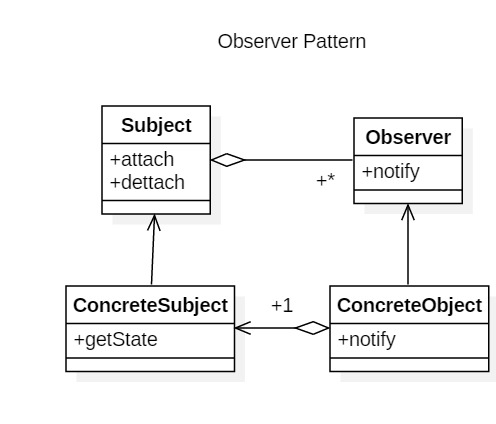
\includegraphics[width=0.6\textwidth]{figures/observer-uml.jpg}
\caption{Observer pattern (UML). A Subject aggregates any number of Observers;
each ConcreteObserver knows its ConcreteSubject so it can call
\code{getState()}.}
\end{figure}

\begin{lstlisting}[style=cpp]
class Observer {
  public:
    virtual void notify() = 0;
    virtual ~Observer() {}
};

class Subject {
    std::vector<Observer*> observers;
  public:
    void attach(Observer *o) { observers.emplace_back(o); }
    void detach(Observer *o) {
        for (auto it = observers.begin(); it != observers.end(); ++it) {
            if (*it == o) { observers.erase(it); break; }
        }
    }
    void notifyObservers() {
        for (auto &o : observers) o->notify();
    }
    virtual ~Subject() = 0;
};
\end{lstlisting}

We want \code{Subject} to be abstract, but it has no obvious pure virtual method
(every subject attaches/detaches/notifies the same way). Trick: make the
\emph{destructor} pure virtual.

\paragraph{Problem.} The dtor of a subclass of \code{Subject} will call the base
class's dtor --- which has no implementation, so the program won't link.

\paragraph{Solution.} Implement \code{Subject}'s dtor anyway:
\begin{lstlisting}[style=cpp]
// subject.cc
Subject::~Subject() {}
\end{lstlisting}
A pure virtual method \emph{may} have an implementation. ``Pure virtual'' means
a subclass must override it to be concrete (for a dtor, every subclass has one
automatically), not that it has no body.

\subsection{Example: A Horse Race}
\begin{lstlisting}[style=cpp]
class HorseRace : public Subject {
    std::ifstream in;          // source of race results
    std::string lastWinner;
  public:
    HorseRace(const std::string &source) : in{source} {}
    bool runRace() { return bool(in >> lastWinner); }
    std::string getState() const { return lastWinner; }
};

class Bettor : public Observer {
    HorseRace *subject;
    std::string name, myHorse;
  public:
    Bettor(HorseRace *hr, const std::string &name, const std::string &horse)
        : subject{hr}, name{name}, myHorse{horse} {
        subject->attach(this);
    }
    ~Bettor() { subject->detach(this); }
    void notify() override {
        std::cout << name
                  << (subject->getState() == myHorse ? " wins!" : " loses.")
                  << std::endl;
    }
};

int main() {
    HorseRace hr{"races.txt"};
    Bettor larry{&hr, "Larry", "RunsLikeACow"};
    Bettor moe{&hr, "Moe", "Molasses"};
    while (hr.runRace()) hr.notifyObservers();
}
\end{lstlisting}
The subject knows nothing about bettors beyond the \code{Observer} interface, so
new kinds of observers can be added without touching \code{HorseRace}.

One round of the race loop, as objects and calls:
\begin{center}
\begin{tikzpicture}[>=Stealth,font=\small,o/.style={draw,rounded corners,fill=green!8,minimum width=2.6cm,minimum height=0.8cm,align=center}]
  \node[draw,rounded corners,fill=blue!6,minimum width=3cm,minimum height=1.2cm,align=center] (hr) at (0,0) {\code{hr}: HorseRace\\ \scriptsize \code{observers} $=$ [\code{\&larry}, \code{\&moe}]};
  \node[o] (l) at (6,1) {\code{larry}: Bettor\\ \scriptsize horse RunsLikeACow};
  \node[o] (m) at (6,-1) {\code{moe}: Bettor\\ \scriptsize horse Molasses};
  \draw[->] ([yshift=4pt]hr.east) -- node[above,sloped,font=\scriptsize]{\code{notify()}} (l.west);
  \draw[->] ([yshift=-4pt]hr.east) -- node[below,sloped,font=\scriptsize]{\code{notify()}} (m.west);
  \draw[->,dashed] (l.north) to[bend right=30] node[above,font=\scriptsize]{\code{subject->getState()}} (hr.north);
  \draw[->,dashed] (m.south) to[bend left=30] node[below,font=\scriptsize]{\code{subject->getState()}} (hr.south);
\end{tikzpicture}
\end{center}

\section{The Decorator Pattern}
We have an object with some behaviour, and while the program is running we want
to add to (enhance) the behaviour of that object. Example: a window, to which we
may add a menu, a scroll bar, a border, \dots{} in any combination.

\begin{figure}[H]
\centering
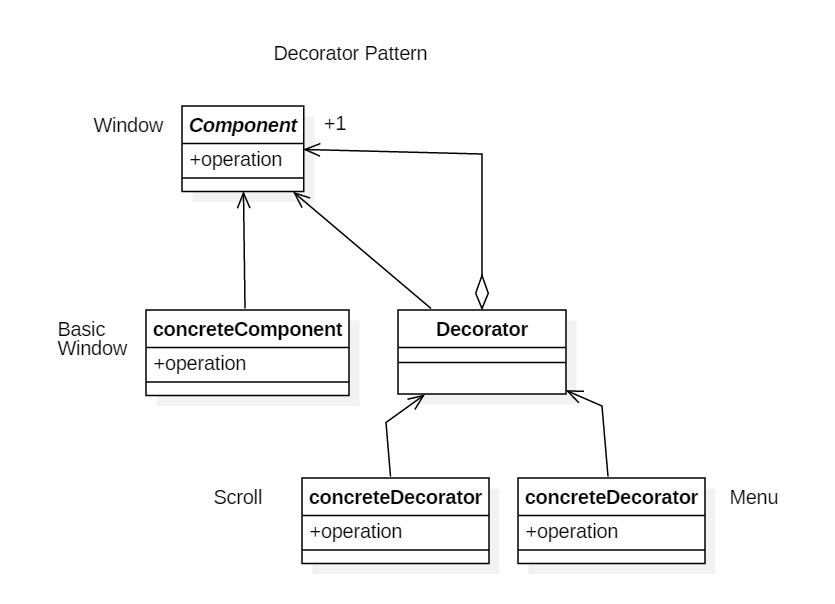
\includegraphics[width=0.75\textwidth]{figures/decorator-uml.jpg}
\caption{Decorator pattern (UML), with the window example: Window is the
abstract component, BasicWindow the concrete component, Scroll and Menu concrete
decorators.}
\end{figure}

\begin{itemize}
  \item \code{Component}: the interface, with the operations to be enhanced.
  \item \code{ConcreteComponent}: the basic object.
  \item \code{Decorator}: an abstract class that \textbf{is-a} Component
        \emph{and} \textbf{has-a} Component (the thing it decorates).
  \item \code{ConcreteDecorator}s: each does its own bit and then delegates to
        the component it wraps.
\end{itemize}
\begin{lstlisting}[style=cpp]
Window *w = new BasicWindow{};
w = new Menu{w};       // a window with a menu
w = new Scroll{w};     // a window with a menu and a scroll bar
w->render();
\end{lstlisting}

\begin{definition}
\textbf{Decorator pattern}: add or enhance behaviour of an existing object at
run time, by wrapping it in objects with the same interface.
\end{definition}

\subsection{Example: Pizza}
\begin{lstlisting}[style=cpp]
class Pizza {                            // Component
  public:
    virtual float price() const = 0;
    virtual std::string desc() const = 0;
    virtual ~Pizza() {}
};

class CrustAndSauce : public Pizza {     // ConcreteComponent
  public:
    float price() const override { return 5.99; }
    std::string desc() const override { return "Pizza"; }
};

class Decorator : public Pizza {         // is-a Pizza
  protected:
    Pizza *component;                    // has-a Pizza
  public:
    Decorator(Pizza *p) : component{p} {}
    virtual ~Decorator() { delete component; }
};

class Topping : public Decorator {
    std::string theTopping;
  public:
    Topping(const std::string &t, Pizza *p) : Decorator{p}, theTopping{t} {}
    float price() const override { return component->price() + 0.75; }
    std::string desc() const override {
        return component->desc() + " with " + theTopping;
    }
};

class StuffedCrust : public Decorator {
  public:
    StuffedCrust(Pizza *p) : Decorator{p} {}
    float price() const override { return component->price() + 2.69; }
    std::string desc() const override {
        return component->desc() + " with stuffed crust";
    }
};

Pizza *p = new CrustAndSauce;
p = new Topping{"cheese", p};
p = new Topping{"mushrooms", p};
p = new StuffedCrust{p};
std::cout << p->desc() << " " << p->price() << std::endl;
// Pizza with cheese with mushrooms with stuffed crust 10.18
delete p;      // deletes the whole chain
\end{lstlisting}
Each decorator owns the component it wraps, so deleting the outermost one frees
everything.

\begin{center}
\begin{tikzpicture}[>=Stealth,font=\small,node distance=0.7cm,
  d/.style={draw,rounded corners,fill=orange!12,minimum height=1cm,align=center,font=\scriptsize},
  c/.style={d,fill=blue!6}]
  \node (p) {\code{p}};
  \node[d,right=0.5cm of p] (s) {StuffedCrust\\ $+2.69$};
  \node[d,right=of s] (m) {Topping\\ mushrooms\\ $+0.75$};
  \node[d,right=of m] (ch) {Topping\\ cheese\\ $+0.75$};
  \node[c,right=of ch] (b) {CrustAndSauce\\ $5.99$};
  \draw[->] (p) -- (s); \draw[->] (s) -- (m);
  \draw[->] (m) -- (ch); \draw[->] (ch) -- (b);
\end{tikzpicture}

\small \code{p->price()} calls inward along the chain and adds on the way back:
$5.99+0.75+0.75+2.69=10.18$.
\end{center}

\section{The Big Five Revisited (with Inheritance)}
\begin{lstlisting}[style=cpp]
class Book {
    ...
  public:
    // defines the Big Five
};
class Text : public Book {
    std::string topic;
  public:
    // does not define the Big Five
};

Text b{"TheFlu", "Nomair", 50, "Medicine"};
Text c = b;     // calls Text's copy ctor
\end{lstlisting}
Remember you get one for free. The free copy ctor of \code{Text} calls Book's
copy ctor on the Book part, then copies the \code{topic} field. Written out, the
free versions are:
\begin{lstlisting}[style=cpp]
// copy ctor
Text::Text(const Text &other) : Book{other}, topic{other.topic} {}

// copy assignment: assign the Book part, then the subclass fields
Text &Text::operator=(const Text &other) {
    Book::operator=(other);
    topic = other.topic;
    return *this;
}
\end{lstlisting}
(\code{Book\{other\}} works because a Text is-a Book: \code{other} binds to
\code{const Book\&}.)

A first (wrong) attempt at the move ctor:
\begin{lstlisting}[style=cpp]
Text::Text(Text &&other) : Book{other}, topic{other.topic} {}   // incorrect
\end{lstlisting}
It won't crash, but it is \emph{copying}, not stealing. (Quick check: if your move
code looks the same as your copy code, it is wrong.)

\begin{aside}
\begin{lstlisting}[style=cpp]
int *p = ...;   // p is a pointer, and p (the variable) is an lvalue
\end{lstlisting}
Likewise, \code{other} has type ``rvalue reference to Text'', but \code{other}
itself is a \emph{named variable}, so it is an \textbf{lvalue}. Hence
\code{Book\{other\}} calls Book's \emph{copy} ctor and \code{topic\{other.topic\}}
calls string's copy ctor.
\end{aside}

We need a way to treat an lvalue as an rvalue: \code{std::move} (from
\code{<utility>}) does exactly that --- it is just a cast to \code{T\&\&}.
\begin{lstlisting}[style=cpp]
Text::Text(Text &&other)
    : Book{std::move(other)}, topic{std::move(other.topic)} {}

Text &Text::operator=(Text &&other) {
    Book::operator=(std::move(other));
    topic = std::move(other.topic);
    return *this;
}
\end{lstlisting}
(Using \code{other.topic} after \code{std::move(other)} is fine: Book's move ctor
only steals the Book part.)

\section{Assignment Through Base Class Pointers}
\begin{lstlisting}[style=cpp]
Text b1{"TheFlu", "Nomair", 50, "Medicine"};
Text b2{"C++IsEasy", "Brad", 500, "CS"};
Book *pb1 = &b1;
Book *pb2 = &b2;
*pb1 = *pb2;     // object assignment through pointers
\end{lstlisting}
\code{Book::operator=} runs (it is non-virtual). Now \code{b1} is
\code{\{"C++IsEasy", "Brad", 500, "Medicine"\}}: only the Book part was assigned.
This is the \textbf{partial assignment problem}.
\begin{center}
\begin{tikzpicture}[>=Stealth,font=\small,f/.style={draw,minimum width=2.4cm,minimum height=0.55cm,font=\scriptsize}]
  \node[font=\scriptsize] at (0,0.55) {\code{b2}};
  \node[f,fill=blue!6] (a1) at (0,0) {C++IsEasy, Brad, 500};
  \node[f,fill=green!10,below=0pt of a1] (a2) {CS};
  \node[font=\scriptsize] at (6,0.55) {\code{b1} afterwards};
  \node[f,fill=blue!6] (b1) at (6,0) {C++IsEasy, Brad, 500};
  \node[f,fill=green!10,below=0pt of b1] (b2) {Medicine};
  \draw[->] (a1) -- node[above,font=\scriptsize]{\code{Book::operator=}} (b1);
  \node[font=\scriptsize,red!60!black,anchor=west] at (b2.east) {\ not copied};
\end{tikzpicture}
\end{center}

\paragraph{Possible solution: make \code{operator=} virtual?}
\begin{lstlisting}[style=cpp]
class Book {
  public:
    virtual Book &operator=(const Book &other);
};
class Text : public Book {
  public:
    Text &operator=(const Text &other) override;  // does not compile:
};                                                // parameter types differ
\end{lstlisting}
To be a valid override, the parameter must be \code{const Book\&}:
\code{Text \&operator=(const Book \&other) override;}. But then \emph{any} Book
can be assigned to a Text: e.g.\ assigning a Comic to a Text through Book
pointers would compile. Not all Books are Texts! This is the \textbf{mixed
assignment problem}.

\paragraph{Alternative: disable assignment through base class pointers.} Make
Book's \code{operator=} non-public:
\begin{itemize}
  \item private? Then subclasses can't call it either (they need it for their
        own \code{operator=}), so it must be \code{protected}.
  \item But Book is not abstract, so then one plain Book could never be assigned
        to another. That says the hierarchy was poorly designed to begin with.
\end{itemize}
The fix (next lecture): an abstract base class with a protected assignment
operator, with plain books as one more concrete subclass.

\section*{Summary}
\begin{itemize}
  \item Observer: Subject keeps a list of \code{Observer*}, notifies them; a pure
        virtual dtor makes a class abstract but still needs a body.
  \item Decorator: is-a and has-a Component; wrap objects to add behaviour at run
        time.
  \item Subclass Big Five must handle the base part (\code{Book\{other\}},
        \code{Book::operator=(other)}).
  \item Inside a move operation the rvalue reference is an lvalue: use
        \code{std::move} to keep moving.
  \item Assigning through base pointers causes partial assignment; a virtual
        \code{operator=} causes mixed assignment.
\end{itemize}

\chapter{Lecture 19: Abstract Base Classes, Factory Method, Template Method, NVI, Maps}
\begin{center}
\textit{March 15, 2018}
\end{center}

\section{Partial and Mixed Assignment: The Fix}
\begin{lstlisting}[style=cpp]
Text a{...}, b{...};
Book *pa{&a};
Book *pb{&b};
*pa = *pb;      // partial assignment
\end{lstlisting}
Making \code{operator=} virtual forces
\code{Text \&Text::operator=(const Book \&)}, which allows mixed assignment.

\paragraph{Solution.} Restructure the hierarchy: make the base class abstract,
give it a \emph{protected} assignment operator, and make each kind of book
(including plain ``normal'' books) a concrete subclass.

\begin{figure}[H]
\centering
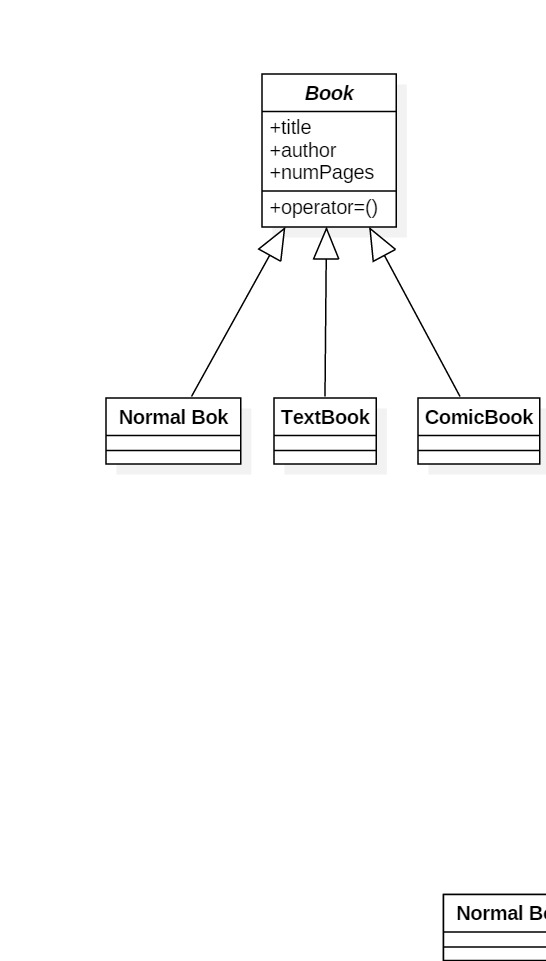
\includegraphics[width=0.5\textwidth, trim=0 480 0 60, clip]{figures/book-uml.jpg}
\caption{Abstract \code{Book} (italic name) with concrete subclasses
\code{NormalBook}, \code{TextBook} and \code{ComicBook}.}
\end{figure}

\begin{lstlisting}[style=cpp]
class AbstractBook {
    std::string title, author;
    int numPages;
  protected:
    AbstractBook &operator=(const AbstractBook &other);  // subclasses only
  public:
    AbstractBook(...);
    virtual ~AbstractBook() = 0;     // abstract; still needs a body
};
AbstractBook::~AbstractBook() {}

class NormalBook : public AbstractBook {
  public:
    NormalBook &operator=(const NormalBook &other) {
        AbstractBook::operator=(other);
        return *this;
    }
};

class Text : public AbstractBook {
    std::string topic;
  public:
    Text &operator=(const Text &other) {
        AbstractBook::operator=(other);
        topic = other.topic;
        return *this;
    }
};
// Comic is similar
\end{lstlisting}
\begin{lstlisting}[style=cpp]
AbstractBook *pa1{&a};
AbstractBook *pb1{&b};
*pa1 = *pb1;    // won't compile: AbstractBook::operator= is protected
a = b;          // fine: Text::operator=, full assignment
\end{lstlisting}
Partial and mixed assignment through base pointers are now both impossible,
while assignment between objects of the same concrete type still works.

\begin{important}[Advice]
In a class hierarchy, make superclasses abstract. (Non-leaf classes should be
abstract.)
\end{important}

\section{The Factory Method Pattern}
Problem: write a video game with two kinds of enemies, turtles and bullets. The
system randomly sends turtles and bullets, but bullets are more frequent in
harder levels. We never know exactly which enemy comes next, so we can't call
the Turtle or Bullet ctor directly; and the decision policy depends on the level.

\begin{lstlisting}[style=cpp]
class Level {
  public:
    virtual Enemy *createEnemy() = 0;   // the factory method
    virtual ~Level() {}
};

class Normal : public Level {
  public:
    Enemy *createEnemy() override {
        // more turtles (they are easier to kill)
    }
};

class Castle : public Level {
  public:
    Enemy *createEnemy() override {
        // more bullets
    }
};

Player *p = ...;
Level *l = new Normal;
Enemy *e = nullptr;
while (p->notDead()) {
    e = l->createEnemy();     // generate an enemy: the level decides which
    // attack the player
}
\end{lstlisting}

Also called the \textbf{Virtual Constructor pattern}: \code{createEnemy} acts
like a constructor whose concrete class is chosen at run time. A related idea:
make a class's constructors private/protected and provide methods that create
objects for the client. We have seen this already: \code{List::addToFront}
creates Nodes; \code{List::begin}/\code{List::end} create Iterators.

\section{The Template Method Pattern}
We want to allow subclasses to override \emph{some} aspects of the superclass's
behaviour, while other aspects must remain the same.

Example: red turtles and green turtles. Drawing a turtle means drawing a head,
a shell and feet; only the shell differs.
\begin{lstlisting}[style=cpp]
class Turtle {
  public:
    void draw() {           // the template method: not virtual
        drawHead();
        drawShell();
        drawFeet();
    }
    virtual ~Turtle() {}
  private:
    void drawHead() { ... }
    void drawFeet() { ... }
    virtual void drawShell() = 0;   // the customizable step
};

class RedTurtle : public Turtle {
    void drawShell() override { /* draw a red shell */ }
};

class GreenTurtle : public Turtle {
    void drawShell() override { /* draw a green shell */ }
};
\end{lstlisting}
Subclasses can't change the overall drawing algorithm (\code{draw} is not
virtual) but they can (must) supply the shell. Note that a subclass may override
a private virtual method, even though it cannot call it.

\section{The Non-Virtual Interface (NVI) Idiom}
Think about what a \textbf{public virtual} method means:
\begin{itemize}
  \item \textbf{public}: the class promises clients a certain, pre-defined
        behaviour (an interface, with pre/post-conditions);
  \item \textbf{virtual}: an invitation to subclasses to change that behaviour
        to anything they like.
\end{itemize}
These pull in opposite directions: we cannot guarantee the behaviour if
subclasses can replace it.

\begin{important}[NVI idiom]
\begin{itemize}
  \item All public methods should be non-virtual (except the destructor).
  \item All virtual methods should be private (or protected, if subclasses need
        to call the base version).
\end{itemize}
\end{important}

\begin{lstlisting}[style=cpp]
class DigitalMedia {         // not following NVI
  public:
    virtual void play() = 0;
    virtual ~DigitalMedia() {}
};

class DigitalMedia {         // using NVI
  public:
    void play() {
        checkCopyright();    // the base class keeps control:
        doPlay();            // e.g. copyright check before, stats after
    }
    virtual ~DigitalMedia() {}
  private:
    void checkCopyright();
    virtual void doPlay() = 0;
};
\end{lstlisting}
With NVI, the base class can later add code before/after every call (logging,
checks) without changing any subclass. It costs nothing (\code{play} can be
inlined), so the advice is to always use it. It generalizes the Template Method
pattern: every virtual method is wrapped in a non-virtual template method.

\section{The STL \code{map}}
A \code{map} is a generalization of an array where the key (index) and the value
can be of any type (the key type must support \code{operator<}, since maps are
kept sorted --- typically as balanced binary search trees). It is a template
class parameterized on two types.
\begin{lstlisting}[style=cpp]
#include <map>
...
map<string, int> m;
m["abc"] = 1;
m["def"] = 4;
cout << m["abc"] << endl;   // prints 1
cout << m["ghi"] << endl;   // prints 0: if the key is absent, operator[]
                            // default-constructs a value and inserts it!

if (m.count("def")) { ... } // lookup without inserting:
                            // 0 if no such key, 1 if found
m.erase("abc");
\end{lstlisting}
Another STL class, \code{multimap}, allows several values per key --- look at it
on your own time.

Surprise, surprise: an iterator is predefined.
\begin{lstlisting}[style=cpp]
for (auto &p : m) {
    // p has type std::pair<const string, int> (a struct in the STL)
    cout << p.first << " " << p.second << endl;   // fields, not methods
}
\end{lstlisting}
Iteration happens in sorted key order.

\section{The Visitor Pattern: Double Dispatch}
The Visitor pattern is used for \textbf{double dispatch}: choosing which method to
call based on the run-time types of \emph{two} objects.

Example: enemies and weapons. The effect of striking depends on both the kind of
enemy and the kind of weapon.
\begin{quote}
\textit{``Enenemy --- that's not how you spell enemy.''} --- Nomair
\end{quote}
\begin{lstlisting}[style=cpp]
class Enemy {
  public:
    virtual void strike(Rock &) = 0;
    virtual void strike(Stick &) = 0;
};
\end{lstlisting}
This assumes we know the exact type of the weapon at compile time. Gameplay
doesn't look like that:
\begin{lstlisting}[style=cpp]
Enemy *e = l->createEnemy();
Weapon *w = p->chooseWeapon();
e->strike(*w);      // which strike? *w is only known to be a Weapon
\end{lstlisting}
C++ dynamically dispatches on the object a method is called on, but not on the
argument types (overloading is resolved at compile time).

The Visitor pattern is a clever combination of overriding and overloading:
\begin{lstlisting}[style=cpp]
class Enemy {
  public:
    virtual void strike(Weapon &w) = 0;
    virtual ~Enemy() {}
};

class Turtle : public Enemy {
  public:
    void strike(Weapon &w) override { w.useOn(*this); }  // *this is a Turtle
};
class Bullet : public Enemy {
  public:
    void strike(Weapon &w) override { w.useOn(*this); }  // *this is a Bullet
};

class Weapon {
  public:
    virtual void useOn(Turtle &t) = 0;
    virtual void useOn(Bullet &b) = 0;
    virtual ~Weapon() {}
};

class Stick : public Weapon {
  public:
    void useOn(Turtle &t) override { /* stick on turtle */ }
    void useOn(Bullet &b) override { /* stick on bullet */ }
};
class Rock : public Weapon {
  public:
    void useOn(Turtle &t) override { /* rock on turtle */ }
    void useOn(Bullet &b) override { /* rock on bullet */ }
};
\end{lstlisting}
The two \code{strike} bodies look identical, but putting them in \code{Enemy}
to reuse code would be wrong: the whole point is that inside \code{Turtle}, the
type of \code{*this} is known to be \code{Turtle}, which selects the right
overload of \code{useOn}.

\begin{lstlisting}[style=cpp]
Enemy *e = ...;   // suppose it is a Turtle
Weapon *w = ...;  // suppose it is a Stick
e->strike(*w);
\end{lstlisting}
\begin{enumerate}
  \item \code{strike} is virtual: \code{Turtle::strike} runs (dispatch on the
        enemy);
  \item it calls \code{w.useOn(*this)} with \code{*this} of static type
        \code{Turtle\&}: overload resolution picks \code{useOn(Turtle\&)};
  \item \code{useOn} is virtual: \code{Stick::useOn(Turtle\&)} runs (dispatch on
        the weapon).
\end{enumerate}
More uses of Visitor next lecture.

\section*{Summary}
\begin{itemize}
  \item Fix partial/mixed assignment with an abstract base class whose
        \code{operator=} is protected; make non-leaf classes abstract.
  \item Factory Method: a virtual method creates objects whose concrete type the
        subclass decides.
  \item Template Method: a non-virtual algorithm calls virtual steps.
  \item NVI: public methods non-virtual, virtual methods private.
  \item \code{map<K,V>}: \code{operator[]} inserts defaults; use \code{count} to
        test membership; iteration yields sorted \code{pair}s.
  \item Visitor: \code{strike} (override) + \code{useOn(*this)} (overload) gives
        double dispatch.
\end{itemize}

\chapter{Lecture 20: Visitor Continued, Compilation Dependencies and Pimpl}
\begin{center}
\textit{March 20, 2018}
\end{center}

\begin{aside}
The original notes for this lecture are missing; this chapter reconstructs it
from the course order (Visitor in Lecture 19, exception safety in Lecture 21)
and the standard CS 246 sequence of that term.
\end{aside}

\section{Visitor Recap}
Last time: double dispatch.
\begin{lstlisting}[style=cpp]
e->strike(*w);
// 1. virtual Enemy::strike   -> chooses on the enemy's run-time type
// 2. w.useOn(*this)          -> overload chosen by the static type of *this
// 3. virtual Weapon::useOn   -> chooses on the weapon's run-time type
\end{lstlisting}

\section{Visitor, Second Use: Adding Operations to a Hierarchy}
The Visitor pattern can also be used to add functionality to an existing class
hierarchy \emph{without} adding new virtual methods to every class.

Suppose we want to do something with our Book hierarchy that its designers did
not anticipate --- e.g.\ build a catalogue: count Books by author, Texts by
topic, Comics by hero. Each new operation would normally mean a new virtual
method in \code{Book}, \code{Text} and \code{Comic}. Instead, add a single
\code{accept} method once, and let \emph{visitors} supply the operations:
\begin{lstlisting}[style=cpp]
class BookVisitor {
  public:
    virtual void visit(Book &b) = 0;
    virtual void visit(Text &t) = 0;
    virtual void visit(Comic &c) = 0;
    virtual ~BookVisitor() {}
};

class Book {
  public:
    virtual void accept(BookVisitor &v) { v.visit(*this); }
    virtual ~Book() {}
    ...
};
class Text : public Book {
  public:
    void accept(BookVisitor &v) override { v.visit(*this); }
    ...
};
class Comic : public Book {
  public:
    void accept(BookVisitor &v) override { v.visit(*this); }
    ...
};
\end{lstlisting}
(\code{accept} plays the role of \code{strike}; \code{visit} plays the role of
\code{useOn}.)

A visitor that builds the catalogue:
\begin{lstlisting}[style=cpp]
class Catalogue : public BookVisitor {
    std::map<std::string, int> theCatalogue;
  public:
    std::map<std::string, int> getCatalogue() const { return theCatalogue; }
    void visit(Book &b) override { ++theCatalogue[b.getAuthor()]; }
    void visit(Text &t) override { ++theCatalogue[t.getTopic()]; }
    void visit(Comic &c) override { ++theCatalogue[c.getHero()]; }
};

std::vector<Book*> collection{...};
Catalogue cat;
for (auto b : collection) b->accept(cat);
for (auto &p : cat.getCatalogue())
    std::cout << p.first << ": " << p.second << std::endl;
\end{lstlisting}
Recall that \code{m[key]} inserts \code{0} for a missing key, so
\code{++theCatalogue[...]} counts correctly from zero.

Any further operation (e.g.\ total pages per category, printing a report) is
just another \code{BookVisitor} subclass; \code{Book}, \code{Text} and
\code{Comic} are untouched.

\begin{important}[Trade-off of Visitor]
Visitor makes it easy to add new \emph{operations}, but hard to add new
\emph{classes} to the visited hierarchy: a new Book subclass requires a new
\code{visit} overload in \code{BookVisitor} and in every visitor.
\end{important}

\section{Compilation Dependencies}
Visitor creates a lot of mutual dependencies: \code{book.h} mentions
\code{BookVisitor}, and \code{bookvisitor.h} mentions \code{Book}, \code{Text}
and \code{Comic}. If each header \code{\#include}s the other we get an include
cycle, and the include guards cause one of the files to see an undefined class.

\paragraph{Q.} When do we need \code{\#include "a.h"}, and when does a
\textbf{forward declaration} \code{class A;} suffice?

The compiler needs the full definition of a class when it needs to know the
class's \emph{size} or its \emph{members}:
\begin{lstlisting}[style=cpp]
// a.h
class A { ... };

// b.h
#include "a.h"
class B : public A { ... };      // inheritance: needs A's size and members

// c.h
#include "a.h"
class C {
    A myA;                       // a field of type A: needs A's size
};

// d.h
class A;                         // forward declaration is enough
class D {
    A *myAp;                     // pointers all have the same size
};

// e.h
class A;
class E {
    A f(A x);                    // only a declaration: no size needed yet
};
\end{lstlisting}
In the implementation files, D and E will need the full definition of A
(\code{d.cc} dereferences the pointer; \code{e.cc} actually passes and returns
A's), so \code{d.cc} and \code{e.cc} \code{\#include "a.h"}.

\begin{important}[Advice]
Do not \code{\#include} a header when a forward declaration suffices. Prefer
forward declarations in headers and includes in \code{.cc} files.
\end{important}
Why bother?
\begin{itemize}
  \item it breaks include cycles;
  \item it reduces compilation dependencies: if \code{a.h} changes, only files
        that really include it are recompiled (\code{make} with \code{-MMD}
        follows the includes). Large projects can take hours to build, so this
        matters.
\end{itemize}

\section{The Pimpl Idiom}
Even a private field creates a compilation dependency:
\begin{lstlisting}[style=cpp]
// window.h
#include <X11/Xlib.h>
class XWindow {
    Display *d;
    Window w;
    int s;
    GC gc;
    unsigned long colours[10];
  public:
    ...
};
\end{lstlisting}
Every client that includes \code{window.h} also includes the whole X11 header,
and must be recompiled whenever a \emph{private} field of \code{XWindow} is added
or changed --- even though clients can't use those fields.

\begin{definition}
\textbf{Pimpl} (``pointer to implementation''): move all private fields into a
separate implementation struct, defined only in the \code{.cc} file, and store
only a pointer to it in the class.
\end{definition}

\begin{lstlisting}[style=cpp]
// window.h
struct XWindowImpl;              // forward declaration only
class XWindow {
    XWindowImpl *pImpl;
  public:
    XWindow();
    ~XWindow();
    ...                          // no change to the public interface
};

// windowimpl.h
#include <X11/Xlib.h>
struct XWindowImpl {
    Display *d;
    Window w;
    int s;
    GC gc;
    unsigned long colours[10];
};

// window.cc
#include "window.h"
#include "windowimpl.h"
XWindow::XWindow() : pImpl{new XWindowImpl} { ... }
XWindow::~XWindow() { delete pImpl; }
// other methods use pImpl->d, pImpl->w, ... instead of d, w, ...
\end{lstlisting}
Now clients include only \code{window.h}, which does not include X11. If the
implementation struct changes, only \code{window.cc} is recompiled; clients just
re-link. (Since the class now owns heap memory, the Rule of Five applies; with a
smart pointer from Lecture~21, \code{std::unique\_ptr<XWindowImpl>}, most of it
is automatic.)

\section{The Bridge Pattern}
Taking Pimpl further: if there are several possible window implementations
(X11, a Windows API, a test stub), make the implementation struct a
\emph{polymorphic class hierarchy}:
\begin{lstlisting}[style=cpp]
class WindowImpl {               // abstract implementation interface
  public:
    virtual void drawPixel(int x, int y, int colour) = 0;
    virtual ~WindowImpl() {}
};
class XWindowImpl : public WindowImpl { ... };
class MSWindowImpl : public WindowImpl { ... };

class Window {                   // abstraction
    WindowImpl *pImpl;           // chosen at construction time
  public:
    void fillRectangle(int x, int y, int w, int h, int colour);  // uses pImpl
};
\end{lstlisting}

\begin{center}
\begin{tikzpicture}[cls/.style={draw, minimum width=22mm, minimum height=8mm,
  font=\small}]
\node[cls] (w) {Window};
\node[cls, right=30mm of w] (wi) {\textit{WindowImpl}};
\node[cls, below left=12mm and -8mm of wi] (x) {XWindowImpl};
\node[cls, below right=12mm and -8mm of wi] (m) {MSWindowImpl};
\draw[-{Diamond[fill=black,length=4mm,width=2.5mm]}] (wi) -- (w);
\draw[-{Triangle[open,length=3mm,width=3mm]}] (x.north) -- (wi.south west);
\draw[-{Triangle[open,length=3mm,width=3mm]}] (m.north) -- (wi.south east);
\end{tikzpicture}
\end{center}

\begin{definition}
\textbf{Bridge pattern}: separate an abstraction from its implementation so the
two can vary independently --- new kinds of windows (subclassing
\code{Window}) and new platforms (subclassing \code{WindowImpl}) can each be
added without touching the other hierarchy.
\end{definition}

\section*{Summary}
\begin{itemize}
  \item Visitor also adds operations to a hierarchy: one \code{accept} per class,
        one visitor class per operation. Easy to add operations, hard to add
        classes.
  \item Include a header only when you need a class's size or members; otherwise
        forward-declare. This breaks cycles and speeds up rebuilds.
  \item Pimpl hides private fields behind a pointer to an implementation struct,
        so clients don't recompile when the implementation changes.
  \item Bridge: Pimpl with a polymorphic implementation hierarchy.
\end{itemize}

\chapter{Lecture 21: Exception Safety, RAII and Smart Pointers}
\begin{center}
\textit{March 22, 2018}
\end{center}

\section{The Problem}
\begin{lstlisting}[style=cpp]
void f() {
    MyClass *p = new MyClass;
    MyClass mc;
    g();
    delete p;
}
\end{lstlisting}
Suppose \code{g} itself does not leak memory. Still, if \code{g} throws an
exception, \code{delete p} is never executed: \code{f} leaks memory.

We want to write \textbf{exception-safe} code. (This does \emph{not} mean ``code
that doesn't use exceptions''.) Exceptions are meant to be recovered from, so an
exception should not leave behind
\begin{itemize}
  \item memory leaks,
  \item dangling pointers,
  \item broken class invariants.
\end{itemize}

\begin{important}[C++ guarantee]
During stack unwinding, all stack-allocated objects are destroyed: their
destructors run and their memory is reclaimed. Nothing is promised about heap
memory.
\end{important}
So in \code{f}, \code{mc} is cleaned up, but the object \code{p} points to leaks.
A pointer is just a value: destroying \code{p} does not (and should not, on its
own) call \code{delete} on it.

\section{Refactoring by Hand}
\begin{lstlisting}[style=cpp]
void f() {
    MyClass *p = new MyClass;
    try {
        MyClass mc;
        g();
    } catch (...) {
        delete p;
        throw;          // re-throw: we only cleaned up
    }
    delete p;
}
\end{lstlisting}
This is tedious and error-prone (note the duplicated cleanup, and imagine five
pointers). We would like the ability to run some code no matter whether an
exception occurred:
\begin{itemize}
  \item Java has \code{finally};
  \item Scheme has \code{dynamic-wind}.
\end{itemize}
C++ has neither --- and doesn't need one, because of the guarantee above: the
only code guaranteed to run during unwinding is the destructors of stack
objects. So:
\begin{enumerate}
  \item maximize your use of the stack;
  \item but what if you really do need the heap?
\end{enumerate}

\section{RAII}
\begin{definition}
\textbf{RAII} --- \emph{Resource Acquisition Is Initialization} (a C++ idiom
named by Bjarne Stroustrup): every resource should be wrapped inside a
stack-allocated object whose destructor's job is to release the resource.
\end{definition}
We have been using it since the second C++ lecture:
\begin{lstlisting}[style=cpp]
{
    ifstream f{"hello.txt"};   // file is opened (acquired) at initialization
    ...
}                              // f's dtor runs: the file is closed (released)
\end{lstlisting}
The file is closed whether the block ends normally or by an exception.

Heap memory is a resource! Idea: wrap the heap object inside a stack object,
whose destructor deletes the heap object.

\section{\code{std::unique\_ptr}}
The standard library (\code{<memory>}) provides the template class
\code{std::unique\_ptr<T>}:
\begin{itemize}
  \item its ctor takes a \code{T*};
  \item its dtor calls \code{delete} on that pointer;
  \item it overloads \code{*} and \code{->}, so it can be used exactly like
        the raw pointer to the heap object.
\end{itemize}
\begin{lstlisting}[style=cpp]
#include <memory>

void f() {
    std::unique_ptr<MyClass> p{new MyClass};
    MyClass mc;
    g();
}   // no leak, whether or not g throws
\end{lstlisting}
Better: use \code{std::make\_unique}, which allocates the object and passes its
arguments to the \code{MyClass} ctor:
\begin{lstlisting}[style=cpp]
auto p = std::make_unique<MyClass>(/* args to MyClass ctor, if any */);
\end{lstlisting}

What about copying?
\begin{lstlisting}[style=cpp]
unique_ptr<C> p{new C};      // or: auto p = make_unique<C>();
unique_ptr<C> q = p;         // won't compile
\end{lstlisting}
If both \code{p} and \code{q} pointed to the object, it would be deleted twice.
So copying is disabled for \code{unique\_ptr}; moving still works (stealing is
still acceptable in C++ society):
\begin{lstlisting}[style=cpp]
unique_ptr<C> q = std::move(p);   // q owns the object; p is now null
\end{lstlisting}

\subsection{A Basic Implementation}
\begin{lstlisting}[style=cpp]
template <typename T> class unique_ptr {
    T *ptr;
  public:
    explicit unique_ptr(T *p) : ptr{p} {}
    ~unique_ptr() { delete ptr; }

    unique_ptr(const unique_ptr &other) = delete;              // no copy ctor
    unique_ptr &operator=(const unique_ptr &other) = delete;   // no copy assign

    unique_ptr(unique_ptr &&other) : ptr{other.ptr} {          // move ctor
        other.ptr = nullptr;
    }
    unique_ptr &operator=(unique_ptr &&other) {                // move assign
        using std::swap;
        swap(ptr, other.ptr);
        return *this;
    }

    T &operator*() const { return *ptr; }
    T *operator->() const { return ptr; }
    T *get() const { return ptr; }
};
\end{lstlisting}
\code{= delete} explicitly removes a function the compiler would otherwise
provide for free. (Note the move operations take \code{unique\_ptr\&\&}, not
\code{const unique\_ptr\&\&}: we must modify \code{other} to steal from it.)

\subsection{Ownership}
With smart pointers, the type of a pointer documents ownership:
\begin{itemize}
  \item \code{unique\_ptr<T>}: \textbf{owns} the object (responsible for deleting
        it). Composition (owns-a) relationships use \code{unique\_ptr} fields ---
        and then the class needs no hand-written destructor.
  \item raw pointer \code{T*}: \textbf{does not own}, just observes.
        Aggregation (has-a) relationships use raw pointers (or references). Get
        one from a \code{unique\_ptr} with \code{p.get()}.
  \item Never call \code{delete} on a raw pointer in a program that uses smart
        pointers for ownership.
\end{itemize}

\section{\code{std::shared\_ptr}}
Sometimes there is no single owner: several objects legitimately share one heap
object, and it should be deleted when the \emph{last} of them is done with it.
\begin{lstlisting}[style=cpp]
void f() {
    auto p1 = std::make_shared<C>();
    if (...) {
        auto p2 = p1;   // copy ctor: p1 and p2 point to the same heap object
        ...
    }                   // p2 goes out of scope: dtor runs, object NOT deleted
    ...
}                       // p1 goes out of scope: dtor runs, object deleted
\end{lstlisting}
Shared pointers use \textbf{reference counting}: a counter (stored on the heap
next to the object) records how many \code{shared\_ptr}s point to the same
object. Copying increments the count; destroying (or reassigning) a
\code{shared\_ptr} decrements it; when the count reaches 0 the object is deleted.

\begin{important}[Caveats]
\begin{itemize}
  \item Reference counting costs time and space; prefer \code{unique\_ptr} unless
        ownership really is shared.
  \item \textbf{Cycles}: if A holds a \code{shared\_ptr} to B and B holds a
        \code{shared\_ptr} to A, neither count ever reaches 0 and both leak.
        Break cycles by making one direction a non-owning pointer (raw pointer or
        \code{std::weak\_ptr}, which observes without contributing to the count).
  \item Never create two separate \code{shared\_ptr}s from the same raw pointer
        (\code{shared\_ptr<C> a\{p\}, b\{p\};}): they keep separate counts and
        both delete \code{p}. Use \code{make\_shared}, and copy the
        \code{shared\_ptr} itself.
\end{itemize}
\end{important}

\section*{Summary}
\begin{itemize}
  \item Exception safety: no leaks, dangling pointers or broken invariants when
        an exception passes through.
  \item C++ only guarantees that stack objects are destroyed during unwinding,
        so wrap every resource in a stack object (RAII).
  \item \code{unique\_ptr}: sole owner, move-only; create with
        \code{make\_unique}.
  \item \code{shared\_ptr}: shared ownership via reference counting; create with
        \code{make\_shared}; beware cycles.
  \item Raw pointers are for non-owning access.
\end{itemize}

\chapter{Topic: Exception Safety Guarantees}

\begin{aside}
This chapter continues Lecture 21 and covers material from the remainder of the
term (not in the original lecture notes).
\end{aside}

\section{Levels of Exception Safety}
Lecture 21 made sure resources are released when an exception passes through. But
what state is an object left in? There are three standard levels of guarantee a
function can offer:

\begin{definition}
\begin{enumerate}
  \item \textbf{Basic guarantee}: if an exception occurs, the program is in
        \emph{some} valid but unspecified state. Nothing is leaked, no
        invariants are broken.
  \item \textbf{Strong guarantee}: if an exception is raised while executing
        \code{f}, the state of the program is as if \code{f} had not been
        called (``commit or roll back'').
  \item \textbf{No-throw guarantee}: \code{f} never throws an exception, and
        always accomplishes its task.
\end{enumerate}
\end{definition}
A function that gives none of these is not exception safe at all.

\section{An Example}
\begin{lstlisting}[style=cpp]
class A { ... };
class B { ... };
class C {
    A a;
    B b;
  public:
    void f() {
        a.g();   // may throw (strong guarantee)
        b.h();   // may throw (strong guarantee)
    }
};
\end{lstlisting}
Is \code{C::f} exception safe?
\begin{itemize}
  \item If \code{a.g()} throws: nothing has happened yet (\code{g} has the
        strong guarantee). OK.
  \item If \code{b.h()} throws: the effects of \code{h} are undone, but
        \code{a.g()} has already happened and is not undone. So \code{f} would
        need to undo \code{g}'s effects --- very hard or impossible if \code{g}
        had non-local side effects (printing, writing a file).
\end{itemize}
So \code{f} offers only the basic guarantee (at best).

\subsection{Achieving the Strong Guarantee}
If \code{A::g} and \code{B::h} have no non-local side effects, we can do the
work on \emph{copies} and then swap them in:
\begin{lstlisting}[style=cpp]
class C {
    A a;
    B b;
  public:
    void f() {
        A atemp = a;    // may throw: fine, nothing changed yet
        B btemp = b;
        atemp.g();      // may throw: fine, only the copies changed
        btemp.h();
        a = atemp;      // what if copy assignment throws?
        b = btemp;
    }
};
\end{lstlisting}
The last two lines are the problem: if \code{b = btemp} throws, \code{a} has
already been modified. We need the ``commit'' step to be no-throw. Assigning
\emph{pointers} can't throw --- so use the pImpl idiom:
\begin{lstlisting}[style=cpp]
struct CImpl {
    A a;
    B b;
};

class C {
    std::unique_ptr<CImpl> pImpl;
  public:
    void f() {
        auto temp = std::make_unique<CImpl>(*pImpl);  // copy: may throw, fine
        temp->a.g();                                  // may throw, fine
        temp->b.h();                                  // may throw, fine
        std::swap(pImpl, temp);                       // no-throw commit
    }   // temp (the old state) is destroyed here
};
\end{lstlisting}
Now \code{f} has the strong guarantee (assuming \code{g} and \code{h} have no
non-local side effects). This is the same idea as copy-and-swap for
\code{operator=}.
\begin{center}
\begin{tikzpicture}[>=Stealth,font=\small,c/.style={draw,fill=blue!5,minimum width=1.4cm,minimum height=0.65cm}]
  \node[c] (pi) at (0,0) {\code{pImpl}};
  \node[c] (t) at (0,-1.2) {\code{temp}};
  \node[draw,fill=gray!12,minimum width=2.2cm,minimum height=0.7cm] (old) at (3.6,0) {old \code{a}, \code{b}};
  \node[draw,fill=green!12,minimum width=2.2cm,minimum height=0.7cm] (new) at (3.6,-1.2) {modified copy};
  \draw[->] (pi) -- (old); \draw[->] (t) -- (new);
  \draw[<->,thick,blue!60!black] (-0.9,0) to[bend right=40] node[left,font=\scriptsize]{\code{swap}} (-0.9,-1.2);
  \node[font=\scriptsize,align=left,anchor=west] at (5.0,-0.6) {all throwing work happens on the copy;\\ the swap of two pointers cannot throw};
\end{tikzpicture}
\end{center}

\begin{important}[Rule of thumb]
Do everything that might throw on the side (on copies/temporaries), then commit
with operations that cannot throw (pointer assignment, swap of built-in types,
moves marked \code{noexcept}).
\end{important}

\section{Exception Safety and \code{vector}}
\code{vector} manages a heap array with RAII: when a vector goes out of scope,
its dtor frees the array and calls the dtor of every element.

\begin{itemize}
  \item \code{vector<C>}: owns the \code{C} objects; they are destroyed with
        the vector.
  \item \code{vector<C*>}: the dtor frees the array of pointers, but does
        \emph{not} delete the objects pointed to (pointers have no dtor). If the
        vector should own them, you must delete them yourself:
\begin{lstlisting}[style=cpp]
for (auto p : v) delete p;
\end{lstlisting}
  \item \code{vector<unique\_ptr<C>>}: owns the objects, and frees them
        automatically, even during unwinding. No explicit cleanup loop needed.
\end{itemize}

\subsection{\code{emplace\_back} and \code{noexcept}}
\code{vector::emplace\_back} (and \code{push\_back}) offer the strong guarantee:
if it throws, the vector is unchanged. When the array is full, it must
\begin{enumerate}
  \item allocate a bigger array,
  \item copy the elements from the old array to the new one,
  \item delete the old array.
\end{enumerate}
If a copy throws midway (step 2), the new array is simply discarded and the old
one is intact: strong guarantee.

But copying is expensive; moving would be much faster. However, if a \emph{move}
throws midway, some elements of the old array have already been gutted, and the
original state can't be restored. So \code{vector} only moves elements if the
move ctor is guaranteed not to throw; otherwise it copies.
\begin{center}
\begin{tikzpicture}[>=Stealth,font=\small,x=0.8cm,c/.style={draw,minimum width=0.8cm,minimum height=0.6cm}]
  \node[anchor=east,font=\scriptsize] at (-0.6,0) {old array (full)};
  \foreach \k in {0,...,3} \node[c,fill=gray!12] (o\k) at (\k,0) {$e_\k$};
  \node[anchor=east,font=\scriptsize] at (-0.6,-1.4) {new array};
  \foreach \k in {0,...,3} \node[c,fill=green!10] (n\k) at (\k,-1.4) {$e_\k$};
  \foreach \k in {4,...,7} \node[c] at (\k,-1.4) {};
  \foreach \k in {0,...,3} \draw[->] (o\k) -- (n\k);
  \node[font=\scriptsize,anchor=west,align=left] at (4.4,0) {copied, or moved if the move ctor\\ is \code{noexcept}; then the old array is freed};
\end{tikzpicture}
\end{center}

\begin{important}[Advice]
Declare move constructors and move assignment operators (and \code{swap}) as
\code{noexcept} when they cannot throw --- which is almost always.
\begin{lstlisting}[style=cpp]
class C {
  public:
    C(C &&other) noexcept;
    C &operator=(C &&other) noexcept;
};
\end{lstlisting}
Otherwise \code{vector} (and other library code) will silently fall back to the
slower copy. Destructors are implicitly \code{noexcept}.
\end{important}

\section{Exception-Safe \code{operator=}}
Compare the versions of \code{Node::operator=} from Lectures 10--11:
\begin{center}
\begin{tabular}{@{}lp{0.55\textwidth}@{}}
\toprule
Version & Guarantee \\
\midrule
\code{delete next;} then \code{new} & none: leaves a dangling \code{next} if
\code{new} throws \\
\code{new} into temp, then \code{delete} old & strong \\
copy-and-swap & strong (if the copy ctor is safe and \code{swap} is no-throw) \\
\bottomrule
\end{tabular}
\end{center}

\section*{Summary}
\begin{itemize}
  \item Basic: valid state, no leaks. Strong: all-or-nothing. No-throw: never
        fails.
  \item A sequence of strong operations is not automatically strong.
  \item Achieve strong guarantee by working on copies and committing with
        no-throw operations (pImpl + swap).
  \item Use \code{vector<unique\_ptr<C>>} for owned polymorphic objects.
  \item Mark moves and swaps \code{noexcept} so containers can use them.
\end{itemize}

\chapter{Topic: Coupling, Cohesion and MVC}

\begin{aside}
Material from the remainder of the term, not covered in the original lecture
notes.
\end{aside}

\section{Measures of Design Quality}
How do we tell whether a modular design is good? Two classic measures.

\subsection{Coupling}
\begin{definition}
\textbf{Coupling} is how much distinct modules (classes) depend on each other.
\end{definition}
From low (good) to high (bad):
\begin{enumerate}
  \item modules communicate via function calls with basic parameters/results;
  \item modules pass arrays/structs back and forth;
  \item modules affect each other's control flow (e.g.\ passing flags that tell
        the other module what to do);
  \item modules share global data;
  \item modules have access to each other's implementation (\code{friend}s,
        public fields).
\end{enumerate}
With high coupling, changes to one module require changes to others, and modules
are hard to reuse individually.

\subsection{Cohesion}
\begin{definition}
\textbf{Cohesion} is how closely the elements of a single module are related to
each other.
\end{definition}
From low (bad) to high (good):
\begin{enumerate}
  \item arbitrary grouping of unrelated elements (e.g.\ \code{<utility>}:
        \code{swap}, \code{pair}, \code{move}, \dots);
  \item elements share a common theme but are otherwise unrelated, maybe sharing
        some base code (e.g.\ \code{<algorithm>});
  \item elements manipulate the same state over the lifetime of an object (e.g.\
        open/read/close a file);
  \item elements pass data to each other (a pipeline);
  \item elements cooperate to perform exactly one task.
\end{enumerate}
With low cohesion, modules are poorly organized and hard to understand and
maintain.

\begin{important}[Goal]
Low coupling, high cohesion.
\end{important}

\section{Decoupling the Interface}
Your primary program classes should not be printing things. Consider
\begin{lstlisting}[style=cpp]
class ChessBoard {
    ...
    void move(...) {
        ...
        std::cout << "Your move" << std::endl;
    }
};
\end{lstlisting}
This is bad design: it inhibits code reuse. What if we want a graphical display,
or to use the same game logic over the network, or to write output to a file?
Slightly better: give the class a stream to print to,
\begin{lstlisting}[style=cpp]
class ChessBoard {
    std::ostream &out;
  public:
    ChessBoard(std::ostream &out) : out{out} {}
    ...
};
\end{lstlisting}
but it still assumes a text interface.

\begin{definition}
\textbf{Single Responsibility Principle}: a class should have only one reason to
change.
\end{definition}
If two distinct parts of the specification can change independently (the rules
of chess vs.\ how the board is displayed), they belong in different classes.
\code{ChessBoard} should communicate with its user via parameters, results, and
possibly exceptions; a separate class handles I/O.

\section{Model--View--Controller (MVC)}
\begin{definition}
\textbf{MVC} separates a program into three parts:
\begin{itemize}
  \item the \textbf{model}: the main data and logic you are manipulating (e.g.\
        the game state);
  \item the \textbf{view}: how the model is displayed;
  \item the \textbf{controller}: how the model is manipulated (interprets user
        input, decides what to do).
\end{itemize}
\end{definition}

\begin{center}
\begin{tikzpicture}[cls/.style={draw, minimum width=24mm, minimum height=9mm},
  >={Stealth}]
\node[cls] (m) {Model};
\node[cls, below left=15mm and 6mm of m] (v) {View};
\node[cls, below right=15mm and 6mm of m] (c) {Controller};
\draw[->] (c) -- node[right, font=\small] {updates} (m);
\draw[->, dashed] (m) -- node[left, font=\small] {notifies} (v);
\draw[->] (v) -- node[below, font=\small] {user input} (c);
\end{tikzpicture}
\end{center}

\begin{itemize}
  \item The model may have multiple views (text and graphics at the same time).
        It doesn't need to know their details: the model is typically a
        \textbf{subject} and the views are \textbf{observers} (Observer pattern,
        Lecture 18).
  \item The controller mediates control flow between model and view. The model
        may (or may not) hold a reference to the controller.
  \item Swapping out the view or controller does not require changing the model,
        and the model can be tested without any UI.
\end{itemize}

\begin{lstlisting}[style=cpp]
class Game : public Subject {          // model
    Board board;
  public:
    bool makeMove(const Move &m);      // returns false if illegal
    const Board &getState() const { return board; }
};

class TextDisplay : public Observer {  // view
    Game &game;
    std::ostream &out;
  public:
    TextDisplay(Game &g, std::ostream &out) : game{g}, out{out} {
        game.attach(this);
    }
    void notify() override { out << game.getState(); }
};

class Controller {                     // controller
    Game &game;
  public:
    explicit Controller(Game &g) : game{g} {}
    void play(std::istream &in) {
        Move m;
        while (in >> m) {
            if (game.makeMove(m)) game.notifyObservers();
            else std::cerr << "Illegal move" << std::endl;
        }
    }
};
\end{lstlisting}

\section{Other Design Principles}
\begin{itemize}
  \item \textbf{Open/Closed Principle}: classes should be open for extension
        but closed for modification. Changes in a program should happen by
        writing \emph{new} code (new subclasses, new decorators, new visitors),
        not by editing working code. Strategies, Decorator, Template Method and
        Visitor all support this.
  \item \textbf{Liskov Substitution Principle}: if B is a subtype of A, a B must
        be usable anywhere an A is expected, without the client noticing.
        Subclasses must not strengthen preconditions, weaken postconditions or
        break invariants of the superclass. (Classic violation: \code{Square} as
        a subclass of a mutable \code{Rectangle} --- setting the width of a
        square also changes its height, which no Rectangle client expects.)
  \item \textbf{Program to an interface} (Lecture 17), and prefer composition
        over inheritance when the relationship is not really is-a.
\end{itemize}

\section*{Summary}
\begin{itemize}
  \item Aim for low coupling (modules depend on each other as little as
        possible) and high cohesion (each module does one coherent thing).
  \item Keep I/O out of core logic (Single Responsibility).
  \item MVC: model (data/logic, a Subject), views (Observers that display it),
        controller (turns input into model operations).
  \item Open/Closed and Liskov Substitution guide good use of inheritance.
\end{itemize}

\chapter{Topic: Template Functions, STL Iterators and Algorithms}

\begin{aside}
Material from the remainder of the term, not covered in the original lecture
notes. Builds on templates (Lecture 16), \code{vector} and \code{map}
(Lectures 16 and 19), and the abstract iterator (Lecture 17).
\end{aside}

\section{Template Functions}
Functions can be templates too:
\begin{lstlisting}[style=cpp]
template <typename T> T min(T x, T y) {
    return x < y ? x : y;
}

int a = 1, b = 2;
int c = min(a, b);          // T = int, deduced from the arguments
double d = min(1.5, 2.5);   // T = double
int e = min<int>(1, 2.5);   // T given explicitly (2.5 converted to int)
\end{lstlisting}
The compiler deduces \code{T} from the argument types. The template only works
for types \code{T} that support everything the body uses (here
\code{operator<} and copying); otherwise instantiation fails to compile.

Recall \code{foreach} from Lecture 17, which required our own \code{AbsIter}.
Templates make it fully general, with no inheritance at all:
\begin{lstlisting}[style=cpp]
template <typename Iter, typename Fn>
void foreach(Iter start, Iter finish, Fn f) {
    while (start != finish) {
        f(*start);
        ++start;
    }
}

int a[] = {1, 2, 3, 4, 5};
foreach(a, a + 5, addFive);    // raw pointers are iterators!
vector<int> v{1, 2, 3};
foreach(v.begin(), v.end(), addFive);
\end{lstlisting}
\code{Iter} can be any type supporting \code{!=}, \code{*} and prefix
\code{++} --- including plain pointers. This is how the STL algorithms work.

\section{Iterator Categories}
Different containers support different iterator operations:
\begin{center}
\begin{tabular}{@{}lp{0.38\textwidth}l@{}}
\toprule
Category & Supports & Example \\
\midrule
input & read \code{*it}, \code{++}, single pass & \code{istream\_iterator} \\
output & write \code{*it = x}, \code{++} & \code{ostream\_iterator} \\
forward & read/write, multi-pass, \code{++} & \code{forward\_list} \\
bidirectional & forward $+$ \code{--} & \code{list}, \code{map}, \code{set} \\
random access & bidirectional $+$ \code{it + n}, \code{it[n]}, \code{<} & \code{vector}, pointers \\
\bottomrule
\end{tabular}
\end{center}
Algorithms state which category they need; e.g.\ \code{sort} needs random access,
so it works on a \code{vector} but not on a \code{list}.

\section{The \code{<algorithm>} Library}
A suite of template functions, most of which work over iterator ranges
\code{[start, finish)} (start included, finish excluded).

\begin{lstlisting}[style=cpp]
#include <algorithm>

// for_each: apply f to every element
template <typename Iter, typename Fn>
Fn for_each(Iter start, Iter finish, Fn f);

// find: iterator to the first element == val, or finish if none
template <typename Iter, typename T>
Iter find(Iter first, Iter last, const T &val) {
    for (; first != last; ++first)
        if (*first == val) return first;
    return last;
}

// count: number of elements == val
// copy: copy [first, last) to the range starting at result
template <typename InIter, typename OutIter>
OutIter copy(InIter first, InIter last, OutIter result) {
    while (first != last) *result++ = *first++;
    return result;
}

// transform: result[i] = f(first[i])
template <typename InIter, typename OutIter, typename Fn>
OutIter transform(InIter first, InIter last, OutIter result, Fn f) {
    while (first != last) *result++ = f(*first++);
    return result;
}
\end{lstlisting}

\begin{important}[\code{copy} does not allocate]
\code{copy} and \code{transform} \emph{assume} the destination has room:
\begin{lstlisting}[style=cpp]
vector<int> v{1, 2, 3, 4, 5, 6, 7};
vector<int> w(4);                                  // 4 zeros: room for 4
copy(v.begin() + 1, v.begin() + 5, w.begin());     // w = {2, 3, 4, 5}
\end{lstlisting}
Copying into an empty vector writes past its end: undefined behaviour.
\end{important}

\section{Function Objects}
The parameter \code{Fn f} can be anything that can be called with \code{()}: a
function, or an object of a class that overloads \code{operator()}.
\begin{lstlisting}[style=cpp]
class Plus1 {
  public:
    int operator()(int n) const { return n + 1; }
};

Plus1 p;
p(4);     // 5: p looks like a function

transform(v.begin(), v.end(), w.begin(), Plus1{});
\end{lstlisting}
Unlike functions, function objects can carry state:
\begin{lstlisting}[style=cpp]
class Plus {
    int m;
  public:
    explicit Plus(int m) : m{m} {}
    int operator()(int n) const { return n + m; }
};
transform(v.begin(), v.end(), w.begin(), Plus{5});

class IncreasingPlus {         // state changes between calls
    int m = 0;
  public:
    int operator()(int n) { return n + (m++); }
};
// v = {1, 1, 1} becomes w = {1, 2, 3}
transform(v.begin(), v.end(), w.begin(), IncreasingPlus{});
\end{lstlisting}

\section{Lambdas}
Writing a class for every little function is tedious. A \textbf{lambda}
expression creates an anonymous function object inline:
\begin{lstlisting}[style=cpp]
// how many ints in v are even?
bool even(int n) { return n % 2 == 0; }
int x = count_if(v.begin(), v.end(), even);

int y = count_if(v.begin(), v.end(), [](int n) { return n % 2 == 0; });
\end{lstlisting}
Syntax: \code{[captures](parameters) \{ body \}}. The capture list says which
local variables the lambda may use:
\begin{lstlisting}[style=cpp]
int m = 5;
transform(v.begin(), v.end(), w.begin(), [m](int n) { return n + m; });  // by value
int total = 0;
for_each(v.begin(), v.end(), [&total](int n) { total += n; });          // by ref
\end{lstlisting}
\code{[=]} captures everything used by value, \code{[\&]} by reference.

\section{Iterator Adaptors}
\code{<iterator>} provides iterators that don't walk over a container:
\begin{lstlisting}[style=cpp]
#include <iterator>

// write to a stream: each assignment *it = x prints x followed by ", "
ostream_iterator<int> out{cout, ", "};
copy(v.begin(), v.end(), out);         // prints 1, 2, 3, 4, 5, 6, 7,

// grow a container: each assignment does push_back
vector<int> w;                         // empty!
copy(v.begin(), v.end(), back_inserter(w));   // fine: w grows as needed
\end{lstlisting}
\code{back\_inserter} fixes the ``\code{copy} doesn't allocate'' problem.

\section{More Containers}
\begin{center}
\begin{tabular}{@{}lp{0.62\textwidth}@{}}
\toprule
Container & Notes \\
\midrule
\code{vector<T>} & contiguous array; $\bigO(1)$ amortized \code{push\_back};
                   $\bigO(n)$ insert/erase in the middle \\
\code{deque<T>} & like vector, plus $\bigO(1)$ \code{push\_front} \\
\code{list<T>} & doubly linked list; $\bigO(1)$ insert/erase anywhere given an
                 iterator; no random access \\
\code{map<K,V>} & sorted by key (balanced BST); $\bigO(\log n)$ operations \\
\code{set<T>} & sorted unique elements \\
\code{unordered\_map<K,V>} & hash table; expected $\bigO(1)$ operations; unordered \\
\bottomrule
\end{tabular}
\end{center}

\section{Example}
Read words from stdin, and print each distinct word with its frequency, sorted:
\begin{lstlisting}[style=cpp]
#include <iostream>
#include <map>
#include <string>
using namespace std;

int main() {
    map<string, int> freq;
    string w;
    while (cin >> w) ++freq[w];
    for (auto &p : freq) cout << p.first << " " << p.second << endl;
}
\end{lstlisting}

\section*{Summary}
\begin{itemize}
  \item Template functions deduce their type parameters from the arguments.
  \item STL algorithms work on iterator ranges \code{[first, last)} and any
        type with the right operations, including pointers.
  \item Iterator categories determine which algorithms apply.
  \item Pass behaviour as functions, function objects (\code{operator()}), or
        lambdas, written
        \code{[captures](params)\{body\}}.
  \item \code{copy}/\code{transform} don't allocate; use \code{back\_inserter}
        or size the destination first; \code{ostream\_iterator} prints.
\end{itemize}

\chapter{Topic: Casting and Run-Time Type Information}

\begin{aside}
Material from the remainder of the term, not covered in the original lecture
notes.
\end{aside}

\section{C-Style Casts}
In C:
\begin{lstlisting}[style=c]
Node n;
int *ip = (int *) &n;   // forces C to treat a Node* as an int*
\end{lstlisting}
C-style casts should be avoided in C++. They do several very different things
with the same syntax, they are hard to search for, and the compiler won't stop
you from doing something meaningless. If you must cast, use one of the four C++
casts, which say exactly what you mean.

\section{\code{static\_cast}}
For ``sensible'' casts with well-defined semantics, checked at compile time:
\begin{lstlisting}[style=cpp]
double d = 3.7;
void f(int x);
void f(double x);
f(static_cast<int>(d));    // calls f(int); d is truncated to 3
\end{lstlisting}
Downcasting a superclass pointer to a subclass pointer:
\begin{lstlisting}[style=cpp]
Book *b = new Text{...};
Text *t = static_cast<Text*>(b);
t->getTopic();
\end{lstlisting}
You are telling the compiler ``trust me, \code{b} really points to a Text''. If
you are wrong, the behaviour is undefined. \code{static\_cast} does no run-time
check.

\section{\code{reinterpret\_cast}}
For unsafe, implementation-dependent ``weird'' conversions: reinterpret the bits
of one type as another.
\begin{lstlisting}[style=cpp]
Student s;
Turtle *t = reinterpret_cast<Turtle*>(&s);   // treat a Student as a Turtle
\end{lstlisting}
Almost any use is undefined or non-portable. You will rarely, if ever, need it.

\section{\code{const\_cast}}
For converting between \code{const} and non-\code{const}; the only C++ cast
that can ``cast away'' const.
\begin{lstlisting}[style=cpp]
void g(int *p);               // suppose g doesn't actually modify *p,
                              // but its author forgot the const
void f(const int *p) {
    g(const_cast<int*>(p));   // OK as long as g really doesn't modify *p
}
\end{lstlisting}
Useful for working with libraries that are not const-correct. Modifying an
object that was originally declared const through such a pointer is undefined
behaviour.

\section{\code{dynamic\_cast}}
Is it safe to convert a \code{Book*} to a \code{Text*}? It depends on what the
pointer actually points to. \code{dynamic\_cast} checks at run time:
\begin{lstlisting}[style=cpp]
Book *pb = ...;
Text *pt = dynamic_cast<Text*>(pb);
if (pt) cout << pt->getTopic();   // pb really pointed to a Text
else cout << "Not a Text";        // dynamic_cast returned nullptr
\end{lstlisting}
\begin{itemize}
  \item If the cast works (\code{*pb} is a Text, or a subclass of Text),
        \code{pt} points to the object; otherwise \code{pt} is \code{nullptr}.
  \item \code{dynamic\_cast} only works on classes with at least one virtual
        method (it uses the vtable to find the run-time type --- see the next
        chapter). This information is called \textbf{RTTI} (run-time type
        information).
  \item With references: there's no null reference, so a failing
        \code{dynamic\_cast<Text\&>(b)} throws \code{std::bad\_cast}.
\end{itemize}

\subsection{Casting Smart Pointers}
\begin{lstlisting}[style=cpp]
shared_ptr<Book> sb = make_shared<Text>(...);
shared_ptr<Text> st = dynamic_pointer_cast<Text>(sb);   // shares ownership
// also: static_pointer_cast, const_pointer_cast
\end{lstlisting}

\section{Using RTTI: Polymorphic Assignment Revisited}
Dynamic casting lets us solve the mixed-assignment problem from Lecture 18 with a
virtual \code{operator=}:
\begin{lstlisting}[style=cpp]
Text &Text::operator=(const Book &other) {     // virtual, overrides Book's
    const Text &tother = dynamic_cast<const Text&>(other);  // throws bad_cast
    if (this == &tother) return *this;                      // if not a Text
    Book::operator=(other);
    topic = tother.topic;
    return *this;
}
\end{lstlisting}
Assigning a Comic to a Text through Book references now throws instead of
silently corrupting the Text.

\section{Is Dynamic Casting Good Style?}
\begin{lstlisting}[style=cpp]
void whatIsIt(Book *b) {
    if (dynamic_cast<Comic*>(b)) cout << "Comic";
    else if (dynamic_cast<Text*>(b)) cout << "Text";
    else if (b) cout << "Book";
    else cout << "Nothing";
}
\end{lstlisting}
This is tightly coupled to the Book hierarchy: every time a new subclass is
added, this function (and every function like it) must be found and changed. It
is exactly what virtual methods are for:
\begin{lstlisting}[style=cpp]
class Book {
  public:
    virtual std::string identify() const { return "Book"; }
};
// each subclass overrides identify()
\end{lstlisting}
When a hierarchy is \emph{closed} (the set of subclasses is fixed) but the set of
operations is open, Visitor (Lecture 20) is the virtual-method-based answer.
Code that switches on run-time type with \code{dynamic\_cast} is a design smell:
use virtual methods (or Visitor) whenever you can.

\section*{Summary}
\begin{center}
\begin{tabular}{@{}lp{0.62\textwidth}@{}}
\toprule
Cast & Use \\
\midrule
\code{static\_cast} & well-defined conversions; unchecked downcasts \\
\code{reinterpret\_cast} & reinterpret bits; unsafe, non-portable \\
\code{const\_cast} & add/remove \code{const} \\
\code{dynamic\_cast} & checked downcast using RTTI; \code{nullptr} or
                        \code{bad\_cast} on failure \\
\bottomrule
\end{tabular}
\end{center}
Avoid C-style casts; prefer virtual methods to type switches built from
\code{dynamic\_cast}.

\chapter{Topic: How Virtual Methods Work (Vtables and Object Layout)}

\begin{aside}
Material from the remainder of the term, not covered in the original lecture
notes.
\end{aside}

\section{The Question}
\begin{lstlisting}[style=cpp]
class Vec {
    int x, y;
    void f();
};

class Vec2 {
    int x, y;
    virtual void f();
};

Vec v{1, 2};
Vec2 w{1, 2};
cout << sizeof(v) << " " << sizeof(w);   // ?
\end{lstlisting}
On a typical 64-bit machine this prints \code{8 16}. Both have two \code{int}s
(8 bytes); methods are not stored in objects at all (there is one copy of each
method's code). So why is \code{w} bigger? Because of the virtual method.

\section{Dynamic Dispatch Needs Run-Time Information}
\begin{lstlisting}[style=cpp]
Book *pb = (userSaysComic ? new Comic{...} : new Book{...});
pb->isHeavy();   // Book::isHeavy or Comic::isHeavy?
\end{lstlisting}
The compiler can't know which method to call; the decision must be made at run
time, so the \emph{object} has to carry enough information to find the right
method.

\section{Vtables and Vptrs}
For each class with virtual methods, the compiler creates one \textbf{virtual
table} (\textbf{vtable}): a static array of pointers to the class's virtual
methods (plus the RTTI used by \code{dynamic\_cast}).

Each object of such a class contains a hidden pointer, the \textbf{vptr}, to its
class's vtable. The vptr is set by the constructor.

\begin{lstlisting}[style=cpp]
class Book {
    std::string title, author;
    int numPages;
  public:
    virtual bool isHeavy() const;
    virtual ~Book();
};
class Comic : public Book {
    std::string hero;
  public:
    bool isHeavy() const override;
};
\end{lstlisting}

\begin{center}
\begin{tikzpicture}[f/.style={draw, minimum width=25mm, minimum height=6mm,
  font=\small}, >={Stealth}]
% Book object
\node[font=\bfseries\small] at (0,0.9) {Book object};
\node[f] (bv) at (0,0.3) {vptr};
\node[f, below=0mm of bv] (bt) {title};
\node[f, below=0mm of bt] (ba) {author};
\node[f, below=0mm of ba] {numPages};
% Comic object
\node[font=\bfseries\small] at (0,-3.2) {Comic object};
\node[f] (cv) at (0,-3.8) {vptr};
\node[f, below=0mm of cv] (ct) {title};
\node[f, below=0mm of ct] (ca) {author};
\node[f, below=0mm of ca] (cn) {numPages};
\node[f, below=0mm of cn] {hero};
% vtables
\node[font=\bfseries\small] at (6,0.9) {Book vtable};
\node[f, minimum width=34mm] (bvt1) at (6,0.3) {RTTI: ``Book''};
\node[f, minimum width=34mm, below=0mm of bvt1] (bvt2) {isHeavy};
\node[f, minimum width=34mm, below=0mm of bvt2] {\textasciitilde Book};
\node[font=\bfseries\small] at (6,-3.2) {Comic vtable};
\node[f, minimum width=34mm] (cvt1) at (6,-3.8) {RTTI: ``Comic''};
\node[f, minimum width=34mm, below=0mm of cvt1] (cvt2) {isHeavy};
\node[f, minimum width=34mm, below=0mm of cvt2] {\textasciitilde Comic};
\draw[->] (bv.east) -- (bvt1.west);
\draw[->] (cv.east) -- (cvt1.west);
\node[right=3mm of bvt2, font=\scriptsize] {$\to$ \code{Book::isHeavy}};
\node[right=3mm of cvt2, font=\scriptsize] {$\to$ \code{Comic::isHeavy}};
\end{tikzpicture}
\end{center}

Calling a virtual method \code{pb->isHeavy()}:
\begin{enumerate}
  \item follow \code{pb} to the object;
  \item follow the object's vptr to its class's vtable;
  \item fetch the function pointer stored in the \code{isHeavy} slot (whose
        index is known at compile time);
  \item call it.
\end{enumerate}
This happens at run time, and it selects the right method no matter what the
declared type of the pointer is.

\section{Costs}
\begin{itemize}
  \item \textbf{Space}: one vptr (8 bytes) per object, plus one vtable per class.
  \item \textbf{Time}: two extra pointer dereferences per virtual call, and
        virtual calls usually can't be inlined.
\end{itemize}
That is why C++ makes methods non-virtual by default: you don't pay for dynamic
dispatch unless you ask for it. It is also why a class with no virtual methods
has exactly the same layout as a C struct.

\section{Object Layout and Inheritance}
Why does \code{Book *pb = \&someComic;} work at all? The compiler lays out a
subclass object as \emph{the superclass part first}, followed by the subclass's
own fields (the vptr, if any, comes first of all, as in g++). So a pointer to a
Comic is also a valid pointer to its Book part: the Book fields are at the same
offsets in both, and code compiled for Book can access them.

This also explains slicing: \code{Book b = comic;} copies only the first part of
the Comic (the part that fits in a Book), and \code{b}'s vptr is set by Book's
constructor to Book's vtable --- so \code{b.isHeavy()} calls
\code{Book::isHeavy}.

\section{Calling Virtual Methods in Constructors}
During Book's constructor (step 2 of constructing a Comic), the vptr points to
\emph{Book's} vtable; only once Comic's constructor starts is it switched to
Comic's. So a virtual call made inside a base class constructor (or destructor)
does \emph{not} dispatch to the subclass override: the subclass part isn't built
yet (or has already been destroyed).
\begin{important}[Rule]
Don't rely on virtual dispatch inside constructors and destructors.
\end{important}

\section*{Summary}
\begin{itemize}
  \item Each class with virtual methods has a vtable of method pointers; each
        object of such a class has a vptr to its class's vtable.
  \item A virtual call follows object $\to$ vptr $\to$ vtable slot $\to$ code.
  \item Cost: space for a vptr per object and an indirection per call; hence
        non-virtual is the default.
  \item Subclass objects start with the superclass part, which makes upcasting
        free.
  \item In ctors/dtors, virtual calls use the class currently being
        constructed/destroyed.
\end{itemize}

\chapter{Topic: Multiple Inheritance}

\begin{aside}
Material from the remainder of the term, not covered in the original lecture
notes.
\end{aside}

\section{Basics}
A class can inherit from more than one class:
\begin{lstlisting}[style=cpp]
class A1 {
  public:
    int a;
};
class A2 {
  public:
    int b;
};
class B : public A1, public A2 {
  public:
    int c;
};

B obj;
obj.a; obj.b; obj.c;    // B has all three fields
\end{lstlisting}

\begin{center}
\begin{tikzpicture}[cls/.style={draw, minimum width=16mm, minimum height=8mm}]
\node[cls] (a1) {A1};
\node[cls, right=20mm of a1] (a2) {A2};
\node[cls, below=12mm of $(a1)!0.5!(a2)$] (b) {B};
\draw[-{Triangle[open,length=3mm,width=3mm]}] (b.north) -- (a1.south east);
\draw[-{Triangle[open,length=3mm,width=3mm]}] (b.north) -- (a2.south west);
\end{tikzpicture}
\end{center}

\section{Ambiguity}
Problems arise when the base classes have members with the same name:
\begin{lstlisting}[style=cpp]
class A1 { public: void foo() { cout << "A1::foo"; } };
class A2 { public: void foo() { cout << "A2::foo"; } };
class B : public A1, public A2 {};

B b;
b.foo();       // error: ambiguous
b.A1::foo();   // OK: say which one
b.A2::foo();   // OK
\end{lstlisting}

\section{The Diamond Problem}
Suppose both bases themselves inherit from a common class:
\begin{lstlisting}[style=cpp]
class A { public: int a; };
class B : public A { ... };
class C : public A { ... };
class D : public B, public C { ... };

D d;
d.a;           // error: ambiguous -- which a?
\end{lstlisting}

\begin{center}
\begin{tikzpicture}[cls/.style={draw, minimum width=14mm, minimum height=8mm}]
\node[cls] (a) {A};
\node[cls, below left=10mm and 8mm of a] (b) {B};
\node[cls, below right=10mm and 8mm of a] (c) {C};
\node[cls, below right=10mm and 8mm of b] (d) {D};
\draw[-{Triangle[open,length=3mm,width=3mm]}] (b) -- (a);
\draw[-{Triangle[open,length=3mm,width=3mm]}] (c) -- (a);
\draw[-{Triangle[open,length=3mm,width=3mm]}] (d) -- (b);
\draw[-{Triangle[open,length=3mm,width=3mm]}] (d) -- (c);
\end{tikzpicture}
\end{center}

By default, a \code{D} contains \emph{two} A parts: one inside its B part and
one inside its C part. So \code{d.a} is ambiguous; we would have to say
\code{d.B::a} or \code{d.C::a}. Usually that isn't what we want: there should be
only one A in a D.
\begin{center}
\begin{tikzpicture}[font=\small,p/.style={draw,rounded corners,minimum width=1.6cm,minimum height=0.6cm}]
  \node[draw,fill=gray!6,minimum width=4.4cm,minimum height=2.6cm] (d) at (0,0) {};
  \node[font=\scriptsize,anchor=north west] at (d.north west) {D};
  \node[draw,fill=blue!6,minimum width=1.8cm,minimum height=1.5cm] (b) at (-1.05,-0.25) {};
  \node[font=\scriptsize,anchor=north] at (b.north) {B};
  \node[p,fill=red!10,minimum width=1.2cm] at (-1.05,-0.45) {A};
  \node[draw,fill=green!8,minimum width=1.8cm,minimum height=1.5cm] (c) at (1.05,-0.25) {};
  \node[font=\scriptsize,anchor=north] at (c.north) {C};
  \node[p,fill=red!10,minimum width=1.2cm] at (1.05,-0.45) {A};
  \node[font=\scriptsize,anchor=north] at (d.south) {ordinary inheritance: two A parts};
  \begin{scope}[xshift=6.4cm]
  \node[draw,fill=gray!6,minimum width=4.4cm,minimum height=2.6cm] (d) at (0,0) {};
  \node[font=\scriptsize,anchor=north west] at (d.north west) {D};
  \node[draw,fill=blue!6,minimum width=1.8cm,minimum height=0.8cm] at (-1.05,0.2) {B};
  \node[draw,fill=green!8,minimum width=1.8cm,minimum height=0.8cm] at (1.05,0.2) {C};
  \node[p,fill=red!10,minimum width=3.9cm] at (0,-0.8) {A (shared)};
  \node[font=\scriptsize,anchor=north] at (d.south) {virtual inheritance: one A part};
  \end{scope}
\end{tikzpicture}
\end{center}

\subsection{Virtual Inheritance}
Make A a \textbf{virtual base class}:
\begin{lstlisting}[style=cpp]
class B : virtual public A { ... };
class C : virtual public A { ... };
class D : public B, public C { ... };

D d;
d.a;           // OK: there is only one A part
\end{lstlisting}
Example from the standard library: \code{iostream} inherits from both
\code{istream} and \code{ostream}, which both virtually inherit from
\code{ios\_base}/\code{ios} (the shared stream state).
\begin{center}
\begin{tikzpicture}[cls/.style={draw,fill=blue!4,minimum height=7mm,font=\ttfamily\small},
  inh/.style={-{Triangle[open,length=3mm,width=3mm]}}]
  \node[cls] (ios) at (0,0) {ios};
  \node[cls] (is) at (-1.8,-1.4) {istream};
  \node[cls] (os) at (1.8,-1.4) {ostream};
  \node[cls] (io) at (0,-2.8) {iostream};
  \draw[inh] (is) -- node[left,font=\scriptsize\rmfamily]{virtual} (ios);
  \draw[inh] (os) -- node[right,font=\scriptsize\rmfamily]{virtual} (ios);
  \draw[inh] (io) -- (is); \draw[inh] (io) -- (os);
\end{tikzpicture}
\end{center}

\paragraph{Construction.} With virtual inheritance, B and C must not both
construct the single shared A part. The rule is that the \emph{most derived}
class constructs the virtual base directly:
\begin{lstlisting}[style=cpp]
D::D(...) : A{...}, B{...}, C{...} {}   // D calls A's ctor itself;
                                        // B's and C's calls to A{...} are ignored
\end{lstlisting}

\section{Object Layout}
Without virtual inheritance, a D looks like
\begin{center}
\begin{tabular}{|c|}
\hline
vptr \\ \hline
A fields (B's copy) \\ \hline
B fields \\ \hline
vptr \\ \hline
A fields (C's copy) \\ \hline
C fields \\ \hline
D fields \\ \hline
\end{tabular}
\end{center}
A pointer to a D works as a pointer to its B part (same start address), but
\emph{not} directly as a pointer to its C part, which starts further in. So
converting a \code{D*} to a \code{C*} must \emph{adjust} the pointer's value:
\begin{lstlisting}[style=cpp]
D *pd = new D;
C *pc = pd;                       // compiler adds the offset of the C part
cout << (void*)pd << " " << (void*)pc;   // different addresses!
\end{lstlisting}
\begin{center}
\begin{tikzpicture}[>=Stealth,f/.style={draw,minimum width=3.2cm,minimum height=5.5mm,font=\small}]
  \node[f,fill=gray!10] (v1) at (0,0) {vptr};
  \node[f,fill=red!10,below=0mm of v1] (a1) {A fields (B's copy)};
  \node[f,fill=blue!6,below=0mm of a1] (b) {B fields};
  \node[f,fill=gray!10,below=0mm of b] (v2) {vptr};
  \node[f,fill=red!10,below=0mm of v2] (a2) {A fields (C's copy)};
  \node[f,fill=green!8,below=0mm of a2] (c) {C fields};
  \node[f,fill=orange!12,below=0mm of c] (d) {D fields};
  \draw[<-] (v1.west) -- ++(-1.2,0) node[left,font=\scriptsize]{\code{pd}, and \code{B*}};
  \draw[<-] (v2.west) -- ++(-1.2,0) node[left,font=\scriptsize]{\code{pc}};
  \draw[decorate,decoration={brace,amplitude=4pt}] ([xshift=3pt]v1.north east) -- ([xshift=3pt]b.south east) node[midway,right=6pt,font=\scriptsize]{B part};
  \draw[decorate,decoration={brace,amplitude=4pt}] ([xshift=3pt]v2.north east) -- ([xshift=3pt]c.south east) node[midway,right=6pt,font=\scriptsize]{C part};
\end{tikzpicture}

\small Converting \code{D*} to \code{C*} adds the offset of the C part.
\end{center}
\code{static\_cast} and \code{dynamic\_cast} perform this adjustment;
\code{reinterpret\_cast} does not (another reason never to use it for this).

With virtual inheritance, the shared A part is placed at the end of the object,
and its location can differ between a standalone B, a B inside a D, etc. The
vtable stores the offset to the virtual base so code compiled for B can find its
A part at run time:
\begin{center}
\begin{tabular}{|c|}
\hline
vptr (B part) \\ \hline
B fields \\ \hline
vptr (C part) \\ \hline
C fields \\ \hline
D fields \\ \hline
vptr \\ \hline
A fields (shared) \\ \hline
\end{tabular}
\end{center}
This is why accessing members of a virtual base is slightly slower, and why
virtual inheritance should not be used unless the diamond actually arises.

\section{When to Use Multiple Inheritance}
\begin{itemize}
  \item Multiple inheritance of \emph{interfaces} (abstract classes with only
        pure virtual methods, like Java interfaces) is common and safe: e.g.\ a
        class that is both an \code{Observer} and a \code{Subject} (a cell in a
        spreadsheet observes the cells it depends on, and is observed by those
        that depend on it).
  \item Multiple inheritance of \emph{implementations}, especially diamonds, gets
        complicated quickly. Prefer composition when the relationship is not
        clearly is-a for every base.
\end{itemize}

\section*{Summary}
\begin{itemize}
  \item A class may have several base classes; same-named members are ambiguous
        and must be qualified (\code{b.A1::foo()}).
  \item In a diamond, the common base is duplicated unless the inheritance is
        \code{virtual}; the most derived class constructs a virtual base.
  \item Converting a pointer to a non-first base adjusts its address; virtual
        bases are located through the vtable.
  \item Multiple inheritance of interfaces is fine; of implementations, use with
        care.
\end{itemize}

\end{document}
